% Se pre-carga la información del estudiante sólo para poder emplear el macro de
% selección de versión (digital o impresa)
% ===============================================================================
% El estudiante debe llenar sus datos en esta sección para que la plantilla los 
% auto-importe y genere automáticamente las páginas de portada y de firmas 
% autorizadas.
% ===============================================================================
% Datos del estudiante:
% -------------------------------------------------------------------------------
% Nombre completo
\def \nombreestudiante {Cristhofer Isaac Patzán Martínez}
% Carné
\def \uvgcarne {19218}
% Facultad
\def \uvgfacultad {Ingeniería}
% Carrera
\def \uvgcarrera {Ingeniería Mecatrónica}

% Datos del trabajo:
% -------------------------------------------------------------------------------
% Título completo
\def \titulotesis {Aplicación sistemática de algoritmos de aprendizaje automático para el estudio de la epilepsia y la detección de segmentos de interés en señales bioeléctricas}
% Año de entrega
\def \anoentrega {2023}
% Asesor
\def \nombreasesor {Dr. Luis Alberto Rivera Estrada}

% Datos del tribunal examinador:
% -------------------------------------------------------------------------------
% Nombre del primer examinador
\def \nombreprimerex { -}
% Nombre del segundo examinador
\def \nombresegundoex { -}
% Año de aprobación
\def \anoaprobacion {-}
% Mes de aprobación
\def \mesaprobacion {- }
% Día de aprobación
\def \diaaprobacion {- }

% Capítulos pre-definidos
% -------------------------------------------------------------------------------
% Comentar las líneas de las secciones que desean omitirse, por defecto se 
% se incluyen todas.
\def \CAPprefacio {Prefacio}
\def \CAPantecedentes {Antecedentes}
\def \CAPalcance {Alcance}
%\def \CAPanexos {Anexos}
%\def \CAPglosario {Glosario}

% Formato y estilo de la plantilla
% -------------------------------------------------------------------------------
% Modo impresión: Puede des-comentar la siguiente línea para generar un documento pdf sin la portada, para cuando se desee imprimir el documento para encuadernación
%\def \printver {Versión del documento para impresión}

% Portada: Puede cambiarse la imagen en la portada al cambiar el nombre del 
% archivo siguiente. NOTA: debe tener la suficiente resolución para cubrir el área
% designada
\def \imagenportada {plantilla/portadacit.jpg}

% Referencias: Puede des-comentar la siguiente línea para utilizar el formato de referencias APA
%\def \usarAPA {Usar formato APA}

% Párrafo: Puede comentar la siguiente línea si desea emplear un formato de 
% párrafo distinto al establecido por defecto
\def \parpordefecto {Formato de párrafo por defecto}

% Capítulos y secciones: Puede des-comentar la siguiente línea para establecer el
% formato de los capítulos y secciones bajo el estándar original de UVG para
% trabajos de graduación. Este incluye: capítulos con numeración romana, secciones
% con letras mayúsculas, sub-secciones con números y sub-sub-secciones con letras
% minúsculas
%\def \capsecuvg {Formato UVG para capítulos y secciones}

\ifdefined\printver
    \documentclass[11pt, letterpaper, twoside, openright]{report}
\else
    \documentclass[11pt, letterpaper]{report}
\fi

% Eliminar la opción de twoside y openright si se desea generar la versión
% digital del documento en lugar de la versión impresa
%\documentclass[11pt, letterpaper, twoside, openright]{report}
\usepackage[spanish, es-nodecimaldot, es-noquoting]{babel}
% cambiar a spanish, mexico si se quiere emplear tabla en lugar de cuadro
\selectlanguage{spanish}
\usepackage[utf8]{inputenc}
\usepackage[T1]{fontenc}

\title{Plantilla para Trabajos de Graduación IE-MT 2019v4}
\author{MSc. Miguel Zea}
\date{\today}

% Información del estudiante en el archivo datos_estudiante.tex
% ===============================================================================
% El estudiante debe llenar sus datos en esta sección para que la plantilla los 
% auto-importe y genere automáticamente las páginas de portada y de firmas 
% autorizadas.
% ===============================================================================
% Datos del estudiante:
% -------------------------------------------------------------------------------
% Nombre completo
\def \nombreestudiante {Cristhofer Isaac Patzán Martínez}
% Carné
\def \uvgcarne {19218}
% Facultad
\def \uvgfacultad {Ingeniería}
% Carrera
\def \uvgcarrera {Ingeniería Mecatrónica}

% Datos del trabajo:
% -------------------------------------------------------------------------------
% Título completo
\def \titulotesis {Aplicación sistemática de algoritmos de aprendizaje automático para el estudio de la epilepsia y la detección de segmentos de interés en señales bioeléctricas}
% Año de entrega
\def \anoentrega {2023}
% Asesor
\def \nombreasesor {Dr. Luis Alberto Rivera Estrada}

% Datos del tribunal examinador:
% -------------------------------------------------------------------------------
% Nombre del primer examinador
\def \nombreprimerex { -}
% Nombre del segundo examinador
\def \nombresegundoex { -}
% Año de aprobación
\def \anoaprobacion {-}
% Mes de aprobación
\def \mesaprobacion {- }
% Día de aprobación
\def \diaaprobacion {- }

% Capítulos pre-definidos
% -------------------------------------------------------------------------------
% Comentar las líneas de las secciones que desean omitirse, por defecto se 
% se incluyen todas.
\def \CAPprefacio {Prefacio}
\def \CAPantecedentes {Antecedentes}
\def \CAPalcance {Alcance}
%\def \CAPanexos {Anexos}
%\def \CAPglosario {Glosario}

% Formato y estilo de la plantilla
% -------------------------------------------------------------------------------
% Modo impresión: Puede des-comentar la siguiente línea para generar un documento pdf sin la portada, para cuando se desee imprimir el documento para encuadernación
%\def \printver {Versión del documento para impresión}

% Portada: Puede cambiarse la imagen en la portada al cambiar el nombre del 
% archivo siguiente. NOTA: debe tener la suficiente resolución para cubrir el área
% designada
\def \imagenportada {plantilla/portadacit.jpg}

% Referencias: Puede des-comentar la siguiente línea para utilizar el formato de referencias APA
%\def \usarAPA {Usar formato APA}

% Párrafo: Puede comentar la siguiente línea si desea emplear un formato de 
% párrafo distinto al establecido por defecto
\def \parpordefecto {Formato de párrafo por defecto}

% Capítulos y secciones: Puede des-comentar la siguiente línea para establecer el
% formato de los capítulos y secciones bajo el estándar original de UVG para
% trabajos de graduación. Este incluye: capítulos con numeración romana, secciones
% con letras mayúsculas, sub-secciones con números y sub-sub-secciones con letras
% minúsculas
%\def \capsecuvg {Formato UVG para capítulos y secciones}
% ================================================================================
% En este archivo se colocan opciones adicionales para modificar el formato de la
% plantilla, para emplearse en otros tipos de documentos que no sean trabajos de
% graduación. Si usted está trabajando su tesis, NO modifique este archivo
% ================================================================================
% Capítulos pre-definidos
% --------------------------------------------------------------------------------
% Comentar las líneas de las secciones que desean omitirse, por defecto se 
% se incluyen todas.
\def \CAPportada {Portada}
\def \CAPcaratula {Caratula}
\def \CAPfirmas {Hoja de firmas}
\def \CAPindice {Índice general}
\def \CAPfiguras {Listado de figuras}
\def \CAPcuadros {Listado de cuadros}
\def \CAPresumen {Resumen}
\def \CAPabstract {Resumen}
\def \CAPintroduccion {Introducción}
\def \CAPobjetivos {Objetivos}
\def \CAPjustificacion {Justificación}
\def \CAPmarcoteorico {Marco teórico}
\def \CAPconclusiones {Conclusiones}
\def \CAPrecomendaciones {Recomendaciones}
\def \CAPbibliografia {Bibliografía}

% ==============================================================================
% DEFINICIÓN DE PAQUETES
% ==============================================================================
\usepackage{xcolor}
\usepackage{amsfonts}
\usepackage{amsmath}
\usepackage{amssymb}
\usepackage{amsthm}
\usepackage{amsfonts}
\usepackage{mathtools}
\usepackage{graphicx}
\usepackage{xfrac}
\usepackage{float}
\usepackage{mathtools}
\usepackage[hypertexnames=false]{hyperref}
% \usepackage{bookmark}
\usepackage[font=small]{caption}
\usepackage{subcaption}
%\usepackage{csquotes}
\usepackage{xpatch}
\usepackage{emptypage}
\usepackage{hyphenat}
\usepackage{fancyhdr}
\usepackage[backend=biber, style=ieee]{biblatex}
\ifdefined\usarAPA 
    \usepackage[backend=biber, style=apa]{biblatex}
\fi
\addbibresource{m-bibliografia.bib}

\usepackage[percent]{overpic}

\usepackage{chngcntr}

\ifdefined\CAPglosario
	%\usepackage[toc]{glossaries}
	\usepackage[numberedsection]{glossaries}
	\makeglossaries
    \newglossaryentry{neurociencias}
{
    name=neurociencia,
    description={La neurociencia es un campo multidisciplinario que se dedica al estudio del sistema nervioso, que incluye el cerebro, la médula espinal y los nervios.}
}  
\newglossaryentry{kernel}
{
    name=kernel,
    description={En el contexto de aprendizaje automático y estadísticas, el término "kernel" se refiere a una función matemática que mide la similitud entre pares de datos en un espacio de características.} 
}
\newglossaryentry{algoritmo}
{
	name=algoritmo,
	description={Un algoritmo es una secuencia finita de instrucciones o reglas bien definidas, diseñadas para realizar una tarea o resolver un problema específico.} 
}
\newglossaryentry{Struct}
{
	name=Struct,
	description={Es una abreviatura de "estructura" y se refiere a un tipo de datos que se utiliza para almacenar datos relacionados de manera organizada. Una estructura en MATLAB es un contenedor que puede contener diferentes tipos de datos, incluidos escalares, matrices, cadenas de texto y otras estructuras.} 
}
\newglossaryentry{Frecuencia de muestreo}
{
	name=Frecuencia de muestreo,
	description={Se refiere al número de muestras de una señal analógica que se toman en un período de tiempo determinado para convertirla en una señal digital. En otras palabras, es la cantidad de veces que se registran o se toman mediciones de una señal analógica en un segundo.} 
}
\newglossaryentry{intersujeto}
{
	name=intersujeto,
	description={Es un término que se utiliza en investigaciones y análisis para referirse a las comparaciones o análisis que se realizan entre diferentes sujetos o participantes en un estudio. Se refiere a la variabilidad o diferencias que existen entre individuos distintos en una muestra o grupo de estudio.} 
}
\newglossaryentry{intrasujeto}
{
	name=intrasujeto,
	description={Se refiere a algo que ocurre o se aplica dentro del mismo sujeto o individuo. En el contexto de la investigación científica, especialmente en estudios clínicos o experimentales, el término se utiliza para describir la variabilidad o los efectos dentro de un mismo individuo a lo largo del tiempo o en diferentes condiciones.} 
}
\newglossaryentry{wavelets}
{
	name=wavelets,
	description={Son funciones matemáticas que tienen una duración limitada y están localizadas tanto en el tiempo como en la frecuencia. Son utilizadas en el análisis de señales y procesamiento de imágenes para representar y analizar información de manera eficiente.} 
}
\newglossaryentry{Matriz de confusión}
{
	name=Matriz de confusión,
	description={Es una herramienta que se utiliza en el campo de la clasificación en aprendizaje automático para evaluar el rendimiento de un modelo predictivo. Esta matriz presenta de manera sistemática la comparación entre las predicciones de un modelo y las clases reales de un conjunto de datos.} 
}
\newglossaryentry{RNA}
{
	name=RNA,
	description={En el ámbito del aprendizaje automático y la inteligencia artificial, una Red Neuronal Artificial se refiere a un modelo computacional inspirado en la estructura y funcionamiento del cerebro humano. } 
}
\newglossaryentry{SVM}
{
	name=SVM,
	description={Es un algoritmo de aprendizaje supervisado utilizado tanto para tareas de clasificación como de regresión. SVM es particularmente eficaz en espacios de alta dimensión y es ampliamente utilizado en problemas de aprendizaje automático y minería de datos.} 
}

\fi

% ==============================================================================
% MÁRGENES Y FORMATO GENERALES
% ==============================================================================
\usepackage[top=1in, left=1.5in, right=1in, bottom=1in]{geometry}
%Options: Sonny, Lenny, Glenn, Conny, Rejne, Bjarne, Bjornstrup
\usepackage[Sonny]{fncychap}

% ==============================================================================
% DEFINICIONES DE LA PLANTILLA
% ==============================================================================
\graphicspath{ {figuras/} }
\definecolor{uvg-green}{RGB}{17,71,52}
\newcommand{\defaultparformat}[1]{
	{\setlength{\parskip}{2ex}
     \input{#1}}
}
\ifdefined\capsecuvg
	\renewcommand\thechapter{\Roman{chapter}}
    \renewcommand\thesection{\Alph{section}}
	\renewcommand\thesubsection{\arabic{subsection}}
    \renewcommand\thesubsubsection{\alph{subsubection}}
\fi
\counterwithout{figure}{chapter}
\counterwithout{table}{chapter}
\counterwithout{equation}{chapter}

\newcommand{\blankpage}{
\newpage
\thispagestyle{empty}
\mbox{}
\newpage
}
% ==============================================================================

% Comandos definidos por el usuario en el archivo comandos_usuario.tex
\input{2-paquetes_y_comandos_usuario}

% ==============================================================================
% CUERPO DEL TRABAJO
% ==============================================================================
\pagestyle{headings}
\begin{document}

% ==============================================================================
% PORTADA
% ==============================================================================
\ifdefined\printver
    \let\CAPportada\undefined
\fi 

\ifdefined\CAPportada
    \cleardoublepage\phantomsection
    % \pdfbookmark{Portada}{toc}
	\newgeometry{left=3cm, bottom=0in, top=1in, right=3cm}
	\pagecolor{uvg-green}
	\thispagestyle{empty}

	\color{white}
	\noindent \hrulefill \par
	\vspace{0.1in}
	\noindent \Huge \nohyphens{\titulotesis} \par
	\noindent \hrulefill \par
	\noindent
	\LARGE \nombreestudiante

	\begin{figure}[b!]
    	%\makebox[\textwidth]{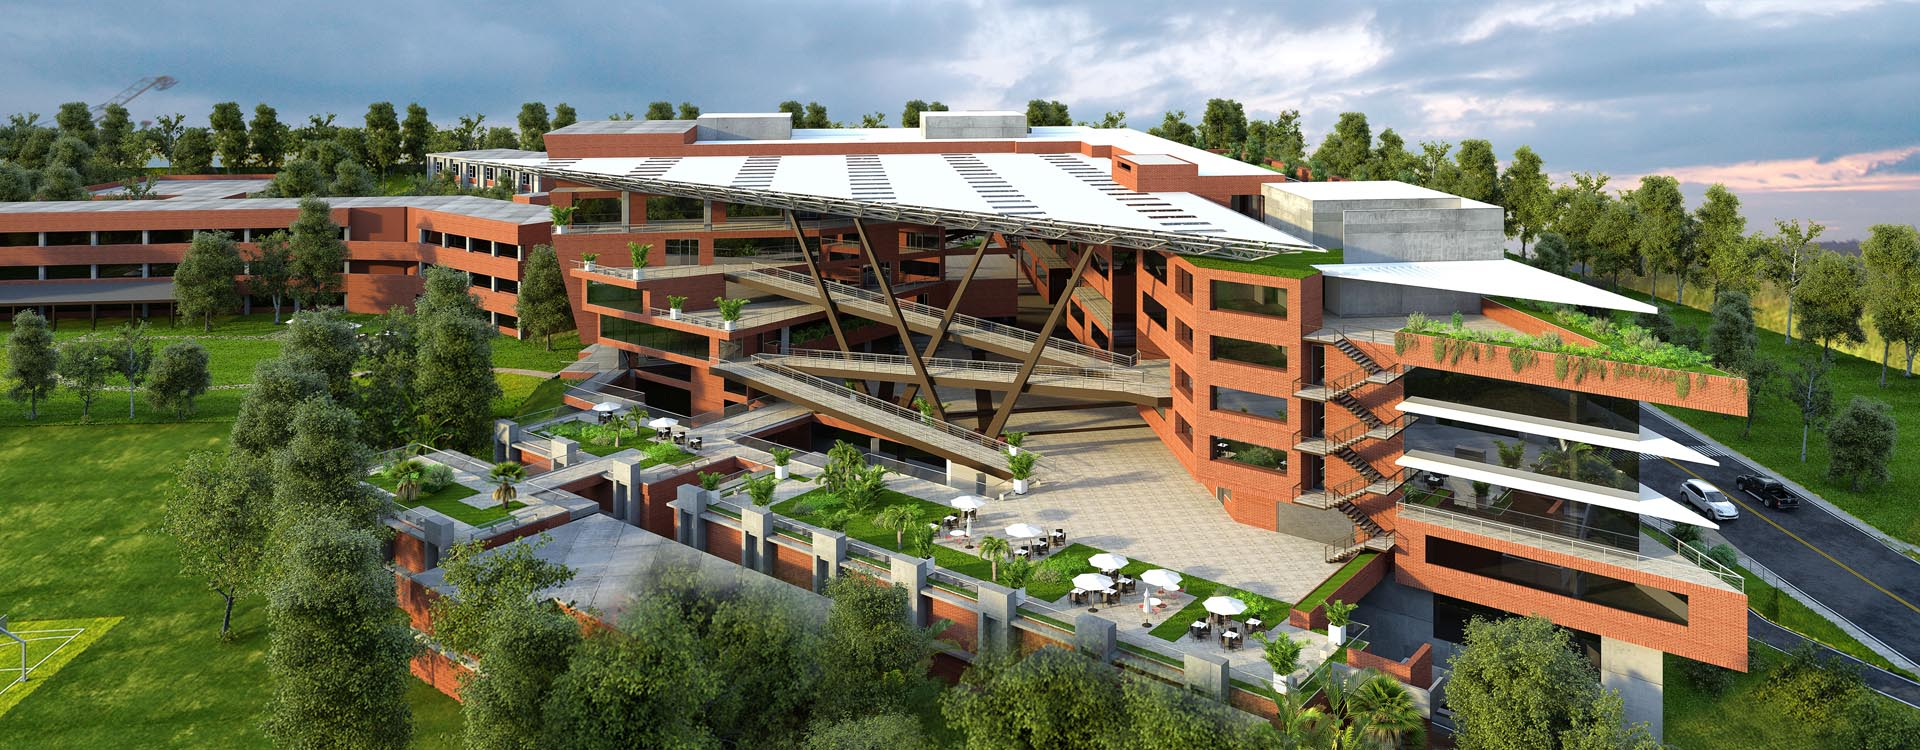
\includegraphics[height=13.25cm]{plantilla/portadacit.jpg}}
    	\makebox[\textwidth]{
    		\begin{overpic}[height=13.25cm]{\imagenportada}
     		\put(63,0){
\includegraphics[height=1.15in]{plantilla/fondologo_grande.png}}  
  			\put(64.5,2){
\includegraphics[height=0.55in]{plantilla/logoUVGblanco.eps}} 
        	\end{overpic}
    	}
    	%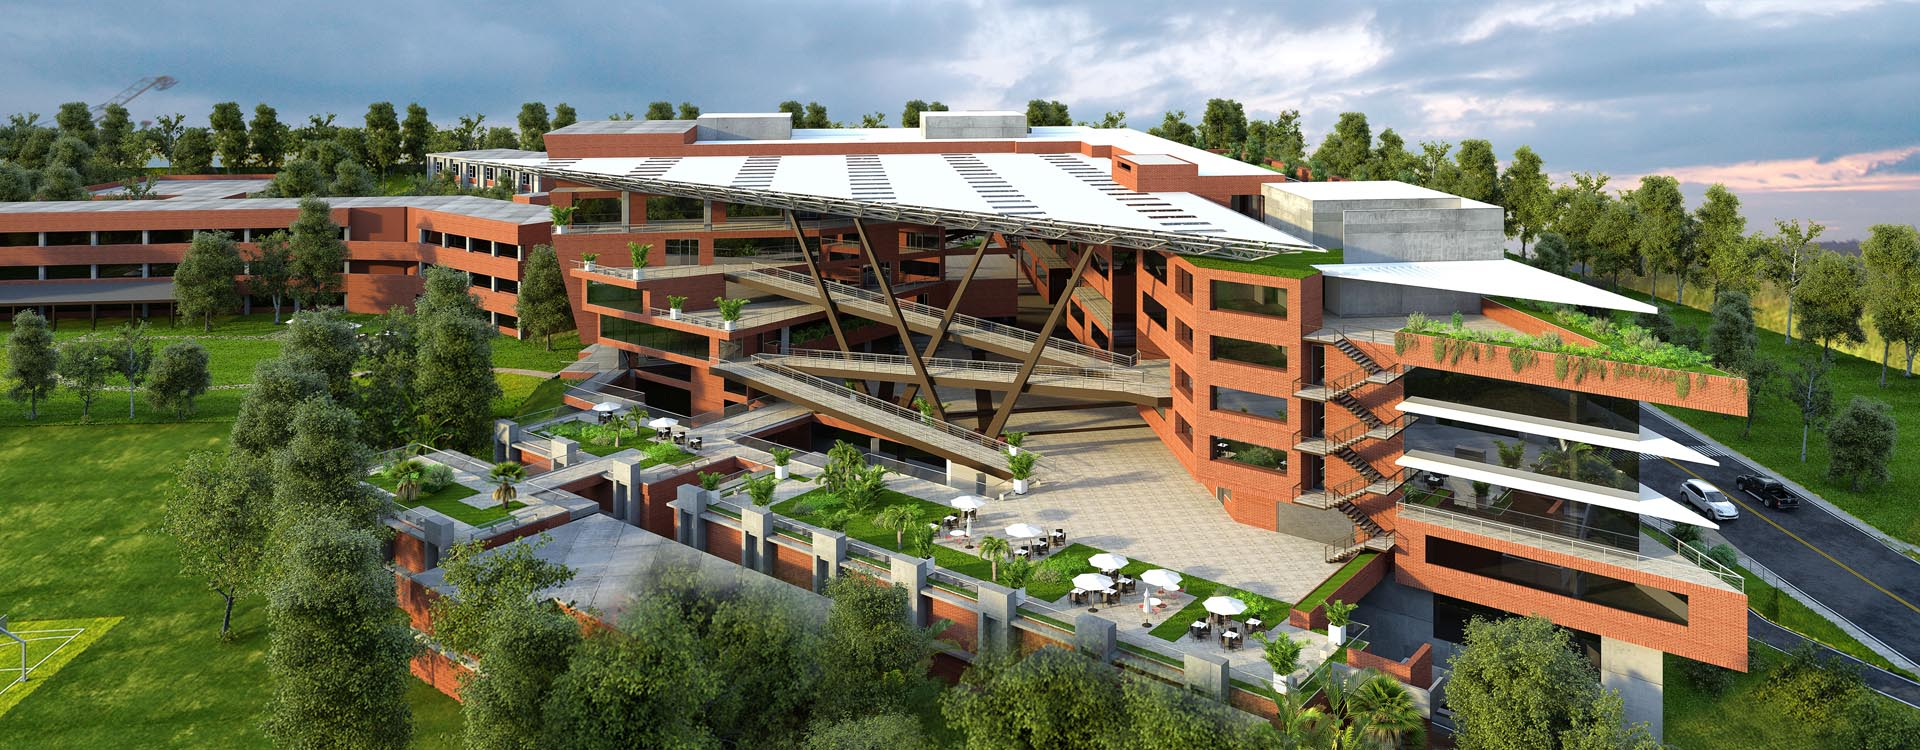
\includegraphics[height=13.25cm]{plantilla/portadacit.jpg}
	\end{figure}
	\restoregeometry
\fi

% ==============================================================================
% PRIMERAS PÁGINAS (Carátulas más hojas de guarda)
% ==============================================================================
\ifdefined\CAPcaratula
	\newpage
    \cleardoublepage\phantomsection
    % \pdfbookmark{Carátula}{toc}
	\pagecolor{white}
	\color{black}
	\setcounter{page}{1}
	\pagenumbering{roman}
	\thispagestyle{empty}
	\begin{center}
		\LARGE UNIVERSIDAD DEL VALLE DE GUATEMALA\\
		\LARGE Facultad de \uvgfacultad \\[0.75cm]
	\end{center}
	\begin{figure}[h]
		\begin{center}
		
\includegraphics[height=5.5 cm]{plantilla/escudoUVGnegro.eps}
		\vspace{0.5in}
		\end{center}
	\end{figure}
	\begin{center}
		\Large \textbf{\nohyphens{\titulotesis}} \\
		%\LARGE \textbf{\titulotesis} \\
		\vfill
		\Large \nohyphens{Trabajo de graduación presentado por \nombreestudiante \ para optar al grado académico de Licenciado en \uvgcarrera} \\
		\vfill
		\large Guatemala, \\
		\vspace{1em}
		\anoentrega
	\end{center}
    
    \ifdefined\printver	
	    \blankpage
	    \blankpage
	    
	    \newpage
	    \cleardoublepage\phantomsection
	    \pagecolor{white}
    	\color{black}
    	\setcounter{page}{1}
    	\pagenumbering{roman}
    	\thispagestyle{empty}
    	\begin{center}
    		\LARGE UNIVERSIDAD DEL VALLE DE GUATEMALA\\
    		\LARGE Facultad de \uvgfacultad \\[0.75cm]
    	\end{center}
    	\begin{figure}[h]
    		\begin{center}
    		
\includegraphics[height=5.5 cm]{plantilla/escudoUVGnegro.eps}
    		\vspace{0.5in}
    		\end{center}
    	\end{figure}
    	\begin{center}
    		\Large \textbf{\nohyphens{\titulotesis}} \\
    		%\LARGE \textbf{\titulotesis} \\
    		\vfill
    		\Large \nohyphens{Trabajo de graduación presentado por \nombreestudiante \ para optar al grado académico de Licenciado en \uvgcarrera} \\
    		\vfill
    		\large Guatemala, \\
    		\vspace{1em}
    		\anoentrega
    	\end{center}
    \fi
\fi

% ==============================================================================
% HOJA DE FIRMAS
% ==============================================================================
\ifdefined\CAPfirmas
	\newpage
	\cleardoublepage\phantomsection
	\thispagestyle{empty}
	\vspace*{0.5in}
	\large Vo.Bo.:\\[1cm]
	\begin{center}
		(f) \rule[1pt]{4 in}{1pt}\\
		\nombreasesor
	\end{center}
	\vspace{1in}

	Tribunal Examinador:\\[1cm]
	\begin{center}
		(f) \rule[1pt]{4 in}{1pt}\\
		\nombreasesor \\[1in]
		(f) \rule[1pt]{4 in}{1pt}\\
		\nombreprimerex \\[1in]
		(f) \rule[1pt]{4 in}{1pt}\\
		\nombresegundoex
	\end{center}
	\vspace{1in}

%	Fecha de aprobación: Guatemala, \rule[1pt]{0.5 in}{1pt} de \rule[1pt]{1 in}{1pt} de \anoaprobacion.
    Fecha de aprobación: Guatemala, \diaaprobacion de \mesaprobacion de \anoaprobacion.
	\normalsize
\fi

% Comentar para formato estilo libro en la numeración de páginas (NO 
% compatible con la guía UVG 2019)
\pagestyle{plain}
% ==============================================================================
% CONTENIDO DEL TRABAJO
% ==============================================================================
% PREFACIO
% ------------------------------------------------------------------------------
\ifdefined\CAPprefacio
	\newpage
	\cleardoublepage\phantomsection
    \chapter*{Prefacio}
    \ifdefined\parpordefecto
    	\defaultparformat{a-prefacio}
    \else
    	%INCLUIR, EN FORMA RESUMIDA, LOS PRINCIPALES RESULTADOS OBTENIDOS.

%No hacer referencias a figuras en el resumen.

%Aquí no vale la pena mencionar lo que NO se hizo.

En Guatemala no se cuenta con fácil acceso a nuevas tecnologías para el estudio a fondo de los casos de pacientes con epilepsia, que a la fecha se estiman que son alrededor de 325,000 pacientes; una enfermedad que repercute tanto en la salud del paciente como en su desenvolvimiento social. 
El presente trabajo tiene como objetivo, aplicar los algoritmos de aprendizaje automático desarrollados en fases anteriores a una mayor cantidad de señales bioeléctricas, y mejorar el proceso de detección de segmentos de interés en las señales, para el estudio de la epilepsia.

Para lograrlo se inició con la obtención de señales bioeléctricas con el equipo BIOPAC de la Universidad del Valle de Guatemala (UVG), de personas que no sufren de ataques epilépticos y por parte de HUMANA, señales bioeléctricas de pacientes con ataques de epilepsia.
Recolectar una mayor cantidad de datos que en años previos fue de gran necesidad, sirvió para una mejor clasificación al momento de entrenar el modelo de aprendizaje automático. Cabe destacar que a los datos obtenidos con el equipo de UVG, se les asignaba un nombre según la norma que se estableció en UVG. Posteriormente se extrajo características en el dominio del tiempo, frecuencia y wavelets de las señales anteriormente mencionadas. Los experimentos para la validación de modelos, en el caso de las señales de electromiografía (EMG) fueron intrasujeto, mientras que, en el caso de las señales de electroencefalografía (EEG) fueron intersujeto. 

Por ultimo, se actualizó la herramienta de software para el estudio de la epilepsia que se ha desarrollado en los últimos años. Esto incluía el mejoramiento del proceso de detección de segmentos de interés en las señales bioeléctricas, la optimización funciones para la extracción de características y el entrenamiento del modelo de aprendizaje automático y la generación automática de anotaciones relevantes. Cumplidas estas actividades se procedió con el análisis estadístico  para evaluar el rendimiento de los algoritmos e identificar posibles mejoras a los mismos.
    \fi
    \addcontentsline{toc}{chapter}{Prefacio}
\fi

% ÍNDICE GENERAL
% ------------------------------------------------------------------------------
\ifdefined\CAPindice
	\newpage
    \cleardoublepage\phantomsection
	\renewcommand{\contentsname}{Índice}
    %\phantomsection
    \pdfbookmark{\contentsname}{toc}
    %\pdfbookmark{Índice}{toc}
	\tableofcontents
\fi

% LISTADO DE FIGURAS
% ------------------------------------------------------------------------------
\ifdefined\CAPfiguras
	\newpage
    \cleardoublepage\phantomsection
	\renewcommand{\listfigurename}{Lista de figuras}
	\listoffigures
	\addcontentsline{toc}{chapter}{Lista de figuras}
\fi

% LISTADO DE CUADROS
% ------------------------------------------------------------------------------
\ifdefined\CAPcuadros
	\newpage
    \cleardoublepage\phantomsection
	\renewcommand{\listtablename}{Lista de cuadros}
	\listoftables
	\addcontentsline{toc}{chapter}{Lista de cuadros}
\fi

% RESUMEN
% ------------------------------------------------------------------------------
\ifdefined\CAPresumen
	\newpage
    \cleardoublepage\phantomsection
	\chapter*{Resumen}
	\ifdefined\parpordefecto
		\defaultparformat{b-resumen}
	\else
		%INCLUIR, EN FORMA RESUMIDA, LOS PRINCIPALES RESULTADOS OBTENIDOS.

%No hacer referencias a figuras en el resumen.

%Aquí no vale la pena mencionar lo que NO se hizo.

En Guatemala no se cuenta con fácil acceso a nuevas tecnologías para el estudio a fondo de los casos de pacientes con epilepsia, que a la fecha se estiman que son alrededor de 325,000 pacientes; una enfermedad que repercute tanto en la salud del paciente como en su desenvolvimiento social. 
El presente trabajo tiene como objetivo, aplicar los algoritmos de aprendizaje automático desarrollados en fases anteriores a una mayor cantidad de señales bioeléctricas, y mejorar el proceso de detección de segmentos de interés en las señales, para el estudio de la epilepsia.

Para lograrlo se inició con la obtención de señales bioeléctricas con el equipo BIOPAC de la Universidad del Valle de Guatemala (UVG), de personas que no sufren de ataques epilépticos y por parte de HUMANA, señales bioeléctricas de pacientes con ataques de epilepsia.
Recolectar una mayor cantidad de datos que en años previos fue de gran necesidad, sirvió para una mejor clasificación al momento de entrenar el modelo de aprendizaje automático. Cabe destacar que a los datos obtenidos con el equipo de UVG, se les asignaba un nombre según la norma que se estableció en UVG. Posteriormente se extrajo características en el dominio del tiempo, frecuencia y wavelets de las señales anteriormente mencionadas. Los experimentos para la validación de modelos, en el caso de las señales de electromiografía (EMG) fueron intrasujeto, mientras que, en el caso de las señales de electroencefalografía (EEG) fueron intersujeto. 

Por ultimo, se actualizó la herramienta de software para el estudio de la epilepsia que se ha desarrollado en los últimos años. Esto incluía el mejoramiento del proceso de detección de segmentos de interés en las señales bioeléctricas, la optimización funciones para la extracción de características y el entrenamiento del modelo de aprendizaje automático y la generación automática de anotaciones relevantes. Cumplidas estas actividades se procedió con el análisis estadístico  para evaluar el rendimiento de los algoritmos e identificar posibles mejoras a los mismos.
	\fi
	\addcontentsline{toc}{chapter}{Resumen}
\fi

% ABSTRACT
% ------------------------------------------------------------------------------
\ifdefined\CAPabstract
	\newpage
    \cleardoublepage\phantomsection
	\chapter*{Abstract}
	\ifdefined\parpordefecto
		\defaultparformat{c-abstract}
	\else
		In Guatemala there is no easy access to new technologies for the in-depth study of the cases of patients with epilepsy, which to date are estimated to be around 325,000 patients; a disease that affects both the patient's health and social development. 
The present work aims to apply the machine learning algorithms developed in previous phases to a larger number of bioelectrical signals, and to improve the process of detecting segments of interest in the signals, for the study of epilepsy.

To achieve this, we began by obtaining bioelectrical signals with the BIOPAC equipment of the Universidad del Valle de Guatemala (UVG), from people who do not suffer from epileptic seizures, and by HUMANA, bioelectrical signals from patients with epileptic seizures.
Collecting a larger amount of data, which in previous years was of great need, served for a better classification when training the machine learning model. It should be noted that the data obtained with the UVG equipment were assigned a name according to the standard that was established in UVG. Subsequently, time, frequency and wavelet domain features were extracted from the aforementioned signals. The experiments for model validation, in the case of electromyography (EMG) signals, were intrasubject, while in the case of electroencephalography (EEG) signals they were intersubject. 

Finally, the software tool for the study of epilepsy that has been developed in recent years was updated. This included improving the process of detecting segments of interest in the bioelectrical signals, optimizing functions for feature extraction and training of the machine learning model and automatic generation of relevant annotations. Once these activities were completed, statistical analysis was performed to evaluate the performance of the algorithms and identify possible improvements to them.
	\fi
	\addcontentsline{toc}{chapter}{Abstract}
\fi

% INTRODUCCIÓN
% ------------------------------------------------------------------------------
\ifdefined\CAPintroduccion
	\newpage
	\cleardoublepage
	\pagenumbering{arabic}
	\setcounter{page}{1}
	\chapter{Introducción}
	\ifdefined\parpordefecto
		\defaultparformat{d-introduccion}
	\else
		%PARAFRASEAR LOS OBJETIVOS GENERAL Y ESPECÍFICOS. (Es decir, cuál es el problema o situación que se desea resolver)

%PODRÍAN MENCIONAR LO QUE SE PRESENTARÁ EN ESTE DOCUMENTO, ES DECIR, CÓMO ESTÁ ORGANIZADO EL MISMO.

En este trabajo de investigación, se aborda el tema de la epilepsia, un trastorno neurológico común caracterizado por convulsiones recurrentes e incapacitantes, conocidas como crisis epilépticas, médicamente descrito como actividad ictal. Se ha observado un creciente interés en la aplicación del aprendizaje automático en aplicaciones clínicas y experimentales relacionadas con el diagnóstico de la epilepsia y otros trastornos neurológicos y psiquiátricos. Los métodos de aprendizaje automático son considerados como potenciales herramientas capaces de proporcionar un rendimiento fiable y óptimo en el diagnóstico clínico, la predicción y la medicina personalizada, mediante la aplicación de algoritmos matemáticos y enfoques computacionales.

Entre las aplicaciones que se han empleado con los algoritmos de aprendizaje automático en el contexto de la epilepsia, se encuentra el reconocimiento de patrones de interés en señales bioeléctricas. Este enfoque ha demostrado ser efectivo en la reducción del tiempo de diagnóstico, en contraposición al método tradicional de análisis y anotaciones manuales realizadas por los médicos, que tiende a ser una tarea que consume mucho tiempo, especialmente cuando se tratan registros de varias horas de duración.

El objetivo de este proyecto de investigación es aplicar los algoritmos de aprendizaje automático desarrollados en fases anteriores a una mayor cantidad de señales bioeléctricas, y mejorar el proceso de detección de segmentos de interés en las señales, para el estudio de la epilepsia.
Esto implica el análisis de diversas señales bioeléctricas y la evaluación de clasificadores. En trabajos previos, se emplearon características en el dominio del tiempo, frecuencia y se utilizaron transformadas Wavelet para el análisis. 
En este trabajo, se presenta una revisión de las bases teóricas utilizadas para abordar el problema, así como una descripción detallada de los experimentos realizados, la metodología empleada y los resultados obtenidos en el transcurso de esta investigación. Asimismo, se presentan las conclusiones y recomendaciones que surgen de este estudio, con miras a futuras investigaciones en esta área de estudio.


	\fi
\fi

% ANTECEDENTES
% ------------------------------------------------------------------------------
\ifdefined\CAPantecedentes
	\newpage
	\chapter{Antecedentes}
	\ifdefined\parpordefecto
    	\defaultparformat{e-antecedentes}
    \else
    	Las señales bioeléctricas y las señales de la epilepsia son temas de gran interés en la actualidad debido a su relevancia en la medicina y la neurociencia. La epilepsia es una enfermedad neurológica común que afecta a millones de personas en todo el mundo \cite{pichon2017patogenia}. La prevalencia de la enfermedad varía según el país y la región del mundo, siendo más común en niños y personas mayores, además, se estima que el 80\% de las personas con epilepsia vive en países de bajos y medianos ingresos, donde el acceso a los tratamientos puede ser limitado o inaccesible \cite{Epilepsia_OMS}.

En Guatemala, se encuentra el Centro de Epilepsia y Neurocirugía Funcional HUMANA, una organización formada por profesionales en neurociencias que trabaja con pacientes que padecen problemas neurológicos de difícil control, incluyendo la epilepsia. El centro posee el único laboratorio de vídeo electroencefalograma en Guatemala y lleva a cabo anotaciones de señales EEG manualmente, lo que implica una gran cantidad de horas de trabajo realizadas por profesionales especializados del hospital. El tiempo de operación para resaltar los segmentos de interés y finalmente dar el diagnóstico depende de la duración del registro y puede durar desde cuatro horas hasta algunos días \cite{humana_2021}. Según una entrevista realizada en 2020 al director de HUMANA, Dr. Juan Carlos Lara, las señales de donde se extraen los datos son obtenidas de personas sin y con padecimiento de epilepsias, lo que permite a los especialistas hacer las anotaciones competentes dentro de los registros \cite{camila_2022}.

En la Universidad del Valle de Guatemala (UVG) se ha estado desarrollando una herramienta de aprendizaje automático para la detección de crisis epilépticas en señales EEG. En el año 2020, María Jesús Angulo presentó un trabajo de graduación en el que se demostró que es posible detectar estas crisis mediante aprendizaje automático al caracterizar y dividir correctamente los segmentos de las señales \cite{María_ang_2020}. 

Por su parte, en el año 2021, David Alejandro Vela presentó una segunda iteración de la herramienta en su trabajo de graduación. En este caso, se realizaron ajustes a la interfaz anterior, empleando algoritmos de aprendizaje automático supervisado para clasificar la señal EEG en una de cuatro clases \cite{david_2022}. El clasificador con mejor desempeño en tiempo continuo obtuvo un promedio de exactitud del 96.7\%, utilizando máquina de vectores de soporte con características en tiempo continuo y kernel gaussiano. Además, se agregó una nueva sección a la herramienta que se encarga de la generación de anotaciones dentro de un apartado con varias opciones de personalización para la visualización. Aunque se trabajó principalmente con señales EEG en dominio del tiempo en ambas fases, se reconoce la oportunidad de analizar las señales en otros dominios y de analizar otro tipo de señales bioeléctricas. Una de las limitaciones del trabajo fue la predominancia del uso de técnicas de aprendizaje supervisado, lo que abre espacio para profundizar en el análisis de los datos con aprendizaje no supervisado. Los resultados de esta segunda fase se observan en la Figura~\ref{fig:mesh1} \cite{david_2022}. Además en la Figura~\ref{fig:app_ini} se puede ver la ventana inicial de la app y en la Figura~\ref{fig:app_chn_slct} se puede observar la forma en la que se clasifica un segmento de señal por color según su estado ictal.

\begin{figure}[t]
    \centering
    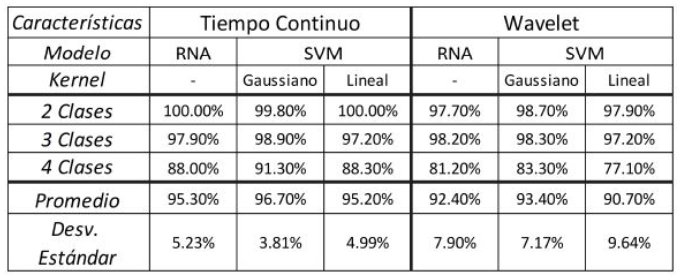
\includegraphics[width=0.5\textwidth]{figuras/David resultado.png}
    \caption{Resumen de los resultados de los clasificadores generados: red neuronal (RNN) y máquina de vectores de soporte (SVM) \cite{david_2022}.}
    \label{fig:mesh1}
\end{figure}

En el año 2022 Camila Lemus \cite{camila_2022} concluyó que las relaciones entre bandas de frecuencia son funcionales para la clasificación binaria, logrando un porcentaje de rendimiento superior al 99\% utilizando redes neuronales con dos o más características para las clases Ictal/Sano y superior a un 98.80\% para las clases Interictal/Preictal, dichos resultados se pueden observar en la Figura~\ref{fig:camila_tabla_res1}. Además, se encontró que es conveniente generar el vector de características combinando la razón 1 ($\theta/\alpha$) y la razón 2 ($\beta/\alpha$), ya que los clasificadores tienen un rendimiento igual o mayor a 98.90\% en un menor tiempo. Sin embargo, se observó que la extracción de características en dominio de la frecuencia no es muy eficiente, tardando en promedio aproximadamente 3 minutos por registro individual para procesar 409,700 muestras y 4.33 minutos para procesar 3 millones de muestras \cite{camila_2022}. El algoritmo utilizado para el análisis y el reconocimiento de patrones en señales de ECG fue \textit{K-means Clustering}. Los resultados mostraron que el algoritmo era capaz de identificar agrupaciones de señales de ECG asociadas a oscilaciones postictales de la frecuencia cardiaca. Esto sugiere que la agrupación de \textit{K-means Clustering} podría utilizarse para desarrollar un nuevo método de diagnóstico y seguimiento de la epilepsia.

\begin{figure}[t]
    \centering
    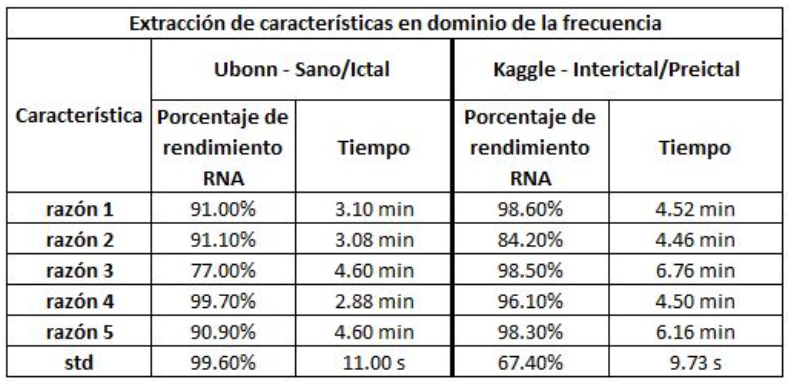
\includegraphics[width=0.5\textwidth]{figuras/3 rendimiento RNA Camila.png}
    \caption{Resumen del rendimiento de la RNN para dos clasificadores binarios utilizando características individuales en dominio de la frecuencia \cite{camila_2022}.}
    \label{fig:camila_tabla_res1}
\end{figure}

\begin{figure}[t]
    \centering
    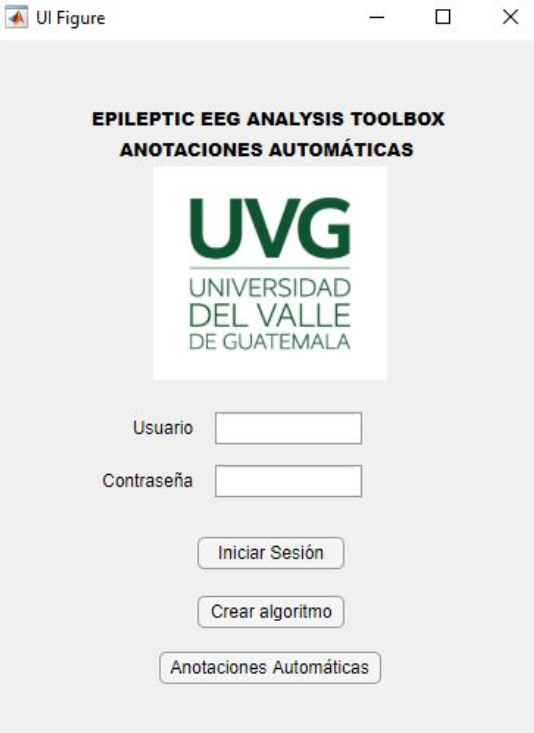
\includegraphics[width=0.5\textwidth]{figuras/4 incio app.png}
    \caption{Ventana de la aplicación para iniciar sesión \cite{david_2022}.}
    \label{fig:app_ini}
\end{figure}

\begin{figure}[ht]
    \centering
    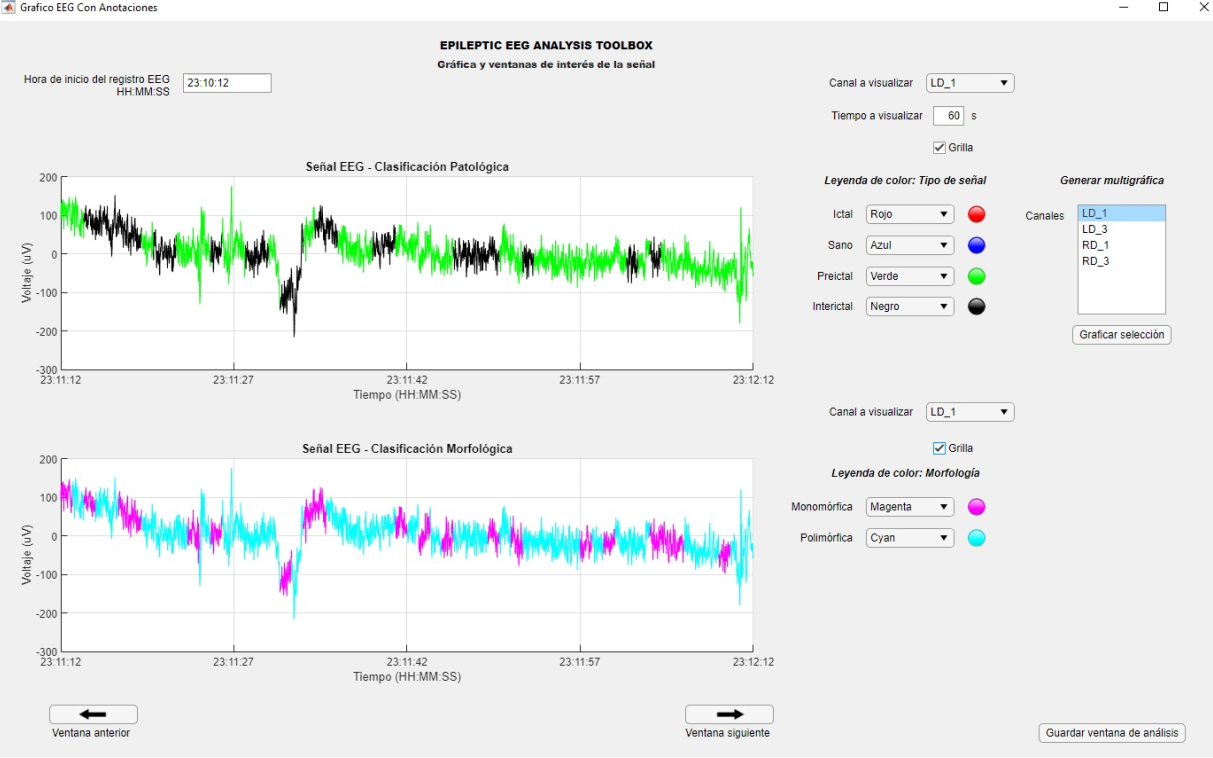
\includegraphics[width=0.5\textwidth]{figuras/5 app chn select.png}
    \caption{Ventana con la gráfica de una ventana del registro EEG del canal seleccionado \cite{david_2022}.}
    \label{fig:app_chn_slct}
\end{figure}

    \fi  
\fi

% JUSTIFICACIÓN
% ------------------------------------------------------------------------------
\ifdefined\CAPjustificacion
	\newpage
	\chapter{Justificación}
	\ifdefined\parpordefecto
		\defaultparformat{f-justificacion}
	\else
		En Guatemala, hay un acceso limitado a la atención médica, lo que se agrava en las zonas rurales donde la incidencia de la epilepsia es mayor. A pesar de la alta prevalencia de la epilepsia en el país, hay una escasa cantidad de investigaciones sobre esta afección, lo que hace necesario llenar este vacío en el conocimiento y obtener información importante sobre la epilepsia en esta población \cite{mendizabal1996prevalence}.

Para la continuación de esta línea de investigación se percibe la necesidad de ampliar la herramienta incorporando señales bioeléctricas de interés, como las de electromiograma (EMG). Asimismo, se ha recomendado continuar experimentando el rendimiento de los clasificadores con diferentes técnicas de aprendizaje automático no supervisado para señales EEG, ECG y otras señales bioeléctricas relacionadas con la epilepsia. Para la investigación que se realizo en el presente proyecto, se aplico la mejora del proceso de selección de características de las señales mediante asesoría médica y la validación constante con especialistas en el campo para mejorar la predicción de los clasificadores \cite{camila_2022}. 

El acceso a un mayor número de señales proporciona una muestra más representativa de la actividad bioeléctrica cerebral y muscular de los pacientes epilépticos. Esto permite una comprensión más completa y precisa de los patrones y características de las señales relacionadas con la epilepsia, lo que conduce a una mejor comprensión de la enfermedad y sus diversas manifestaciones \cite{rouhiainen2018inteligencia}.

La aplicación de algoritmos de agrupación a un mayor número de señales de EEG y EMG puede ayudar a identificar subgrupos o patrones ocultos dentro de la población de pacientes con epilepsia \cite{felix2002data}. Estos subgrupos pueden tener relevancia clínica, como diferentes tipos de epilepsia, respuestas variadas al tratamiento o diferencias en la gravedad de los síntomas. Al identificar estos subgrupos, los profesionales sanitarios pueden adaptar el tratamiento y los cuidados de forma más precisa a cada paciente, personalizando así su enfoque médico.

En este trabajo se busca, además de, aplicar algoritmos de aprendizaje automático a una mayor cantidad de señales bioeléctricas también, implementar un algoritmo que pueda indicar en qué tiempo de la grabación se encuentran señales de interés para su estudio, con el fin de aprovechar de forma óptima el tiempo disponible. Actualmente, las grabaciones pueden durar hasta 24 horas y los médicos deben analizar toda la grabación para detectar la actividad bioeléctrica de interés. Este proceso resulta muy ineficiente.


	\fi
\fi

% OBJETIVOS
% ------------------------------------------------------------------------------
\ifdefined\CAPobjetivos
	\newpage
	\chapter{Objetivos}
	\ifdefined\parpordefecto
		\defaultparformat{g-objetivos}
	\else
		\subsection*{Objetivo General}
Aplicar los algoritmos de aprendizaje automático desarrollados en fases anteriores a una mayor cantidad de señales bioeléctricas, y mejorar el proceso de detección de segmentos de interés en las señales, para el estudio de la epilepsia.

\subsection*{Objetivos Específicos}
\begin{itemize}
\item Obtener una buena cantidad de señales bioeléctricas capturadas con el equipo de la UVG, y de pacientes con epilepsia de HUMANA.
\item Aplicar algoritmos de aprendizaje automático desarrollados en fases anteriores, para la extracción de características de las señales bioeléctricas del tipo EEG y EMG.
\item Mejorar el proceso de detección de segmentos de interés en las señales y la generación automática de anotaciones relevantes, según los parámetros de HUMANA.
\item Realizar análisis estadísticos para evaluar el rendimiento de los algoritmos e identificar posibles mejoras a los mismos.
\item Actualizar la herramienta de software para el estudio de la epilepsia desarrollada en fases anteriores, incorporando las mejoras a los algoritmos de clasificación y detección de segmentos de interés de las señales bioeléctricas.
\end{itemize}

%Enumeración 
%\begin{enumerate}
%\item Nulla ut ex ut mauris pretium elementum.
%\item Suspendisse malesuada lectus nec nisi iaculis, in luctus turpis laoreet.
%\item In efficitur nisl vitae justo interdum, vitae condimentum lectus maximus.
%\item Morbi quis libero sit amet velit commodo tristique eu sed nisl.
%\end{enumerate}
	\fi
\fi

% ALCANCE
% ------------------------------------------------------------------------------
\ifdefined\CAPalcance
	\newpage
	\chapter{Alcance}
	\ifdefined\parpordefecto
    	\defaultparformat{h-alcance}
    \else
    	%Podemos usar \Gls{latex} para escribir de forma ordenada una \gls{formula} matemática. 

%¿HASTA DÓNDE SE LLEGÓ CON ESTE PROYECTO? ¿QUÉ RESOLVIÓ, QUÉ QUEDÓ PARA TRABAJOS FUTUROS?  Basarse en los objetivos cumplidos.

%NO ENTRAR EN DETALLES TÉCNICOS O VALORES ESPECÍFICOS EN ESTA SECCIÓN. LA EXPLICACIÓN DE LOS ALCANCES DEBE SER MÁS GENERAL.

%Revisar los tiempos verbales. No usar tiempo futuro para describir cosas que ya hicieron.

%No incluir recomendaciones en este capítulo. Dejarlas para el capítulo de recomendaciones.

Los resultados derivados de este estudio se aplicarán principalmente en el contexto de Guatemala, aunque las metodologías desarrolladas pueden ser de utilidad en otros entornos médicos similares. Para este trabajo de graduación se recopilaron señales electroencefalográficas y electromiográficas capturadas con el equipo de la Universidad del Valle de Guatemala (UVG). Se obtuvieron señales señales bioeléctricas de pacientes con epilepsia atendidos en el Instituto HUMANA, ubicado en Guatemala. 

Los algoritmos de aprendizaje automático se aplicaron específicamente para la extracción de características de las señales bioeléctricas, la detección de patrones de interés y la generación de anotaciones relevantes. Estos algoritmos se basaron en técnicas de aprendizaje supervisado y no supervisado. No se abordó la investigación de nuevos algoritmos de aprendizaje automático en este trabajo, sino la adaptación y optimización de técnicas existentes.

La actualización de la herramienta de software propuesta se enfocó en la mejora de los algoritmos empleados, así como aplicar buenas practicas de programación, obteniendo una optimización en cuanto al costo computacional. Se incluyó la exportación de datos de los segmentos de interés a analizar. 
La implementación de tratamientos médicos y decisiones clínicas a partir de los resultados obtenidos con la herramienta, estuvo fuera del alcance de este trabajo.

 %Esta herramienta permitió la detección y anotación de eventos epilépticos, así como la generación de informes que fueron revisados por especialistas médicos para su validación.
    \fi 
\fi

% MARCO TEÓRICO
% ------------------------------------------------------------------------------
\ifdefined\CAPmarcoteorico
	\newpage
	\chapter{Marco teórico}
	\ifdefined\parpordefecto
		\defaultparformat{i-marco_teorico}
	\else
		\section{Epilepsia}
La epilepsia es uno de los primeros trastornos documentados en la historia de la neurología. Su aparición se remonta a más de 3.000 años atrás, siendo mencionada por primera vez en la antigua Babilonia. No obstante, fue en el año 400 a.C. cuando Hipócrates señaló que la epilepsia era un trastorno cerebral. La palabra ``epilepsia'' proviene del griego y significa ``ataque''. A lo largo de la historia, el peculiar comportamiento provocado por ciertos tipos de crisis convulsivas ha dado lugar a numerosas supersticiones y prejuicios \cite{wyllie2006treatment}.

Una crisis epiléptica consiste en una alteración brusca y transitoria ocasionada por una actividad anormal de las neuronas, manifestándose a través de sensaciones, emociones y comportamientos extraños, espasmos musculares y pérdida de conciencia. La epilepsia implica una predisposición a experimentar crisis epilépticas recurrentes, siendo diagnosticada cuando una persona ha experimentado dos o más de estas crisis. Las crisis epilépticas se dividen en dos tipos principales: crisis generalizadas y crisis parciales o focales. En las crisis generalizadas, la descarga epiléptica afecta simultáneamente a toda la superficie del cerebro, mientras que en las crisis parciales o focales, la descarga epiléptica se origina en una parte específica del cerebro \cite{garcia2011feen}.

\subsection{Tipos de epilepsia}
Existen varios tipos de epilepsia, que se clasifican en función del tipo de crisis que experimenta una persona. Algunos tipos comunes de epilepsia son:
\begin{itemize}
    \item Epilepsia focal: Las crisis focales, también llamadas crisis parciales, se originan en una parte específica del cerebro. Estas crisis pueden hacer que la persona experimente sensaciones o movimientos en un lado del cuerpo.
    \item Epilepsia generalizada: Las crisis generalizadas afectan a ambos lados del cerebro. Estas crisis pueden hacer que la persona pierda el conocimiento, caiga al suelo y experimente espasmos musculares o convulsiones.
    \item Epilepsia de ausencia: Las crisis de ausencia, también llamadas crisis de pequeño mal, hacen que la persona se quede con la mirada perdida y pierda temporalmente la conciencia de lo que le rodea.
    \item Epilepsia tónico-clónica: Las crisis tónico-clónicas, también llamadas crisis de gran mal, son el tipo de crisis más conocido. Implican pérdida de conocimiento, caída al suelo y movimientos espasmódicos repetitivos del cuerpo.
    \item Epilepsia mioclónica juvenil: Este tipo de epilepsia suele comenzar en la adolescencia. Se caracteriza por breves sacudidas o espasmos musculares, especialmente por la mañana después de despertarse. 
\end{itemize}

\begin{figure}[t]
    \centering
    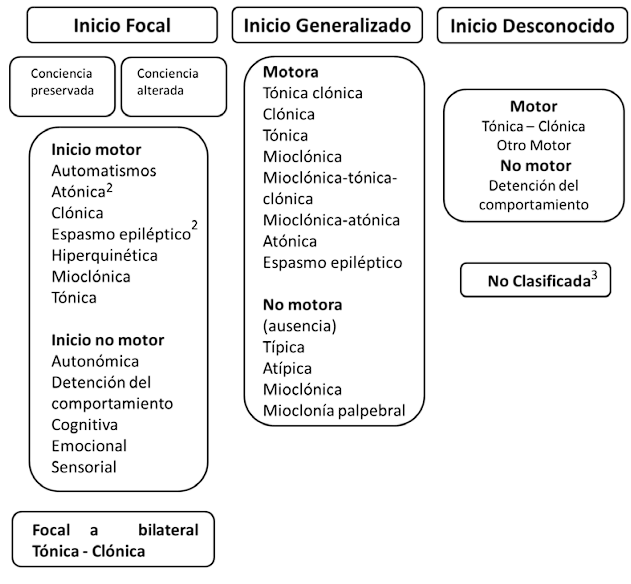
\includegraphics[width=0.5\textwidth]{figuras/6 Ictal_class.png}
    \caption{Clasificación Operacional Extendida de los tipos de crisis \cite{Clasificacion_ictal_imag}.}
    \label{fig:clasificacion_ictal_ref_imag}
\end{figure}

La Liga Internacional contra la Epilepsia (ILAE) ha introducido una categorización operativa actualizada de los tipos de crisis, mostradas en la Figura~\ref{fig:clasificacion_ictal_ref_imag}. La clasificación general incluye las crisis generalizadas, las crisis focales, también denominadas crisis de inicio parcial, y las crisis de origen desconocido. Estos tipos de crisis se clasifican a su vez en subcategorías basadas en síntomas motores y no motores. Además, en el caso de las crisis focales, existe otra distinción entre las que cursan con consciencia normal y las que presentan un nivel de consciencia alterado \cite{Clasificacion_ictal_imag}. 

\section{Señales bioeléctricas}
Las señales bioeléctricas son señales eléctricas producidas en los seres vivos que pueden medirse y controlarse continuamente. Estas señales suelen ser generadas por sistemas especializados de tejidos, órganos o células, como el sistema nervioso. Las señales bioeléctricas tienen características únicas que las hacen útiles en una amplia gama de aplicaciones, como la cardiología, la neurología y la ingeniería biomédica \cite{señales_unam}.

\section{Señales electroencefalográficas}
La electroencefalografía (EEG) es una prueba de diagnóstico neurofisiológico que consiste en la medición de la actividad eléctrica cerebral en estado de reposo, vigilia o sueño, y durante diversas activaciones. En general, la electroencefalografía se utiliza para el análisis de la actividad eléctrica cerebral en humanos con el fin de obtener información para una inspección exhaustiva de la funcionalidad cerebral, ayudando a la detección y prevención de enfermedades y trastornos. Estas ondas cerebrales se conocen como señales electroencefalográficas (señales EEG), que proporcionan información indirecta relacionada con las funciones cerebrales, incluidas, entre otras, las tareas mentales, las acciones motoras y las expresiones faciales \cite{manipula_arm_eeg}.

\subsection{Ritmos y formas de onda del EEG}
A continuación se resumen brevemente las características de los ritmos y formas de onda más frecuentes, que también se puede observar en la Figura~\ref{fig:eeg_ritmo_cerebral}. 
Las señales EEG registradas tienen, en amplitudes que oscilan entre unos pocos micro-voltios y aproximadamente 100 uV y un contenido frecuencial que oscila entre 0.5 y 30-40 Hz. Los ritmos electroencefálicos, también denominados ritmos de fondo, se clasifican convencionalmente en cinco bandas de frecuencia diferentes. La interpretación de estas bandas en términos de ``normal'' o ``anormal'' es relativa y depende de la edad y el estado mental del sujeto. Por ejemplo, el EEG de un recién nacido es drásticamente diferente del de un adulto y tiene, en general, un contenido de frecuencias considerablemente más alto.
\begin{itemize}
    \item Ritmo delta, <4 Hz. El ritmo delta suele aparecer durante el sueño durante profundo y tiene una gran amplitud. El adulto despierto y normal, pero es indicativo, por ejemplo, de daño cerebral o enfermedad cerebral (encefalopatía).
    \item Ritmo theta, 4-7 Hz. El ritmo theta se produce durante la somnolencia y en ciertas fases del sueño.
    \item Ritmo alfa, 8-13 Hz. Este ritmo es más prominente en sujetos normales que están relajados y despiertos con los ojos cerrados; la actividad se suprime cuando los ojos están abiertos. Cuando los ojos están abiertos. La amplitud del ritmo alfa es mayor en las regiones occipitales.
    \item Ritmo beta, 14-30 Hz. Es un ritmo rápido de baja amplitud, asociado a la activación de la corteza cerebral. Asociado a un córtex activado y que puede observarse, por ejemplo, durante ciertas fases del sueño. El ritmo beta se observa principalmente en las áreas frontal y central del cuero cabelludo.
    \item Ritmo gamma, >30 Hz. El ritmo gamma está relacionado con un estado de procesamiento activo de la información en el córtex. Utilizando un electrodo ubicado sobre el área sensoriomotora y conectado a una técnica de registro de alta sensibilidad, se puede observar el ritmo gamma.
\end{itemize}

\begin{figure}[t]
    \centering
    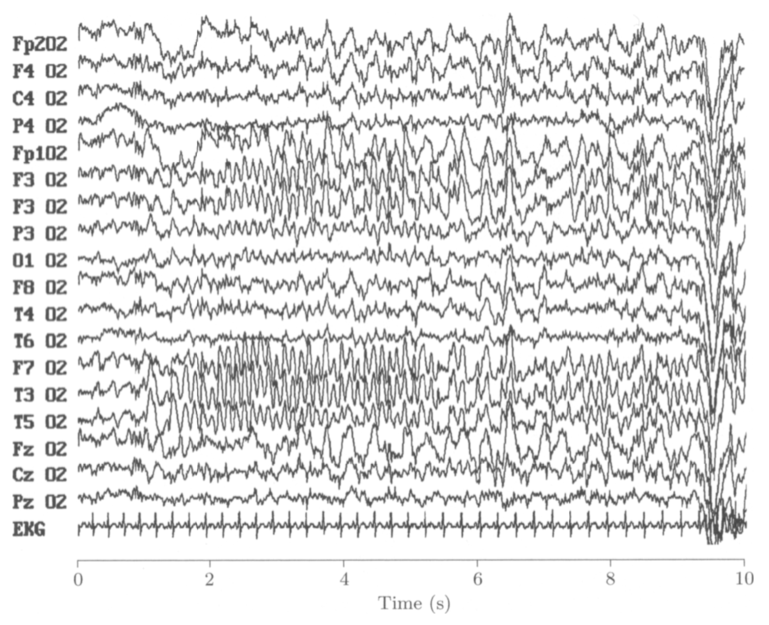
\includegraphics[width=0.5\textwidth]{figuras/7_ej_ictal_eeg.png}
    \caption{EEG multicanal que muestra el inicio de un ataque epiléptico después del primer segundo. El inicio se caracteriza por un aumento en la amplitud y un cambio en el contenido espectral. La convulsión es particularmente pronunciada en ciertos canales. Tenga en cuenta que el ECG se muestra en la parte inferior \cite{Libro_SP_cocoro_neuro_app}.}
    \label{fig:ej_ictal_multicanal_book}
\end{figure}
La mayoría de estos ritmos pueden durar varios minutos, mientras que otros sólo unos segundos. Es importante darse cuenta de que un ritmo no está presente en todo momento, una señal irregular de aspecto ``arrítmico'' \cite{Libro_SP_cocoro_neuro_app}.

\subsection{Picos y ondas agudas}
Los picos y las ondas agudas, también conocidas como SSW, son patrones distintivos en las formas de onda de EEG que tienen un patrón temporal esporádico e impredecible que indica un comportamiento neural anormal. Estos patrones se observan a menudo en pacientes que padecen epilepsia y se denominan interictales, ya que ocurren entre ataques epilépticos.

\begin{figure}[t]
    \centering
    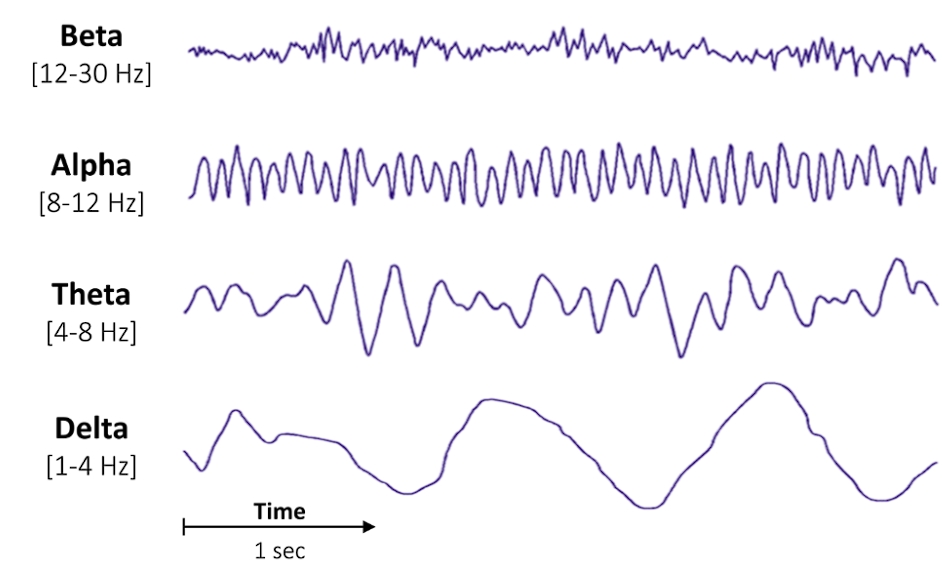
\includegraphics[width=0.5\textwidth]{figuras/8 Ritmo_cerebral_eeg.png}
    \caption{Ejemplo de ritmos cerebrales presentes en un EEG \cite{Vallat_2018}.}
    \label{fig:eeg_ritmo_cerebral}
\end{figure}

La definición de SSW es un poco ambigua, pero generalmente se caracteriza por un fuerte ascenso inicial que lo diferencia de un pico, que dura entre 20 y 70 ms. Por otro lado, SSW puede durar de 70 a 200 ms y exhibir formas de onda bifásicas y trifásicas. La morfología de SSW difiere según la ubicación del electrodo en el cuero cabelludo.

SSW puede ocurrir como eventos individuales o en series llamadas complejos de pico y onda, que consisten en un pico seguido de una onda lenta. La tasa de repetición de estos complejos puede oscilar entre menos de 3 a 6 Hz, y la tasa a menudo se asocia con diferentes interpretaciones clínicas.

Algunos artefactos EEG normales pueden parecerse a SSW, como la actividad cardíaca que puede hacerse pasar por un pico, particularmente las ondas del complejo QRS \cite{Libro_SP_cocoro_neuro_app}.

\subsection{Características de una señal EEG}
Hay una serie de características que se pueden extraer de las señales de EEG para su procesamiento. Estas funciones se pueden dividir en dos categorías principales: funciones en el dominio del tiempo y funciones en el dominio de la frecuencia.

\subsection{EEG ictal}
En el caso de una convulsión, el EEG se denomina EEG ictal y se caracteriza por un patrón inusual con un aumento repentino de la amplitud, como se muestra en la Figura~\ref{fig:ej_ictal_multicanal_book}. Además, el comienzo de una convulsión se acompaña de un cambio repentino en la amplitud. contenido de frecuencia que con frecuencia progresa a un patrón de picos y ondas. Debido a la variabilidad sustancial en el EEG ictal entre convulsiones, puede ser un desafío identificar el patrón de manera consistente, ya sea por medios manuales o automáticos \cite{Libro_SP_cocoro_neuro_app}.

\subsection{Procesamiento de señales EEG}
Las diferentes formas de onda de la señal EEG llevan información clínicamente valiosa. Una forma de onda puede representar un evento aislado, o varias formas de onda pueden constituir un patrón de señal compuesto. En ambos casos, es fundamental desarrollar métodos para detectar y cuantificar objetivamente las características de la señal para facilitar la interpretación visual. La extracción de características de señales relevantes es particularmente crucial cuando el objetivo es diseñar un sistema de clasificación de EEG. La cancelación de ruido y artefactos es otro tema importante en el procesamiento de señales de EEG y un requisito previo para el análisis de señales posterior confiable \cite{Libro_SP_cocoro_neuro_app}.

\section{Señales electromiográficas}
La electromiografía (EMG) es una herramienta de diagnóstico utilizada para analizar y registrar la actividad eléctrica producida por los músculos esqueléticos. La EMG se emplea en diversos campos de la medicina, como la neurología, la medicina deportiva, la rehabilitación y el diagnóstico. Los investigadores también utilizan la EMG para estudiar los patrones de activación muscular durante el movimiento, así como los patrones de fatiga y recuperación muscular. La EMG registra la actividad eléctrica llevada a cabo por las neuronas motoras durante las contracciones musculares y también mide la fuerza de las contracciones \cite{emg_def}. 

\section{Señales electrocardiográficas}
Un electrocardiograma (ECG) es una prueba médica común que registra la actividad eléctrica del corazón. Se utiliza para evaluar la salud y el funcionamiento del corazón, y puede ayudar a diagnosticar problemas cardíacos o monitorizar afecciones existentes. Durante un ECG, se colocan electrodos en el pecho, las extremidades y a veces en otros lugares del cuerpo, para medir y registrar la actividad eléctrica del corazón \cite{ecg_def}.

La prueba es indolora y no invasiva, lo que significa que no se introduce nada en el cuerpo. Los resultados del ECG proporcionan información sobre la frecuencia cardíaca, el ritmo cardíaco, la regularidad de los latidos y la presencia de cualquier anormalidad en la conducción eléctrica del corazón \cite{zavala2017descripcion}.


\section{Características en el dominio del tiempo}
Las características en el dominio del tiempo se basan en el análisis de la amplitud de la señal y sus cambios a lo largo del tiempo \cite{carac_time}. Algunas características comunes en el dominio del tiempo incluyen:
\begin{itemize}
    \item Media: 
    El valor promedio de la señal durante un intervalo de tiempo específico.
    \item Mediana: 
    El valor medio de la señal durante un intervalo de tiempo específico.
    \item Varianza: 
    La desviación cuadrada promedio de la señal de su valor medio.
    \item Desviación estándar: 
    La raíz cuadrada de la varianza.
    \item Asimetría: 
    Una medida de la asimetría de la distribución de la señal.
    \item Curtosis: 
    Una medida del pico de la distribución de la señal.
\end{itemize}

\section{Características en el dominio de frecuencia}
Las características en el dominio de la frecuencia se basan en el análisis del espectro de potencia de la señal. El espectro de potencia es un gráfico de la potencia de la señal en función de la frecuencia \cite{carac_freq}. Algunas características comunes en el dominio de la frecuencia incluyen:
\begin{itemize}
    \item Potencia: 
    La potencia total de la señal en una banda de frecuencia especificada.
    \item Energía: 
    La energía total de la señal en una banda de frecuencia específica.
    \item Densidad espectral: 
    La potencia de la señal por unidad de frecuencia en una banda de frecuencia especificada.
    \item Frecuencia centroide: 
    La frecuencia en la que el espectro de potencia de la señal es más alto.
    \item Propagación: 
    Una medida del ancho del espectro de potencia de la señal.
\end{itemize}

La elección de características para extraer de las señales de EEG depende de la aplicación. Por ejemplo, las funciones en el dominio del tiempo se usan a menudo para estudiar los cambios en la actividad cerebral a lo largo del tiempo, mientras que las funciones en el dominio de la frecuencia se usan a menudo para estudiar las diferentes bandas de frecuencia de la actividad cerebral \cite{al2014methods}.


\section{Propiedades de las señales deterministas y estocásticas}
Las señales deterministas son aquellas que pueden describirse mediante un conjunto de ecuaciones que definen su comportamiento en el tiempo. Las señales estocásticas, por otro lado, son aquellas que se caracterizan por fluctuaciones aleatorias.
Surge una pregunta fundamental con respecto a si el EEG debe verse como una señal determinista o estocástica. Los intentos de responder a esta pregunta pueden proporcionar información sobre los mecanismos de generación de EEG, pero también tienen implicaciones para los métodos de análisis de señales apropiados considerados. Generalmente, las características exactas de la señal EEG en términos de amplitud, duración o morfología de las ondas individuales no se pueden predecir, por lo que es bastante natural percibir la señal EEG como la realización de un proceso estocástico. Esta perspectiva cobra mayor fuerza al observar que no es posible adquirir una señal EEG ``pura'' que refleje únicamente la actividad cerebral. De hecho, siempre hay un ruido aleatorio corruptor introducido, por ejemplo, por el ruido interno en el equipo de amplificación o en el proceso de digitalización, lo que, incluso si el EEG ``puro'' tuviera propiedades deterministas, en última instancia hace que sea razonable considerar el EEG como un proceso estocástico \cite{Libro_SP_cocoro_neuro_app}.

Hay una serie de propiedades que se pueden utilizar para distinguir entre señales deterministas y estocásticas en los datos de EEG. Una propiedad es el espectro de potencia de la señal. El espectro de potencia de una señal es un gráfico de la potencia de la señal en función de la frecuencia. Las señales deterministas suelen tener un espectro de potencia que se caracteriza por picos pronunciados en frecuencias específicas. Las señales estocásticas, por otro lado, suelen tener un espectro de potencia que se distribuye de manera más uniforme entre las frecuencias \cite{Libro_SP_cocoro_neuro_app}.

Otra propiedad que se puede utilizar para distinguir entre señales deterministas y estocásticas es la función de autocorrelación de la señal. La función de autocorrelación de una señal es un gráfico de la correlación entre la señal y ella misma en diferentes lapsos de tiempo. Las señales deterministas suelen tener una función de autocorrelación que decae rápidamente con el tiempo. Las señales estocásticas, por otro lado, suelen tener una función de autocorrelación que decae más lentamente con el tiempo \cite{Libro_SP_cocoro_neuro_app}.

Finalmente, las señales deterministas y estocásticas también se pueden distinguir por su previsibilidad. Las señales deterministas son predecibles en el sentido de que su comportamiento futuro puede predecirse a partir de su comportamiento pasado. Las señales estocásticas, por otro lado, no son predecibles en el sentido de que su comportamiento futuro no puede predecirse a partir de su comportamiento pasado \cite{Libro_SP_cocoro_neuro_app}.

\section{Aprendizaje automático}
El aprendizaje automático (\textit{Machine Learning}) es un tipo de inteligencia artificial (IA) que permite a las aplicaciones de software ser más precisas en la predicción de resultados sin estar explícitamente programadas para ello. Los algoritmos de aprendizaje automático utilizan datos históricos como entrada para predecir nuevos valores de salida \cite{G-Cloud_2023}. Existen tres tipos principales de aprendizaje automático:
\begin{itemize}
    \item Aprendizaje supervisado
    \item Aprendizaje no supervisado
    \item Aprendizaje por refuerzo
\end{itemize}


\subsection{Aprendizaje supervisado}
El aprendizaje supervisado es un tipo de aprendizaje automático en el que el modelo se entrena en un conjunto de datos etiquetados. Esto significa que los datos se han etiquetado con la salida correcta. El modelo aprende a predecir la salida de nuevos datos en función de los datos etiquetados en los que se ha entrenado.

El aprendizaje supervisado se utiliza para una variedad de tareas, incluidas la clasificación, la regresión y la previsión. Las tareas de clasificación implican predecir la categoría de un punto de datos, como si un correo electrónico es spam o no. Las tareas de regresión implican predecir un valor numérico, como el precio de una casa. Las tareas de previsión implican predecir valores futuros, como el número de ventas en un mes determinado \cite{G-Cloud_2023}.

Hay muchos modelos diferentes de aprendizaje supervisado, cada uno con sus propias fortalezas y debilidades. Algunos de los modelos de aprendizaje supervisado más comunes incluyen:

\begin{itemize}
    \item Regresión lineal
    \item Regresión logística
    \item Árboles de decisión
    \item Bosques aleatorios
    \item Máquinas de vectores de soporte 
\end{itemize}

La elección de qué modelo de aprendizaje supervisado usar depende de la tarea específica en cuestión. Por ejemplo, la regresión lineal es una buena opción para tareas de regresión simples, mientras que los árboles de decisión son una buena opción para tareas más complejas.

El aprendizaje supervisado es una herramienta poderosa que se puede utilizar para resolver una variedad de problemas. Sin embargo, es importante tener en cuenta que los modelos de aprendizaje supervisado son tan buenos como los datos con los que se entrenan. Si los datos no son precisos o representativos del mundo real, el modelo no podrá hacer predicciones precisas \cite{nguyen2015aprendizaje}.

Estas son algunas de las características del aprendizaje supervisado:

\begin{itemize}
    \item Requiere datos etiquetados.
    \item Se utiliza para entrenar modelos para predecir valores de salida.
    \item Se puede utilizar para tareas de clasificación, regresión y previsión.
    \item Hay muchos modelos diferentes de aprendizaje supervisado disponibles.
    \item La elección del modelo depende de la tarea específica a realizar.
\end{itemize}

\subsection{Aprendizaje no supervisado}
El aprendizaje no supervisado es un tipo de aprendizaje automático en el que el modelo se entrena en un conjunto de datos no etiquetados. Esto significa que los datos no tienen etiquetas asociadas. El modelo aprende a encontrar patrones en los datos y a agrupar puntos de datos similares.

El aprendizaje no supervisado se utiliza para una variedad de tareas, incluida la agrupación, la reducción de la dimensionalidad y la detección de anomalías. Las tareas de agrupamiento implican agrupar puntos de datos en función de sus similitudes. Las tareas de reducción de dimensionalidad implican reducir la cantidad de características en un conjunto de datos mientras se conserva la mayor cantidad de información posible. Las tareas de detección de anomalías implican identificar puntos de datos que son significativamente diferentes del resto de los datos \cite{G-Cloud_2023}.

Hay muchos modelos diferentes de aprendizaje no supervisado, cada uno con sus propias fortalezas y debilidades. Algunos de los modelos de aprendizaje no supervisado más comunes incluyen:

\begin{itemize}
    \item Agrupamiento de K-medias
    \item Agrupación jerárquica
    \item Análisis de componentes principales (PCA)
    \item Descomposición en valores singulares (SVD)
    \item Modelos de mezcla gaussiana (GMM)
\end{itemize}

La elección de qué modelo de aprendizaje no supervisado usar depende de la tarea específica en cuestión. Por ejemplo, el agrupamiento de k-medias es una buena opción para tareas de agrupamiento simples, mientras que el agrupamiento jerárquico es una buena opción para tareas más complejas \cite{G-Cloud_2023}.

El aprendizaje no supervisado es una herramienta poderosa que se puede utilizar para resolver una variedad de problemas. Sin embargo, es importante tener en cuenta que los modelos de aprendizaje no supervisados son tan buenos como los datos con los que se entrenan. Si los datos no son precisos o representativos del mundo real, el modelo no podrá encontrar patrones precisos en los datos \cite{tello2007reconocimiento}.

Estas son algunas de las características del aprendizaje no supervisado:
\begin{itemize}
    \item No requiere datos etiquetados.
    \item Se utiliza para entrenar modelos para encontrar patrones en los datos.
    \item Se puede utilizar para tareas de agrupamiento, reducción de dimensionalidad y detección de anomalías.
    \item Hay muchos modelos diferentes de aprendizaje no supervisado disponibles.
    \item La elección del modelo depende de la tarea específica a realizar.
\end{itemize}

\subsection{Aprendizaje por refuerzo}
El aprendizaje por refuerzo (\textit{RL}) es un tipo de aprendizaje automático en el que un agente aprende a realizar acciones en un entorno para maximizar una recompensa. El agente aprende por prueba y error, y es recompensado por realizar acciones que conducen a los resultados deseados. Por ejemplo, un agente de aprendizaje por refuerzo podría ser entrenado para jugar un juego como el ajedrez jugando contra sí mismo una y otra vez. El agente sería recompensado por ganar juegos y penalizado por perder juegos. Con el tiempo, el agente aprendería a jugar el juego de manera más y más efectiva \cite{G-Cloud_2023}.

\section{Algoritmos jerárquicos}

Los algoritmos jerárquicos son un tipo de algoritmo de agrupamiento que construyen una jerarquía de grupos, desde grupos pequeños hasta grupos más grandes. Estos algoritmos se utilizan comúnmente en el análisis de datos, ya que pueden proporcionar una comprensión más profunda de los datos que los algoritmos de agrupamiento no jerárquicos \cite{pascual2007algoritmos}.

En los algoritmos jerárquicos, los datos se inicializan como grupos individuales. Luego, los grupos se combinan de manera iterativa, de acuerdo con un criterio de agrupación. El criterio de agrupación puede ser cualquier función que mida la similitud entre dos grupos \cite{pascual2007algoritmos}.

Los algoritmos jerárquicos se pueden clasificar en dos tipos principales: algoritmos aglomerativos y algoritmos de división. Los algoritmos aglomerativos comienzan con grupos individuales y luego combinan los grupos hasta que queda un solo grupo. Los algoritmos de división comienzan con un solo grupo y luego dividen los grupos hasta que quedan grupos individuales \cite{gonzalez2010algoritmos}.

Los algoritmos jerárquicos tienen una serie de ventajas sobre los algoritmos de agrupamiento no jerárquicos. En primer lugar, los algoritmos jerárquicos pueden proporcionar una comprensión más profunda de los datos, ya que muestran cómo los grupos están relacionados entre sí. En segundo lugar, los algoritmos jerárquicos son más robustos a los valores atípicos, ya que los valores atípicos pueden ser asignados a grupos individuales \cite{gonzalez2010algoritmos}.

Sin embargo, los algoritmos jerárquicos también tienen algunas desventajas. En primer lugar, los algoritmos jerárquicos pueden ser más costosos computacionalmente que los algoritmos de agrupamiento no jerárquicos. En segundo lugar, los algoritmos jerárquicos pueden ser más difíciles de interpretar que los algoritmos de agrupamiento no jerárquicos \cite{pascual2007algoritmos}.

\subsection{Algoritmo Chameleon}
El algoritmo Chameleon es un método de agrupamiento jerárquico que fue diseñado para analizar y agrupar grandes conjuntos de datos de alta dimensionalidad, comúnmente utilizados en aplicaciones como minería de datos, reconocimiento de patrones, entre otros. Este algoritmo se centra en la identificación de estructuras jerárquicas complejas dentro de los datos \cite{chameleon}.

Chameleon se destaca por su capacidad para lidiar con conjuntos de datos dispersos y de alta dimensionalidad, lo que lo hace útil en contextos donde los datos pueden tener múltiples atributos o características. Utiliza una medida de similitud específica que se adapta dinámicamente a la densidad y la distribución de los datos en el espacio, lo que le permite identificar clústeres de diferentes formas y tamaños \cite{chameleon}.

Una de las particularidades del algoritmo Chameleon es su capacidad para ajustar dinámicamente la medida de similitud a diferentes escalas en el espacio de características, lo que le permite capturar estructuras complejas y variadas dentro de los datos \cite{chameleon}.

\section{BIOPAC}
Los dispositivos BIOPAC son una línea de productos de calidad avanzada para investigadores y educadores en ciencias de la vida. Proporcionan una forma flexible e integrada de registrar y analizar datos fisiológicos como ECG, EDA (GSR), EEG, EGG, EMG, EOG, y más de 300 otras señales y medidas fisiológicas \cite{BIOPAC}.

\section{VAT}
VAT (\textit{Visual Assessment of (Cluster) Tendency}) es un método para evaluar visualmente la tendencia a la agrupación de un conjunto de objetos. La tendencia a la agrupación se refiere al grado en que un conjunto de objetos puede dividirse de forma natural en grupos o clusters. El VAT es una herramienta útil para determinar si un algoritmo de agrupación debe aplicarse a un conjunto de datos concreto \cite{VAT}.

El método VAT consta de dos pasos:

\begin{itemize}
 	\item Reordenación de los objetos: Los objetos se reordenan de forma que los objetos similares se coloquen más cerca unos de otros.
 	\item Creación de una imagen de intensidad: La matriz reordenada de disimilitudes entre objetos se muestra como una imagen de intensidad. Las agrupaciones se indican mediante bloques oscuros de píxeles a lo largo de la diagonal.
\end{itemize}

El método VAT es fácil de implementar y puede aplicarse a cualquier conjunto de datos que pueda representarse como un conjunto de vectores de objetos o valores de disimilitud por pares. El método también es eficaz para identificar conglomerados en conjuntos de datos con ruido y valores atípicos \cite{VAT}.


	\fi
\fi

% CAPÍTULOS
% ------------------------------------------------------------------------------
\newpage
\ifdefined\parpordefecto
	\defaultparformat{j-capitulos}
\else
	\chapter{Metodología}
%\chapter{Obtención de señales Bioeléctricas}
La metodología descrita a continuación contempla el proceso para la obtención de señales bioeléctricas con el equipo BIOPAC proporcionado en la UVG. 
Las señales bioeléctricas recopiladas en la UVG o brindadas por HUMANA, serán utilizadas para la implementación y evaluación de algoritmos de aprendizaje automático para el análisis y reconocimiento de segmentos de interés.

%\subsection{Filtro para BIOPAC MP41}
%Los equipos MP41 presentan un comportamiento extraño %al extraer los  datos, pasado 5 segundos sucede una caída de voltaje, luego esta se estabiliza sobre una horizontal por debajo de la original. Por lo que se le aplica un filtro pasa altas con frecuencia de corte de 10 Hz, de esta manera se recupera la señal sin afectar sus características como se observa en la Figura~\ref{fig:MP41_filtro}.

%\begin{figure}[t]
%    \centering
%    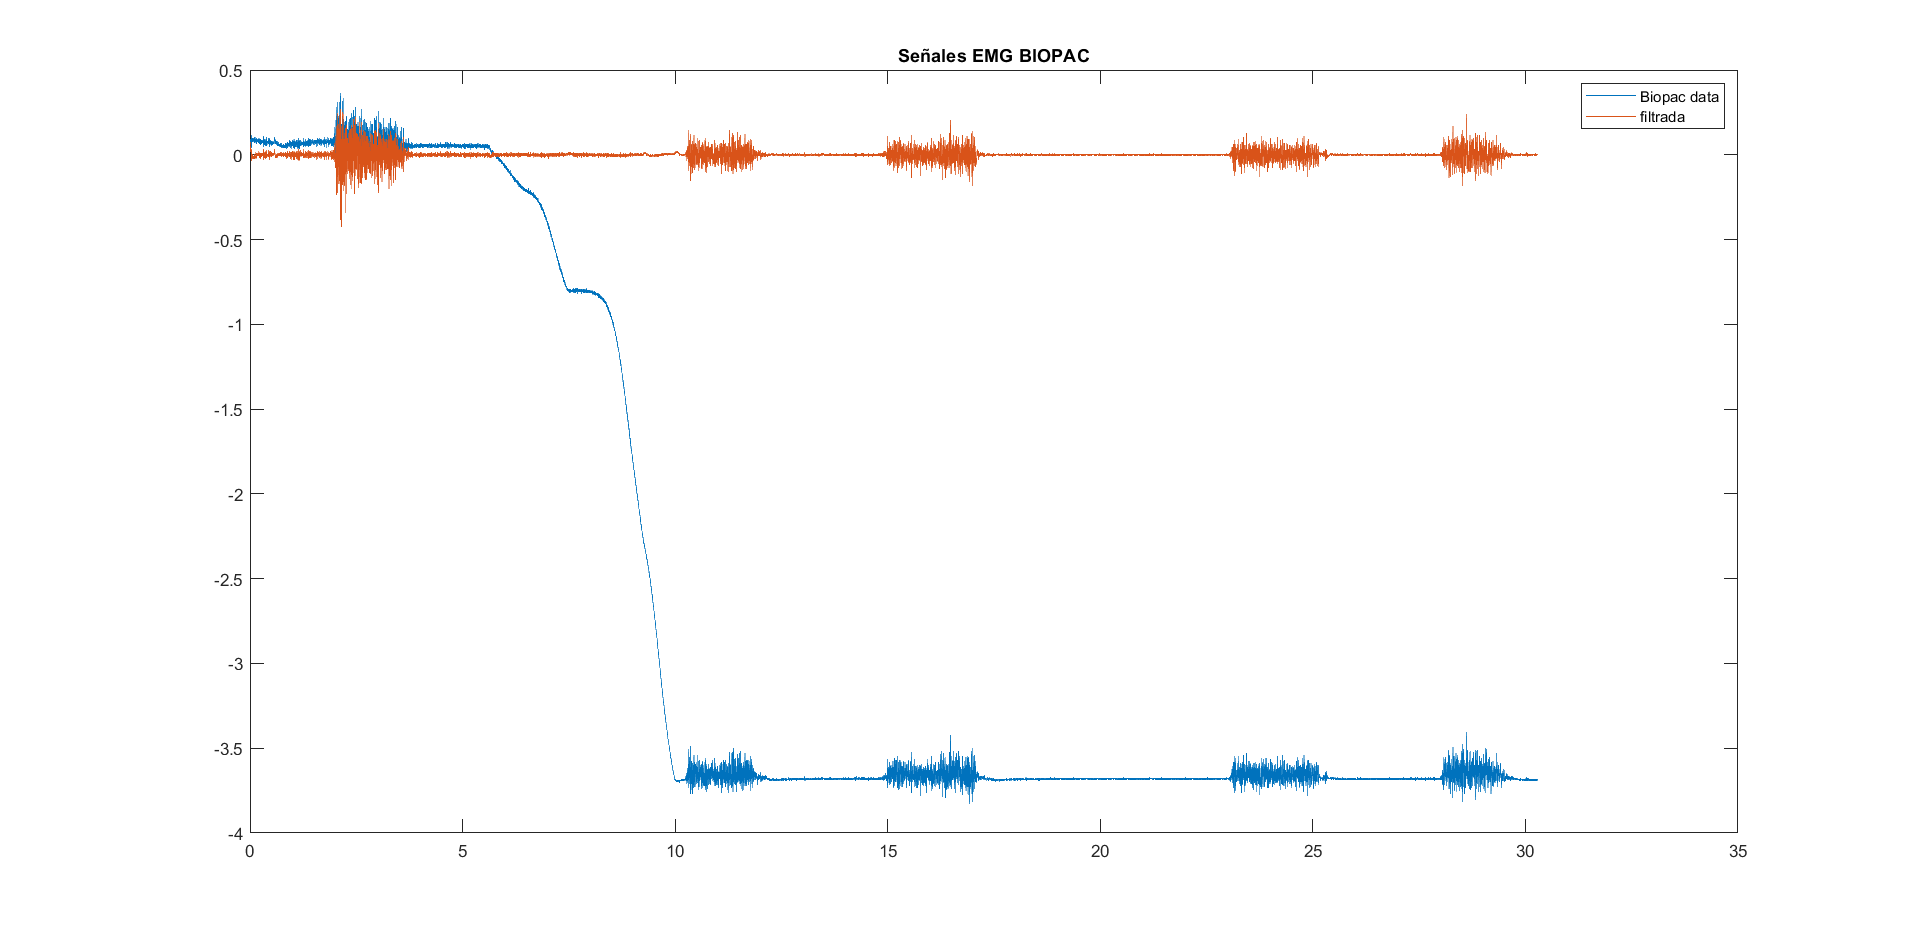
\includegraphics[width=0.9\textwidth]{figuras/10_filtro_MP41.png}
%    \caption{Señal original obtenido con MP41 (color azul) versus señal filtrada (color naranja).}
%    \label{fig:MP41_filtro}
%\end{figure}

\section{Datos obtenidos con equipo UVG}
En la Universidad del Valle de Guatemala se cuenta con los modelos MP36 y MP41 de BIOPAC, siendo el primero una versión más completa y de escritorio, mientras que el segundo es una versión portátil. Utilizando el equipo MP36 y MP41, se recopilaron señales del tipo EEG y EMG. Para cada tipo de señal bioeléctrica se tuvo un mínimo de tres sets diferentes de acciones por individuo.

\subsection{Señales EMG}
Para las señales EMG, el sujeto de prueba debía de encontrarse en estado de relajación. La pose del brazo en dicho estado se puede observar en la Figura~\ref{fig:relax_emg}.
Las grabaciones tuvieron una duración mínima de un minuto. Las personas mantuvieron la pose de relajación durante 2 segundos y posteriormente, durante otros 2 segundos realizaron la actividad solicitada, esto iteradas veces hasta cumplir con el mínimo de tiempo establecido. Las actividades fueron:

\begin{figure}[t]
    \centering
    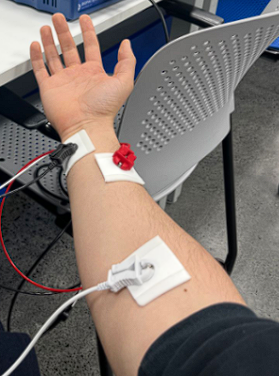
\includegraphics[width=0.2\textwidth]{figuras/16_emgRelax.png}
    \caption{Pose de relajación para toma de señales EMG con equipo BIOPAC.}
    \label{fig:relax_emg}
\end{figure}

\begin{figure}[t]
    \centering
    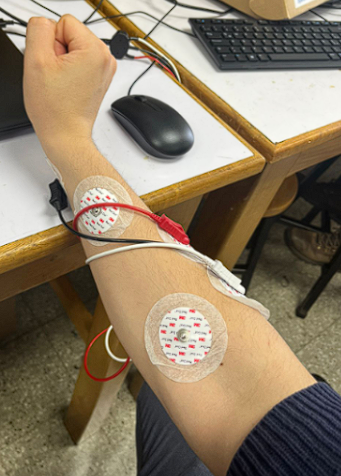
\includegraphics[width=0.2\textwidth]{figuras/17_elevarmunieca.png}
    \caption{Pose de actividad 1 en toma de grabación señal EMG.}
    \label{fig:actividad1_emg}
\end{figure}

\begin{figure}[H]
    \centering
    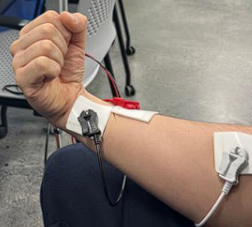
\includegraphics[width=0.2\textwidth]{figuras/19_contraer_munieca.png}
    \caption{Pose de actividad 2 en toma de grabación señal EMG.}
    \label{fig:actividad2_emg}
\end{figure}

\begin{figure}[H]
    \centering
    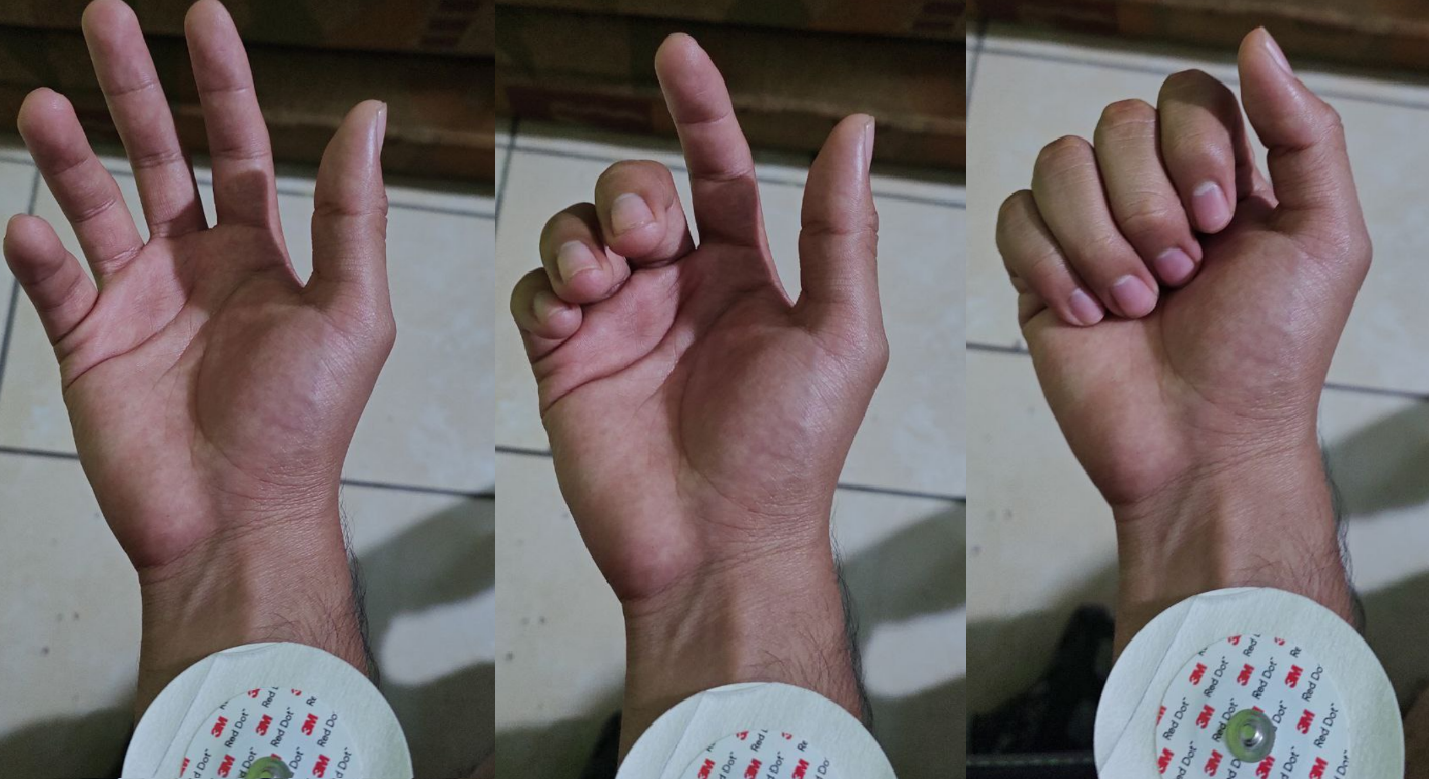
\includegraphics[width=0.3\textwidth]{figuras/18_empuniar.png}
    \caption{Pose de actividad 3 en toma de grabación señal EMG.}
    \label{fig:actividad3_emg}
\end{figure}

\begin{itemize}    
    \item Actividad 1:
    Elevar la muñeca hacia el exterior del cuerpo, como se observa en la Figura~\ref{fig:actividad1_emg}.    
    \item Actividad 2:
    Contraer la muñeca hacia el interior del cuerpo, como se observa en la Figura~\ref{fig:actividad2_emg}.     
    \item Actividad 3:
    Contraer paulatinamente cada uno de los dedos de la mano hacia el interior de la palma, como se observa en la Figura~\ref{fig:actividad3_emg}.    
\end{itemize}

\subsection{Señales EEG}
Para las señales EEG, el sujeto de prueba debía de encontrarse en estado de relajación, lo cual implicaba ojos cerrados y haber realizado al menos 3 repeticiones de inhalación y exhalación profundas.
Las grabaciones tuvieron una duración mínima de un minuto. Las personas mantuvieron la pose de relajación durante al menos 30 segundos al inicio, posteriormente se procedió a realizar una de las actividades especificas. Las actividades fueron:

\begin{itemize}    
    \item Actividad 1:
    Abrir los ojos durante 10 segundos y luego, volver a cerrar los ojos durante otros 10 segundo.   
    \item Actividad 2:
    Abrir los ojos y realizar una prueba matemática nivel medio, la cual consistía en sumas, restas, multiplicaciones y divisiones de números enteros de hasta 7 dígitos.
    \item Actividad 3:
    En los trabajos de graduación presentados por Margareth Vela \cite{magy_2023} y Oscar Fuentes \cite{oscar_2023}, los cuales consistieron en el estudio cualitativo y cuantitativo del impacto de los pulsos binaurales en el estado de ánimo, concentración y calidad del sueño de las personas y aplicación de técnicas de aprendizaje automático y reconocimiento de patrones en las señales bioeléctricas. Se realizaron las actividades 1 y 2 nuevamente pero ahora, mediante audífonos se aplicaron pulsos binaurales.
\end{itemize}

\subsection{Estándar en recolección de datos BIOPAC}
Se definió un documento estándar de formato ``.xlsx'' para el almacenamiento de las señales EMG y EEG obtenidas con el equipo BIOPAC,  como se observa en la Figura~\ref{fig:Estandar_bipoac_uvg}. Los datos principales que se necesitan son:

\begin{figure}[H]
    \centering
    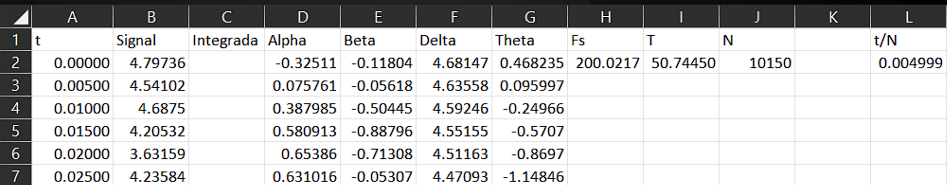
\includegraphics[width=0.9\textwidth]{figuras/11_estandar_biopac_uvg.png}
    \caption{Estándar para el almacenamiento de datos obtenidos con el equipo BIOPAC de la UVG.}
    \label{fig:Estandar_bipoac_uvg}
\end{figure}

\begin{itemize}
    \item Señal (signal)
    \item Tiempo de grabación (T)  
    \item Número de muestras (N)
\end{itemize}

La primer columna llamada ``t'' se auto genera al llenar los datos principales y consiste en el tiempo en el que se obtuvo la señal que se encuentra en la columna ``\textit{Signal}''. 
El parámetro que se encuentra en la columna ``Fs'' corresponde a la frecuencia de muestreo la cual se auto calcula.
El parámetro que se encuentra en la columna ``t/N'' corresponde al tiempo dividido numero de muestras la cual se auto calcula, esto permite marcar la diferencia de tiempo que hay entre una muestra y la siguiente.

Las columnas siguientes son opcionales ya que dentro de la herramienta de software para el estudio de la epilepsia no se hace uso de ellas. Por lo que siempre habrá al menos una de estas columnas en blanco, ya que se llenan acorde al tipo de señal bioeléctrica a recolectar. Estas columnas son:
\begin{itemize}
    \item Integrada: es el área situada bajo la curva de la señal EMG rectificada, lo que equivale a la integral matemática del valor absoluto de la señal EMG original \cite{BIOPAC}.
    \item Alpha: señal EEG filtrada para observar frecuencias de 8 Hz a 12 Hz.
    \item Beta: señal EEG filtrada para observar frecuencias de 12 Hz a 30 Hz.
    \item Delta: señal EEG filtrada para observar frecuencias de 1 Hz a 4 Hz.
    \item Theta: señal EEG filtrada para observar frecuencias de 4Hz a 8 Hz.
\end{itemize}


Tras recolectar estos datos la norma de almacenamiento consiste en, nombrar el documento con el nombre y apellido de la persona a la que se le extrajo las señales bioeléctricas, seguido de un guion (bajo o normal), el tipo de actividad que se realizó y por último, el tipo de señal bioeléctrica que se extrajo. En la Figura~\ref{fig:dataCruda_almacenada} se observa un ejemplo de ello.

\begin{figure}[H]
    \centering
    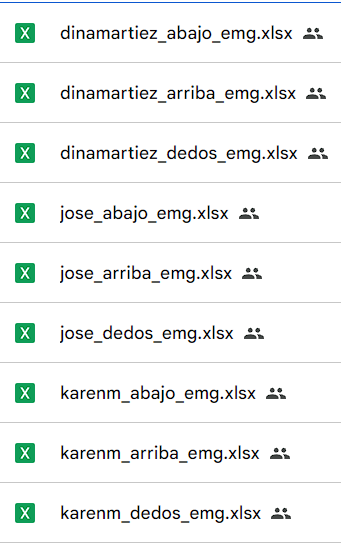
\includegraphics[width=0.30\textwidth]{figuras/20_datosCrudo_norma.png}
    \caption{Señales bioeléctricas extraídas con el equipo BIOPAC almacenadas según la norma establecida.}
    \label{fig:dataCruda_almacenada}
\end{figure}

\subsection{Estructuración de los datos para ser usados en la herramienta de software para el estudio de la epilepsia}
Para los datos obtenidos con el equipo BIOPAC de la UVG, es necesario convertirlos en un formato tipo \textit{Struct}, de esta manera se podrá usar dicha información dentro de la la herramienta de software para su análisis y estudio, como se muestra en la Figura~\ref{fig:struc_func}. 

\begin{figure}[H]
    \centering
    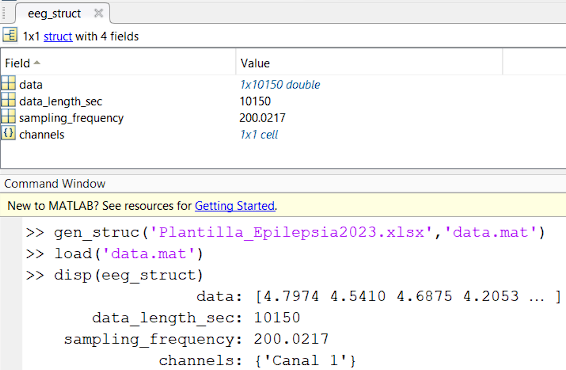
\includegraphics[width=0.6\textwidth]{figuras/12_struct_funct.png}
    \caption{Contenido de \textit{struct} para el uso de datos dentro de la herramienta de software para el estudio de la epilepsia.}
    \label{fig:struc_func}
\end{figure}

Para ello se creo la función ``gen\_struc'' la cual, posee como primer argumento el nombre del documento a extraer los datos y como segundo argumento el nombre y el formato con el que se almacenará el \textit{struct}. Dicho formato contiene los siguientes espacios:
\begin{itemize}
    \item Datos (mV)
    \item Cantidad de datos
    \item Frecuencia de muestreo (Hz)
    \item Cantidad de canales
\end{itemize}

\section{Datos de HUMANA de pacientes con epilepsia }
HUMANA ha compartido 4 grabaciones de señales EEG, la información de dichas grabaciones se puede ver en el Cuadro~\ref{cuadro:tabla_edf_info}. Estos datos fueron de ayuda para el entrenamiento y verificación de exactitud de los modelos de aprendizaje automático. 

\begin{table}[H]
\begin{center}    
    \begin{tabular}{|l|l|l|l|l|}
    \hline
    \multicolumn{1}{|c|}{\textbf{Nombre}} & \multicolumn{1}{c|}{\textbf{Canales}} & \multicolumn{1}{c|}{\textbf{Duración (HH:MM:SS)}} & \multicolumn{1}{c|}{\textbf{Frecuencia de muestreo}}\\ \hline
    AL.edf  & 33  & 03:01:56 & 200 Hz   \\ \hline
    CLEA.edf& 29  & 02:39:42 & 200 Hz   \\ \hline
    GIKA.edf& 29  & 02:58:06 & 200 Hz   \\ \hline
    HCHC.edf& 29  & 23:02:44 & 200 Hz   \\ \hline
    \end{tabular}
    \caption[Información de grabaciones dadas por HUMANA]{Información de grabaciones de señales bioeléctricas de pacientes con epilepsia brindadas por HUMANA.} 
    \label{cuadro:tabla_edf_info}
\end{center}
\end{table}

\section{Agrupamiento de datos}
Con el equipo UVG se recopilaron señales bioeléctricas del tipo EEG y EMG, las cuales se agruparon de forma intersujeto e intrasujeto respectivamente. En el caso de señales brindadas por HUMANA estas no necesitan agrupación, ya que por lo general son de una duración mayor a una hora de grabación contando como mínimo 29 canales, por lo que esto ya son datos suficientes para proceder a realizar su análisis.

El análisis de señales EEG de forma intersujeto y señales EMG de forma intrasujeto se realiza de esta manera debido a las diferencias fundamentales en la naturaleza de estas dos tipos de señales y los objetivos específicos de análisis en cada caso.

\subsection{Análisis de señales EEG de forma intersujeto}
Las señales EEG, que representan la actividad eléctrica del cerebro, tienden a mostrar una variabilidad significativa entre diferentes individuos. Las diferencias en la anatomía cerebral, la disposición de electrodos, la edad y otros factores pueden influir en las características de las señales EEG. Por lo tanto, se suele analizar de forma intersujeto para comprender cómo varían las respuestas entre diferentes personas.

El análisis intersujeto de las señales EEG es relevante en aplicaciones clínicas y de investigación que involucran poblaciones de pacientes o participantes diversos. Permite identificar patrones generales en grupos de personas y puede ayudar en la detección de trastornos neurológicos como la epilepsia en una población más amplia.

\subsection{Análisis de señales EMG de forma intrasujeto}
Las señales EMG, que registran la actividad eléctrica de los músculos, tienden a mostrar menos variabilidad intrasujeto, es decir, las características de la señal son relativamente consistentes en un individuo específico a lo largo del tiempo. Esto se debe a que la anatomía y la disposición de los músculos de una persona tienden a ser estables.


\section{Aprendizaje automático}
En la presente sección se presentan los algoritmos y métodos que se usaron para medir la efectividad de los algoritmos en el reconocimiento de patrones en señales bioeléctricas que sean de interés. 

\subsection{Extracción de características}
Se extrajo características en el dominio tiempo, frecuencia y wavelets, de cada uno de los datos obtenidos con el equipo UVG o brindados por HUMANA. Se analizó la generación de estas características, para optimizar el tiempo de entrenamiento de los algoritmos de aprendizaje automático y de ser posible la mejora de clasificación de las señales bioeléctricas.

\subsection{Anotaciones automáticas}
Empleando los algoritmos de aprendizaje automático desarrollados en las fases anteriores, se clasificó la señal bioeléctrica entre, ``Ictal'', ``Sano'', ``Interictal'' o Preictal'', según fuera su caso. A su vez, se implemento una sección para exportar los segmentos de interés a un documento CSV, como se puede observar en la Figura~\ref{fig:yo_anotaciones}.

\begin{figure}[H]
    \centering
    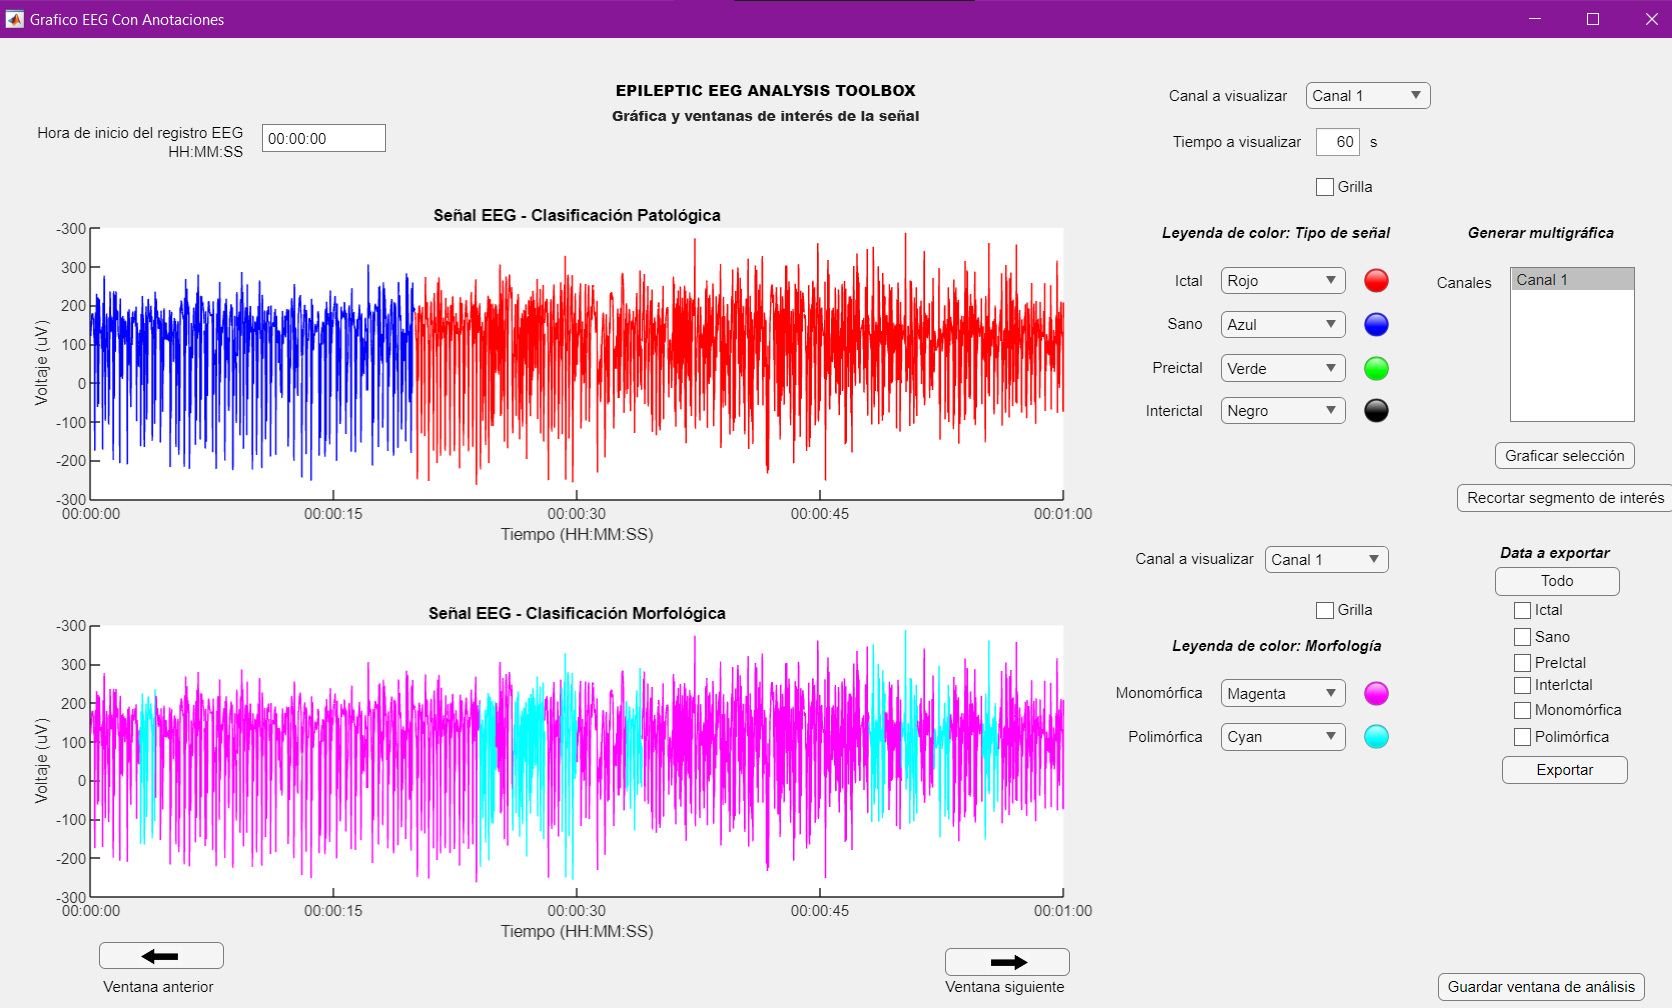
\includegraphics[width=0.6\textwidth]{figuras/13_modificacion_anotaciones.png}
    \caption{Ventana de anotaciones automáticas con nueva sección para exportar datos de interés.}
    \label{fig:yo_anotaciones}
\end{figure}

\subsection{Análisis estadístico}
Mediante matrices de confusión se validó la efectividad de las redes neuronales y las SVM (algoritmos de aprendizaje supervisado). Para el caso de los algoritmos de agrupamiento de \textit{K-means} y Jerárquico (algoritmos de aprendizaje no supervisado) se procedió a validar su efectividad mediante el algoritmo ``\textit{rand index}'', el cual es una medida de validez para algoritmos de agrupamiento. Además se tabularon tiempos relevantes, desde la extracción de características hasta la generación de anotaciones automáticas. 

\section{Actualización de la herramienta de software para el estudio de la epilepsia}
El primer paso para la actualización de la herramienta de software para el estudio de la epilepsia fue eliminar los mensajes de advertencia y arreglar errores que se encontraban dentro de la herramienta de software para el estudio de la epilepsia. En las Figuras~\ref{fig:yo_error_uno} y ~\ref{fig:yo_warning_uno} se puede observar algunos ejemplos, la mayoría de estos eran a causa de prácticas de programación no tan eficientes en MATLAB. 

\begin{figure}[t]
    \centering
    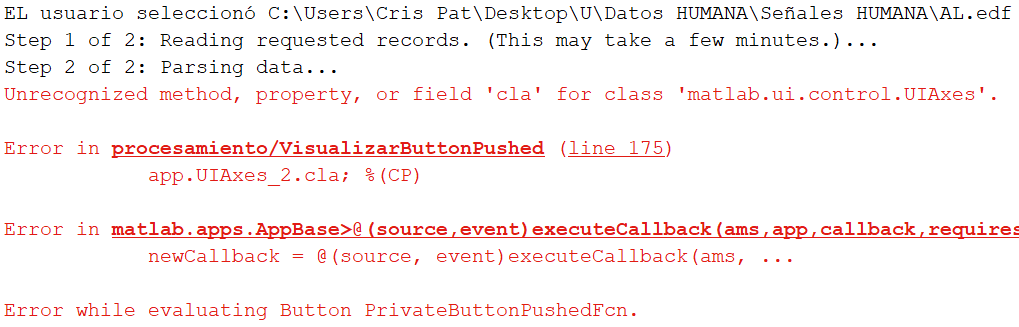
\includegraphics[width=0.65\textwidth]{figuras/14_AnalizaPrueba_visualizar.png}
    \caption{Error al utilizar botón de visualización de canales en la ventana de anotaciones automáticas.}
    \label{fig:yo_error_uno}
\end{figure}

\begin{figure}[t]
    \centering
    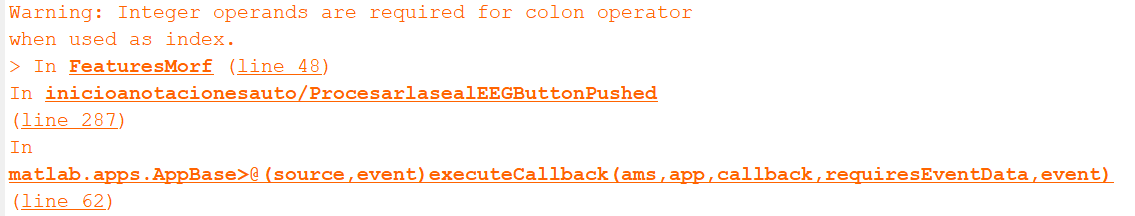
\includegraphics[width=0.65\textwidth]{figuras/15_alerta_feature_Morf.png}
    \caption{Alerta al emplear el algoritmo FeaturesMorf.}
    \label{fig:yo_warning_uno}
\end{figure}

\begin{figure}[t]
    \centering
    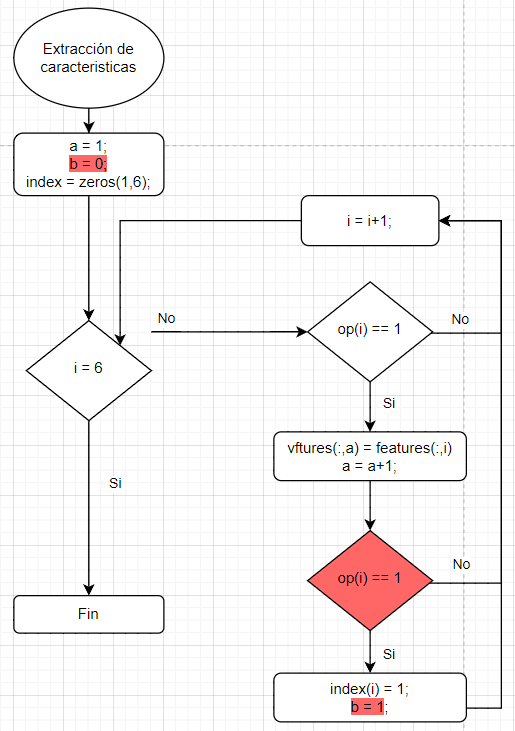
\includegraphics[width=0.40\textwidth]{figuras/21_flujograma_vfeatures_mal.png}
    \caption{Flujograma de la creación del vector de características versión 2022.}
    \label{flu:vfeatures malo}
\end{figure}

\begin{figure}[t]
    \centering
    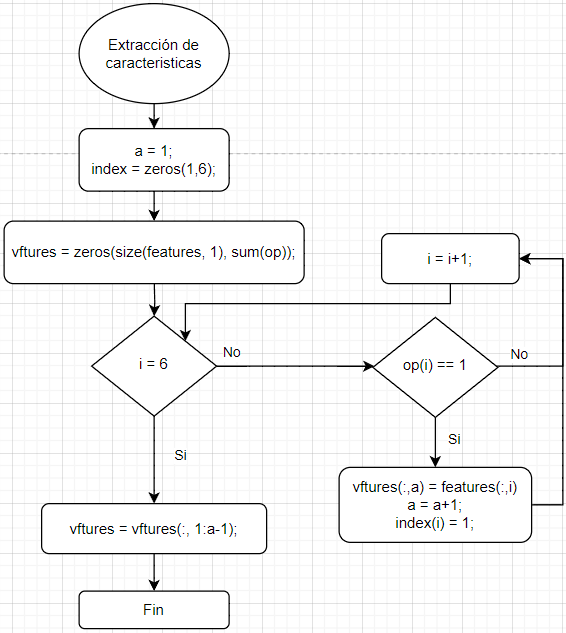
\includegraphics[width=0.45\textwidth]{figuras/22_flujograma_vfeatures_bien.png}
    \caption{Flujograma de la creación del vector de características versión 2023.}
    \label{flu:vfeatures bueno}
\end{figure}

En todos los casos al momento de extraer las características de las señales bioeléctricas, se tenía que no se pre-creaba el vector donde se almacenarían dichas características, además de contar con variables y condicionales innecesarias, como se puede observar en la Figura~\ref{flu:vfeatures malo}. Esto resulta ser computacionalmente costoso, lo que da paso a pérdida de tiempo innecesaria. Por lo que se procedió a corregirlo, creando el vector de características con las dimensiones máximas que podría tener, siendo la cantidad de filas del tamaño del vector de datos y la cantidad de columnas, del tamaño de las posibles características de interés, como se puede observar en la Figura~\ref{flu:vfeatures bueno}.

Al momento de establecer rangos de datos a analizar por ventanas, se encontraba como limite superior la expresión de la Ecuación(\ref{eq: Limite superior vfeatures}), lo cual al tratarse de un vector los valores ingresados para los índices deben ser enteros, característica que no cumple el limite superior cuando la variable ``muestras'' es un número impar. Por lo que se procedió a redondear el valor al mínimo más próximo, dando la expresión de la Ecuación(\ref{eq: vfeatures_rango}). Un claro ejemplo de este proceso se puede observar en la Figura~\ref{fig: redondeo minimo}. 

\begin{equation}
    Lim\_sup = \frac{muestras}{2} + 1
    \label{eq: Limite superior vfeatures}
\end{equation}

\begin{equation}
    VectorVentana=VectorAnalizar(1:floor( \frac{muestras}{2} + 1));
    \label{eq: vfeatures_rango}
\end{equation}

\begin{figure}[t]
    \centering
    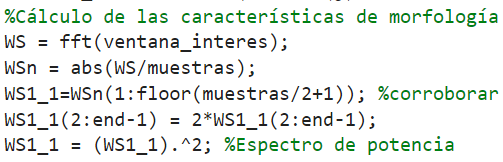
\includegraphics[width=0.45\textwidth]{figuras/23_redondeo_indicevector.png}
    \caption{Segmento de código para el calculo de características de una señal bioeléctrica.}
    \label{fig: redondeo minimo}
\end{figure}

En el proceso de generación de característica, el algoritmo para determinar el ``Zero Crossing'' (ZC) no era el más adecuado, dicho algoritmo se puede ver en la Figura~\ref{flu: ZC malo}. 
El algoritmo creaba variables que no se utilizaban, sin embargo, si se realizaban operaciones matemáticas con ellos, lo que implica tiempo y calculo computacional innecesario. A su vez, el algoritmo verificaba el cambio de signo directamente, sin usar el argumento ``umbral'', el cual es de gran relevancia ya que es este, quien permite el conteo adecuado de cambio de signo, sin tomar en cuenta aquellos cruces por cero que ocurren debido al ruido dentro de la señal. 
Por lo que se procedió a realizar las respectivas correcciones, como se muestra en la Figura~\ref{flu: ZC bueno}. En la presente versión se toma en cuenta el umbral para un correcto conteo, además de, ser una versión simplificada lo que lo hace más simple de realizar los cálculos computacionales.

\begin{figure}[t]
    \centering
    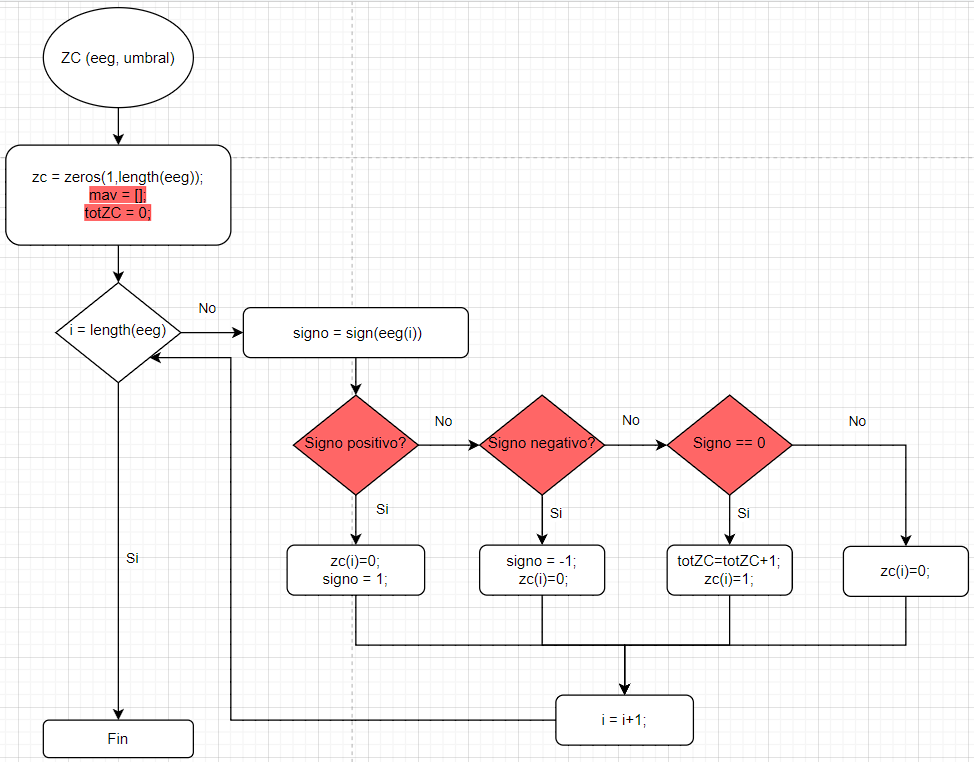
\includegraphics[width=0.7\textwidth]{figuras/24_flujograma_zc_mal.png}
    \caption{Flujograma de algoritmo ZC versión 2022.}
    \label{flu: ZC malo}
\end{figure}
\begin{figure}[t]
    \centering
    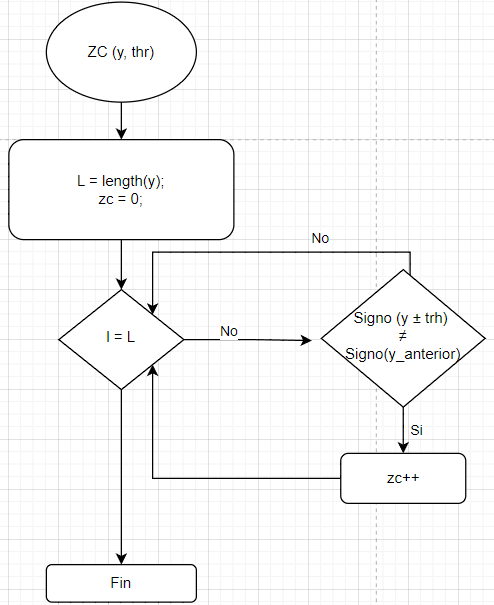
\includegraphics[width=0.4\textwidth]{figuras/25_flujograma_zc_bien.png}
    \caption{Flujograma de algoritmo ZC versión 2023.}
    \label{flu: ZC bueno}
\end{figure}

%-------------------------------------------------------
% A partir de aqui se discuten los resultados
%-------------------------------------------------------
\chapter{Resultados de recolección de datos}
En el presente capitulo se presentarán los datos de señales bioeléctricas obtenidas con el equipo de UVG y brindadas de HUMANA. Estas señales fueron la materia prima para la comprobación de funcionalidad de los algoritmos.

\section{Señales Bioeléctricas obtenidas con el equipo de UVG}
La recolección de señales bioeléctricas con el equipo de UVG ha dado como resultado un total de 60 grabaciones, como se puede ver en el Cuadro~\ref{cuadro:tabla datos UVG}. Para el caso de las señales EEG, se cuenta con una duración promedio de 20 minutos por grabación. En el caso de las señales EMG, se cuenta con una duración promedio de 1 minuto por grabación. Por lo que ahora se cuenta con una base de datos de Señales EEG y EMG, recolectadas y procesadas en la Universidad del Valle de Guatemala.

En el Cuadro \ref{cuadro:tabla datos UVG} de datos recolectados, la categoría ``sin plantilla'' se refiere a grabaciones de señales bioeléctricas que no se guardaron con el ``Estándar en recolección de datos BIOPAC'', mientras que la categoría ``con plantilla'' hace referencia a grabaciones de señales bioeléctricas que sí utilizaban dicho estándar. 

\begin{table}[H]
\begin{center}
    \begin{tabular}{|l|l|l|l|l|}
    \hline
        \multicolumn{1}{|c|}{\textbf{Tipo}} & \multicolumn{1}{c|}{\textbf{Cantidad}} & \multicolumn{1}{c|}{\textbf{Formato}}\\ \hline
        EEG sin plantilla & 12  & XLSX \\ \hline
        EEG con plantilla & 0  & No aplica \\ \hline
        EMG sin plantilla & 12  & XLSX \\ \hline
        EMG con plantilla & 36  & XLSX \\ \hline
    \end{tabular}
    \caption[Datos en nube con equipo UVG]{Datos recolectados con equipo UVG.} 
    \label{cuadro:tabla datos UVG}
\end{center}
\end{table}

Una vez organizado los datos obtenidos con el equipo de UVG, se procedió a generar los \textit{structs}, ya que este formato es el utilizado en la herramienta de software para el estudio de la epilepsia, siguiendo la norma que se describió en el capitulo anterior se almacenaron, se puede observar en la Figura~\ref{fig: Struct_normado}. Este formato permite extraer características de las grabaciones realizadas.

\begin{figure}[t]
    \centering
    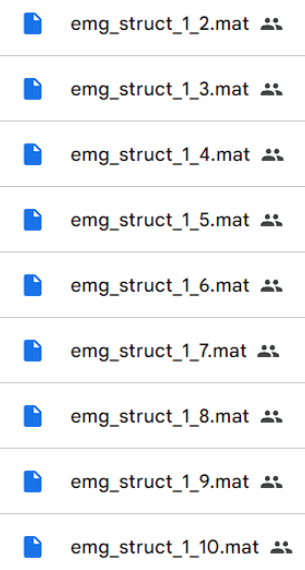
\includegraphics[width=0.15\textwidth]{figuras/29_strucs_normados.png}
    \caption{Structs generados a partir de los datos obtenidos con el equipo UVG.}
    \label{fig: Struct_normado}
\end{figure}

\subsection{Resultados de la Extracción de Características}
Para los datos recolectados se procedió a extraer sus características. Cabe mencionar que los datos que se obtuvieron con el equipo UVG son de personas que no padecen de epilepsia, teniendo un total de 10 vectores de características y 24 \textit{structs}, como se observa en el Cuadro~\ref{cuadro:tabla datos features UVG}.

\begin{table}[H]
\begin{center}
    \begin{tabular}{|l|l|l|l|l|}
    \hline
        \multicolumn{1}{|c|}{\textbf{Tipo}} & \multicolumn{1}{c|}{\textbf{Cantidad}} & \multicolumn{1}{c|}{\textbf{Formato}}\\ \hline
        \textit{Struct} de datos con señales bioeléctricas & 24  & MAT \\ \hline
    \end{tabular}
    \caption[Datos procesados en nube con equipo UVG]{Datos procesados de las grabaciones que se recolectaron con equipo UVG.} 
    \label{cuadro:tabla datos features UVG}
\end{center}
\end{table}

Para la generación de los vectores de características se cargaron solo 2 sets de datos, los de HUMANA tienen segmentos ictales (crisis) y no ictales (no crisis).
Posteriormente se procedió a generar los vectores de características en tiempo continuo y wavelets, con todas las características seleccionadas, como se puede ver en las Figuras~\ref{fig: carac_tiempo} y \ref{fig: carac_wavelets}. Considerando que las grabaciones de HUMANA tienen una duración mayor a 2 horas, como se observa en el Cuadro~\ref{cuadro:tabla_edf_info}, los tiempos en los que se extrajo las características fue favorable, como se puede ver en el Cuadro~\ref{cuadro:Duracion caracteristicas}. 

\begin{figure}[H]
    \centering
    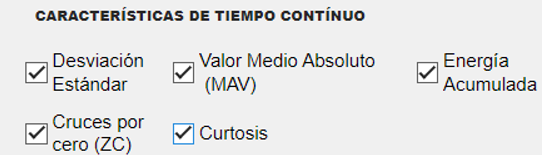
\includegraphics[width=0.4\textwidth]{figuras/26_carac_tiempo.png}
    \caption{Características en el dominio del tiempo continuo.}
    \label{fig: carac_tiempo}
\end{figure}

\begin{figure}[H]
    \centering
    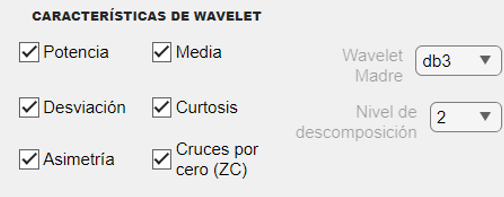
\includegraphics[width=0.4\textwidth]{figuras/27_carac_wavelet.png}
    \caption{Características con wavelets.}
    \label{fig: carac_wavelets}
\end{figure}

En cuanto a las características en el dominio de la frecuencia, la primera corrida se intento recolectar todas las características a la vez, como se puede observar en la Figura~\ref{fig: carac_freq}; pero el proceso se interrumpió al transcurrir las 6 horas y no finalizar. Por lo que se procedió a extraer las características una a la vez, obteniendo periodos de duración muy grandes en comparación a las características en el dominio del tiempo y wavelets. 

\begin{figure}[H]
    \centering
    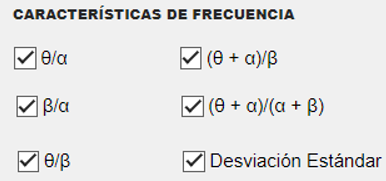
\includegraphics[width=0.4\textwidth]{figuras/28_carac_freq.png}
    \caption{Características en el dominio de la frecuencia.}
    \label{fig: carac_freq}
\end{figure}

\begin{table}[H]
\begin{center}
\begin{tabular}{|l|l|l|l|l|}
\hline
        \multicolumn{1}{|c|}{\textbf{Tipo}} &
   \textbf{ Hora inicio (hh:mm:ss)} & \textbf{Hora fin (hh:mm:ss)} & \textbf{Duración (hh:mm:ss)}   \\ \hline
    Tiempo continuo     & 14:54:00  & 15:33:07 & 00:39:07   \\ \hline
    Wavelet             & 15:35:00  & 15:35:32 & 00:00:32   \\ \hline
    Frecuencia          & 11:18:00  & 11:09:32 & 23:50:28   \\ \hline
    $\theta/\alpha$     & 17:10:25  & 18:26:52 & 01:16:27   \\ \hline
    $\beta/\alpha $     & 18:30:00  & 19:34:27 & 01:04:27   \\ \hline
    $\theta/\beta $     & 19:38:00  & 20:44:07 & 01:06:07   \\ \hline
\end{tabular}
\caption[Tiempos de extracción de características]{Tiempos de extracción de características con señales de HUMANA y UVG.} 
\label{cuadro:Duracion caracteristicas}
\end{center}
\end{table}

\section{Anotaciones automáticas}
El espacio de anotaciones automáticas necesita ser cargado con un set de datos provenientes de una señal bioeléctrica; un clasificador el cuál es el encargado de segmentar y así poder diferenciar el tipo de estado en el que se encuentra el paciente (Sano, ictal, preictal, interictal) y posteriormente se debe seleccionar los canales a analizar, como se observa en la Figura~\ref{fig: pre_anotaciones_ventana}. 

\begin{figure}[H]
    \centering
    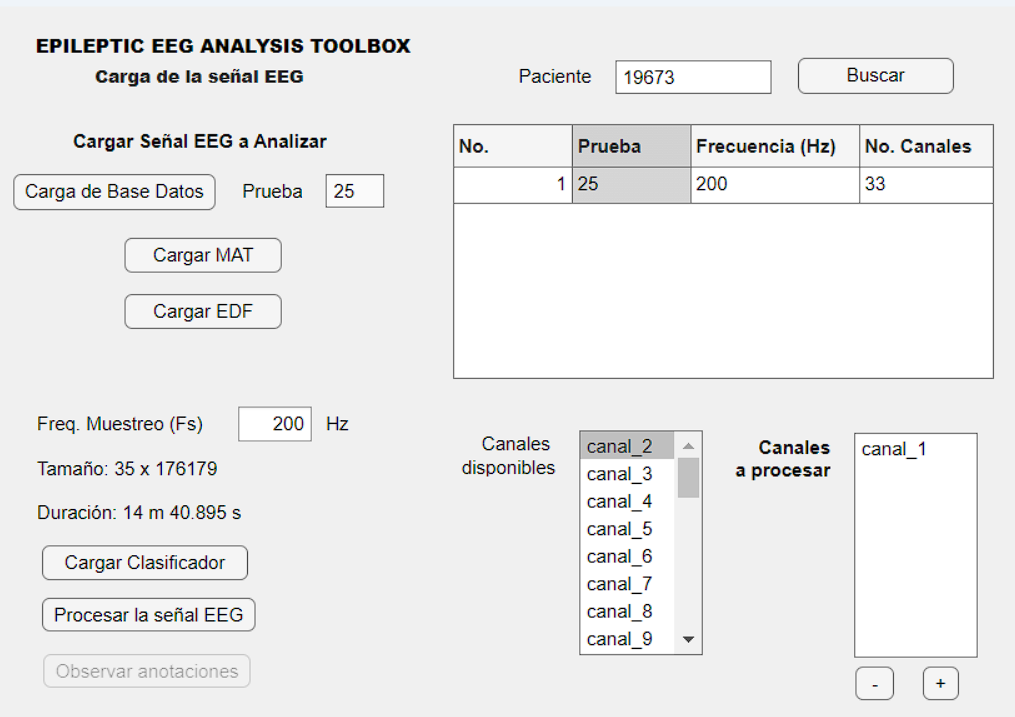
\includegraphics[width=0.6\textwidth]{figuras/31_ventana_preAnotaciones.png}
    \caption{Ventana de inicio para generar anotaciones automáticas.}
    \label{fig: pre_anotaciones_ventana}
\end{figure}

Para lo que se procedió a comprobar los tiempos de anotación según el clasificador, como se aprecia en el Cuadro~\ref{cuadro:Duracion anotaciones}. Como se puede observar nuevamente las wavelets son las características de menos duración, en este caso para la generación de anotaciones. 

\begin{table}[H]
\begin{center}
\begin{tabular}{|l|l|l|l|l|}
\hline
    \multicolumn{1}{|c|}{\textbf{Clasificador}} & \multicolumn{1}{c|}{\textbf{Duración (hh:mm:ss)}} & \multicolumn{1}{c|}{\textbf{Grabación }} \\ \hline
    RNA Tiempo   & 01:27:00  & AL.edf   \\ \hline
    RNA Frecuencia& 01:07:00  & AL.edf   \\ \hline
    RNA Wavelet   & 00:12:00  & AL.edf   \\ \hline
\end{tabular}
\caption[Tiempos de entrenamiento para clasificadores]{Tiempos de entrenamiento para clasificadores con señales bioeléctricas de HUMANA y UVG.} 
\label{cuadro:Duracion anotaciones}
\end{center}
\end{table}

En las Figuras~\ref{fig: 33_chn_grafica} y \ref{fig: 33_chn_grafica_menos}, se observa la misma grabación brindada por HUMANA, la cual trata de una persona que tuvo iteradas ocasiones episodios epilépticos. La razón por la que visualmente difiere una de la otra es debido a la clasificación realizada, de lo cual se habla en los párrafos siguientes. 

En la grabación de las Figuras~\ref{fig: 33_chn_grafica} y \ref{fig: 33_chn_grafica_menos}, se percibe cambios abruptos, lo cual permite una diferencia visual de segmentos. Los segmento donde se encuentra una mayor densidad de oscilaciones y altas amplitudes (visualmente segmento más grueso), se debe a disparos de actividad bioeléctrica en el cerebro más movimiento físico debido a una convulsión. En cuanto a los segmento donde se percibe menos oscilaciones a una baja amplitud, son segmentos donde la persona no se encuentra en actividad ictal.  

Es en esta parte donde se puede notar la necesidad de una mayor cantidad de señales bioeléctricas por parte de HUMANA, ya que en la Figura~\ref{fig: 33_chn_grafica}, se muestra el resultado para la generación de anotaciones automáticas. Es casi nulo a simple vista, los segmentos que marcan actividad ictal (color rojo) versus los segmentos en estado sano (color azul). Esto en gran medida se debe a un fuerte sesgo de una mayor cantidad de datos EEG de personas sanas, que de personas con episodios epilépticos. 

\begin{figure}[H]
    \centering
    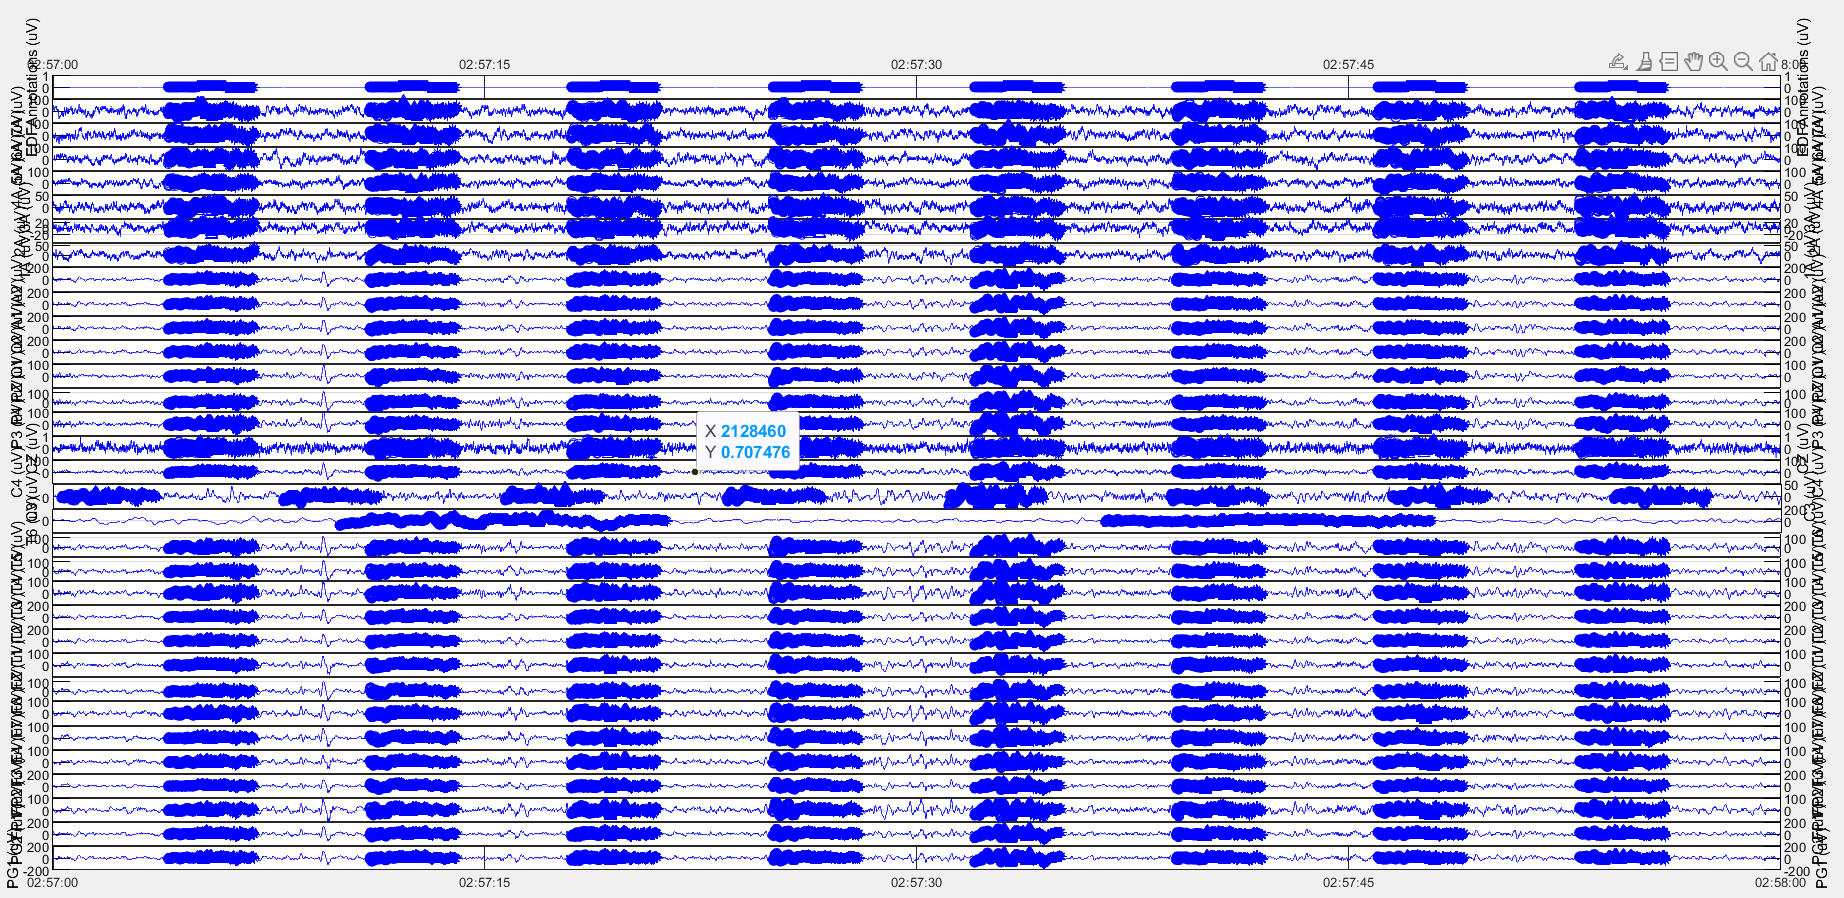
\includegraphics[width=0.77\textwidth]{figuras/30_33_canales_edf_humana.png}
    \caption{Anotaciones automáticas de 33 canales analizados.}
    \label{fig: 33_chn_grafica}
\end{figure}

Para solventar el inconveniente anterior sin contar con más datos por parte de HUMANA, se entreno al modelo con una menor cantidad de datos de personas sin actividad epiléptica. Desafortunadamente el resultado no fue el esperado. Como se puede observar en la Figura~\ref{fig: 33_chn_grafica_menos}, ahora se contaba con el inconveniente que era mayor el sesgo por los datos de actividad epiléptica respecto a los segmentos en estado sano.

\begin{figure}[H]
    \centering
    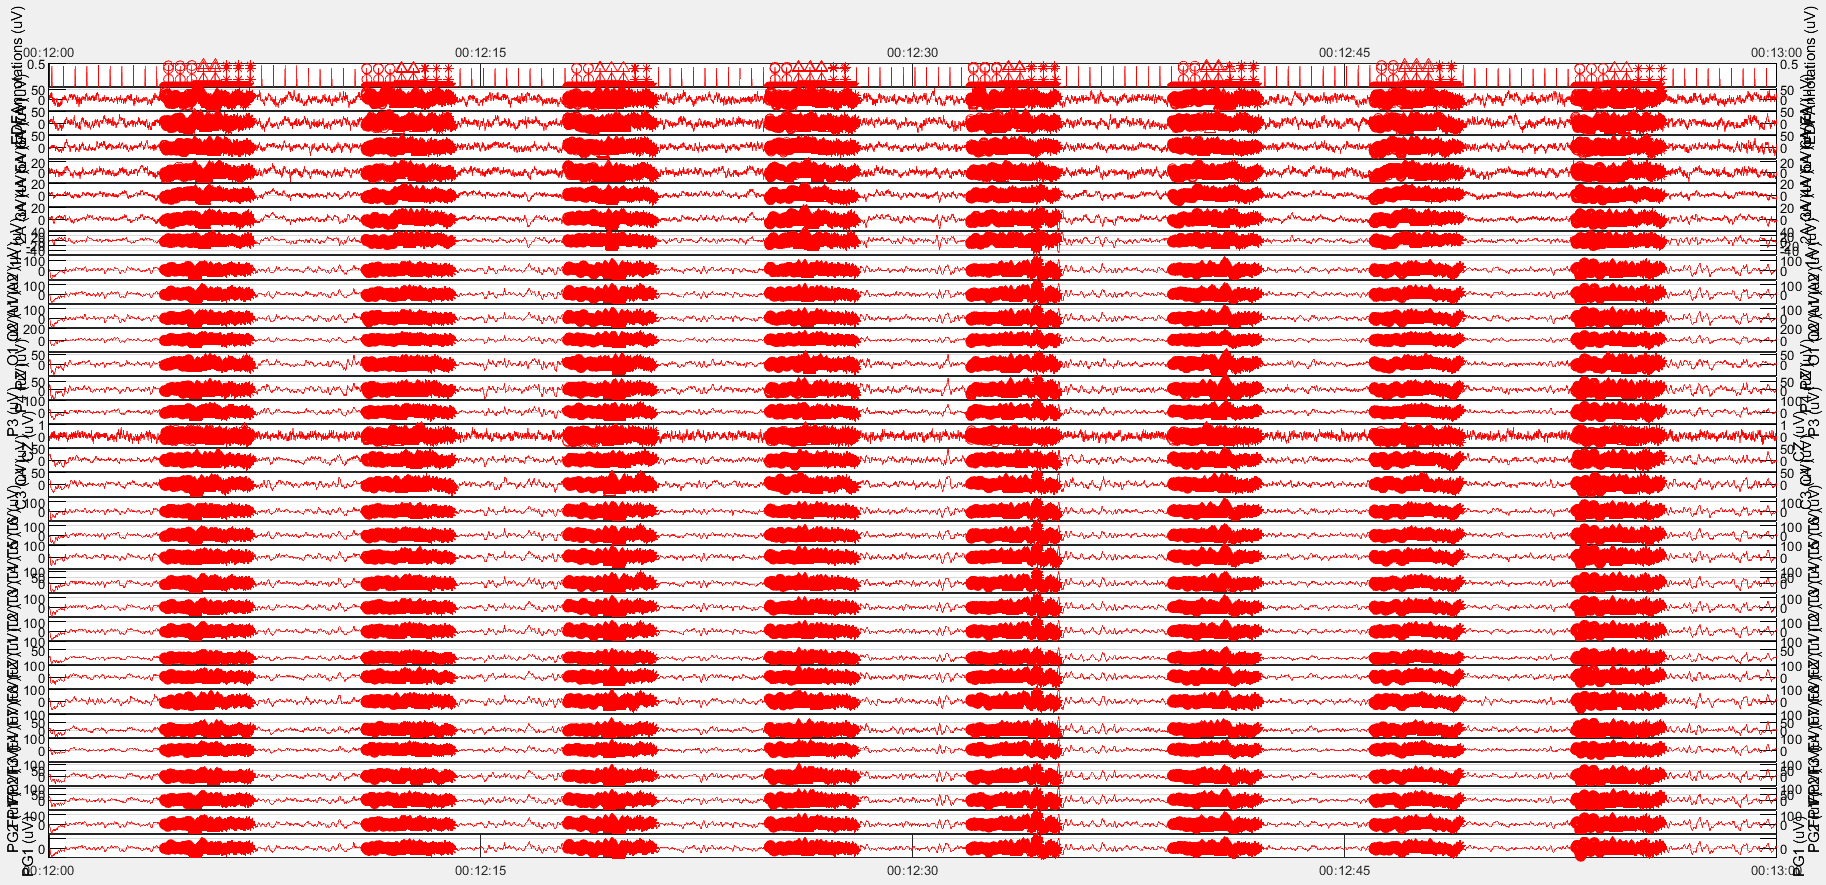
\includegraphics[width=0.77\textwidth]{figuras/33_33_canales_wavelet_edf_humana.png}
    \caption{Anotaciones automáticas de 33 canales analizados con menor cantidad de EEG de personas sin actividad ictal.}
    \label{fig: 33_chn_grafica_menos}
\end{figure}

Para solucionar este inconveniente, lo adecuado será entrenar el modelo con la misma cantidad de datos de señales bioeléctricas, además de, contar con la misma cantidad de personas sanas y personas con episodios epilépticos de las que se extraen las señales bioeléctricas. Esto permitirá al modelo encontrar las características necesarias de cada estado de interés, sin importar el sujeto. Ya que actualmente el modelo es preciso solo con las mismas personas con las que se entreno el modelo. Esto quiere decir que la predicción del modelo se ve afectada si, las señales bioeléctricas provienen de personas distintas de las que se obtuvieron los datos con los que se entrenó el modelo. 

\chapter{Resultados estadísticos}
En este capítulo, se presentan los resultados estadísticos obtenidos a partir de la aplicación de diversos métodos de análisis en el estudio de las señales bioeléctricas. Se analizan los resultados de los clasificadores empleados, se presentan las matrices de confusión que reflejan la capacidad de predicción, y se evalúan los resultados de los algoritmos de \textit{clustering} mediante el algoritmo \textit{rand index}.

\section{Clasificadores}
Los clasificadores empleados para esta etapa mediante aprendizaje supervisado fueron las RNA y las SVM, dando resultados positivos. 

Las SVM presentaron una mejor clasificación de los segmentos de las  señales bioeléctricas, como se puede observar en las Figuras~\ref{fig: Matriz confusion svm wavelets}, \ref{fig: Matriz confusion svm time} y  \ref{fig: Matriz confusion svm freq}. Estando por encima de un 85\% de exactitud. Presentando que las características de mejor comportamiento para clasificación son las  ``wavelets'' seguidas de las características de ``tiempo continuo'' y por ultimo las características de ``frecuencia''.

Las RNA por su parte, también produjeron resultados positivos con ligera diferencia respecto a las SVM, como se puede observar en las Figuras~\ref{fig: Matriz confusion RNA wavelet}, \ref{fig: Matriz confusion RNA tiempo} y \ref{fig: Matriz confusion RNA freq}. Las cuales también se encuentran por encima del 85\% de exactitud. Se percibe nuevamente que las mejores características para la clasificación de señales bioeléctricas son ``wavelets'', en cuanto a las  características de ``tiempo continuo'' se nota una perdida del 0.4\% de exactitud respecto a la clasificación por SVM y una perdida del 0.2\% de exactitud empleando las características de ``frecuencia'' respecto a la clasificación por SVM.

\begin{figure}[H]
    \centering
    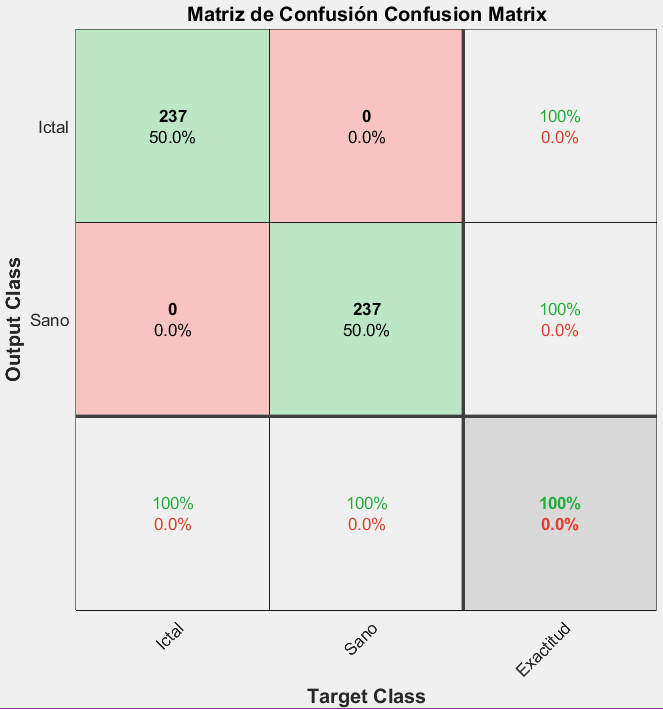
\includegraphics[width=0.5\textwidth]{figuras/37_svm_wavelet_edf_15ubon.png}
    \caption{Matriz de confusión para las clases Ictal y Sano utilizando SVM con características wavelets.}
    \label{fig: Matriz confusion svm wavelets}
\end{figure}
\begin{figure}[H]
    \centering
    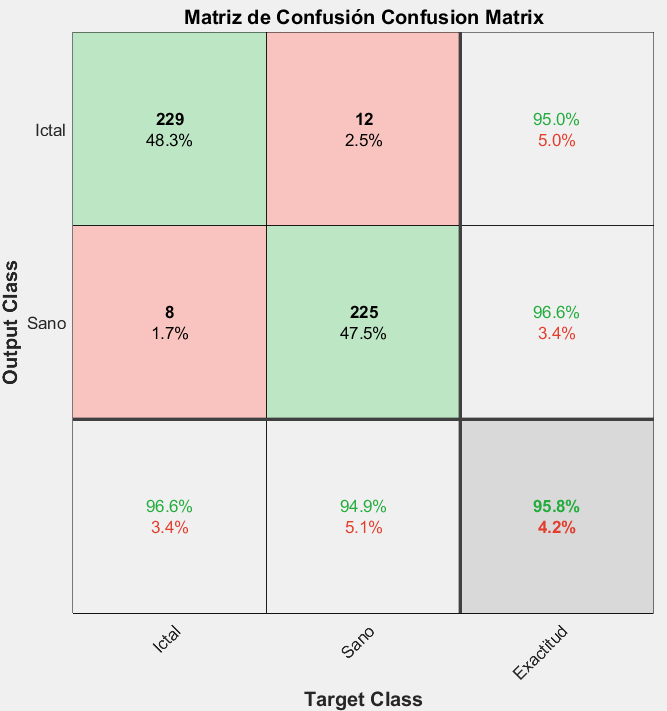
\includegraphics[width=0.5\textwidth]{figuras/38_svm_time_edf_15ubon.png}
    \caption{Matriz de confusión para las clases Ictal y Sano utilizando SVM con características en tiempo continuo.}
    \label{fig: Matriz confusion svm time}
\end{figure}
\begin{figure}[H]
    \centering
    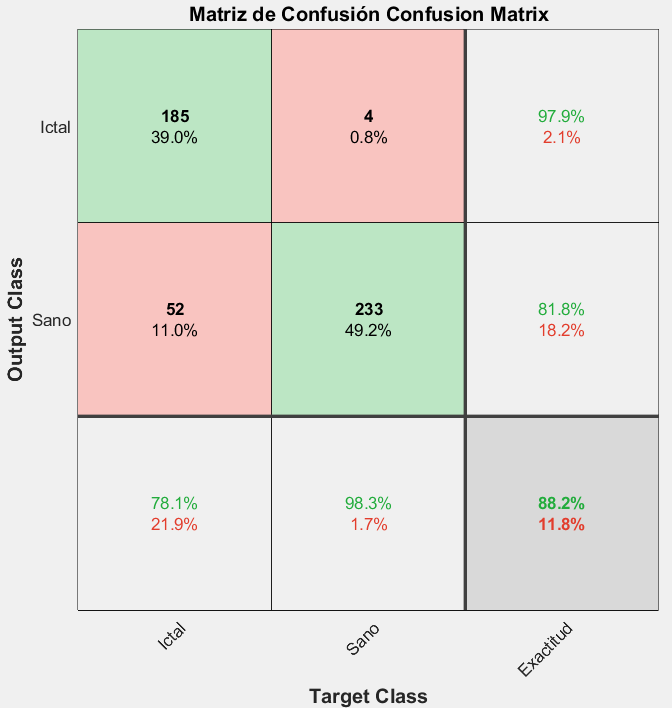
\includegraphics[width=0.5\textwidth]{figuras/36_svm_freq_edf_15ubon.png}
    \caption{Matriz de confusión para las clases Ictal y Sano utilizando SVM con características frecuencia.}
    \label{fig: Matriz confusion svm freq}
\end{figure}

\begin{figure}[H]
    \centering
    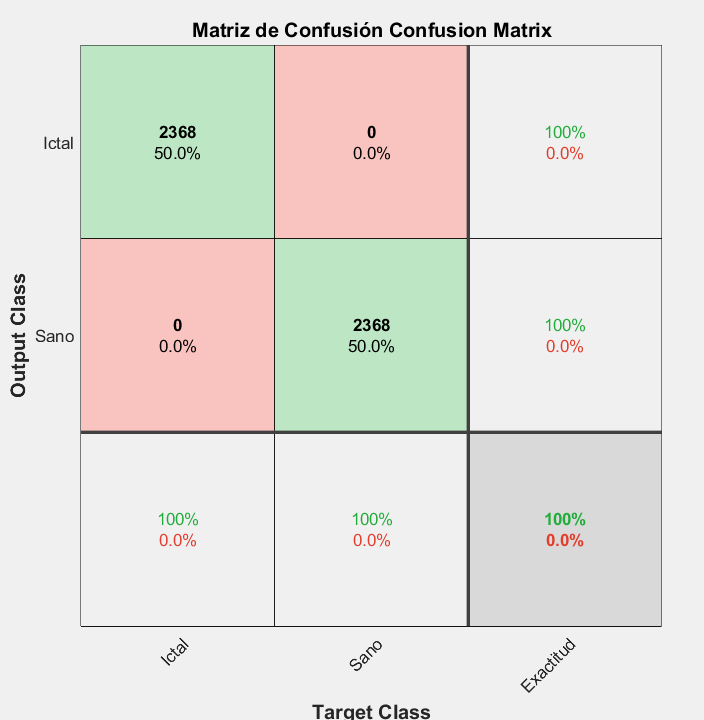
\includegraphics[width=0.5\textwidth]{figuras/32_rnn_wavelet_edf_15ubon.png}
    \caption{Matriz de confusión para las clases Ictal y Sano utilizando RNA con características wavelets.}
    \label{fig: Matriz confusion RNA wavelet}
\end{figure}
\begin{figure}[H]
    \centering
    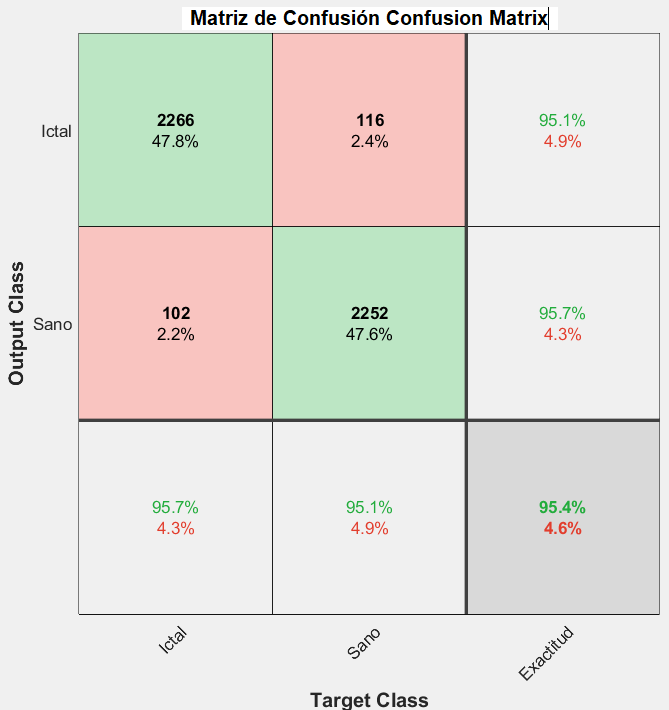
\includegraphics[width=0.5\textwidth]{figuras/34_rnn_tiempo_edf_15ubon.png}
    \caption{Matriz de confusión para las clases Ictal y Sano utilizando RNA con características en tiempo continuo.}
    \label{fig: Matriz confusion RNA tiempo}
\end{figure}
\begin{figure}[H]
    \centering
    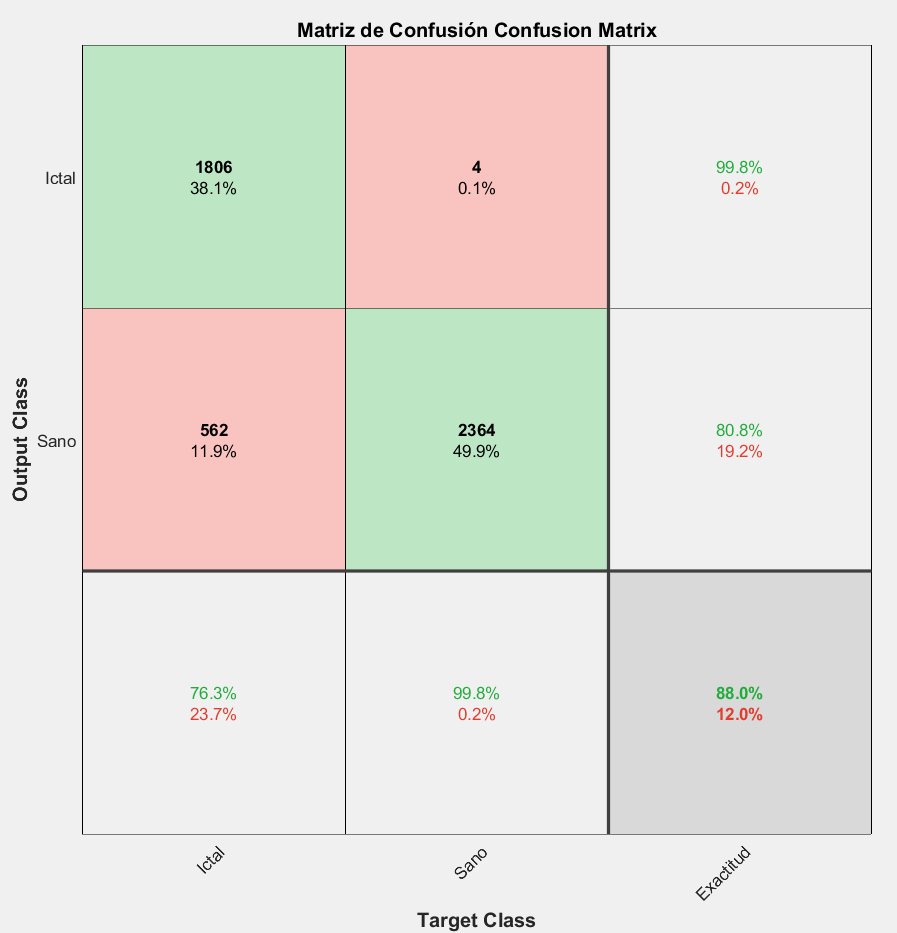
\includegraphics[width=0.55\textwidth]{figuras/35_rnn_freq_edf_15ubon.png}
    \caption{Matriz de confusión para las clases Ictal y Sano utilizando RNA con características en frecuencia.}
    \label{fig: Matriz confusion RNA freq}
\end{figure}

\section{Algoritmos de agrupamiento}
Los algoritmos de agrupamiento empleados para esta etapa mediante aprendizaje no supervisado fueron \textit{K-means} y jerárquico, obteniendo resultados positivos. 

Como se puede observar en el Cuadro~\ref{cuadro:resultado rand index}, las características ``wavelets'' y ``tiempo continuo'' independientemente del algoritmo de agrupación se obtienen los mismos resultados, sin embargo, para  las características de ``frecuencia'' si se nota una gran mejora de clasificación con el algoritmo de agrupamiento jerárquico dando un 30.46\% de superioridad versus el algoritmo de agrupamiento \textit{K-means}.

Por lo que nuevamente las características ``wavelets'' son las que presentan mejores resultado para la clasificación de segmentos de interés en señales bioeléctricas. Para las características en ``tiempo continuo'' se puede mejorar el porcentaje de clasificación obteniendo una mayor cantidad de características. En cuanto a las características de ``frecuencia'' si es notorio una mejora para el algoritmo de agrupamiento jerárquico. Las características en el dominio de la frecuencia a menudo tienen una estructura más jerárquica y pueden exhibir patrones de similitud a diferentes escalas. El agrupamiento jerárquico se adapta bien a la estructura jerárquica de los datos y puede identificar grupos en diferentes niveles de detalle, lo que puede ser beneficioso en datos con patrones complejos.

\begin{table}[H]
\begin{center}
    \begin{tabular}{|l|l|r|}
    \hline
        \multicolumn{1}{|c|}{\textbf{Algoritmo de agrupamiento}} & \multicolumn{1}{c|}{\textbf{Característica}} & \multicolumn{1}{c|}{\textbf{Rand index}}\\ \hline
        K-means  & Wavelets &  100.00\% \\ \hline
        K-means  & Tiempo continuo & 70.68\% \\ \hline
        K-means  & Frecuencia & 50.01\% \\ \hline
        Jerárquico & Wavelets &  100.00\% \\ \hline
        Jerárquico & Tiempo continuo & 70.68\% \\ \hline
        Jerárquico & Frecuencia & 91.55\% \\ \hline
    \end{tabular}
    \caption[Resultado rand index para algoritmos de agrupamiento]{Porcentaje de validación para los algoritmos de agrupamiento mediante \textit{rand index}.} 
    \label{cuadro:resultado rand index}
\end{center}
\end{table}

\chapter{Análisis de grupos}
El análisis de grupos (\textit{clustering}) desempeña un papel fundamental en la investigación, ya que permite explorar la estructura subyacente de las señales bioeléctricas recopiladas. En este capítulo, se presentan los resultados del uso de algoritmos de agrupamiento, en particular el método de K-means, aplicados a las señales bioeléctricas en diferentes dominios: tiempo, frecuencia y wavelets. Cabe mencionar que los datos utilizados son el resultado de una época de 0.4 segundos, por lo que la densidad de muestras cambiara según la frecuencia con la que se haya grabado la señal bioeléctrica para las clases ictal, sano, preictal e interictal.
%revisar app "generacionesalgoritmo.mlapp" linea 323, variable "app.s_ventana"

La agrupación de señales bioeléctricas es esencial para identificar patrones, tendencias y características comunes en los datos. Al aplicar K-means en distintos dominios, se exploran las similitudes y diferencias en la estructura de las señales, lo que permite obtener una visión más completa de los conjuntos de datos.

Los resultados presentados en las figuras se derivan de un enfoque de características a pares, lo que se justifica por la complejidad visual asociada al uso de K-means con un conjunto de características que excede las tres dimensiones. Esta estrategia permite una representación más clara y manejable de los datos, facilitando la identificación y análisis de patrones en las señales bioeléctricas.

\section{Análisis de Grupos en el Dominio de Tiempo}
En esta sección, se presenta el análisis de grupos aplicado a las características extraídas en el dominio del tiempo. 
Las características que se extrajeron en el dominio del tiempo fueron:
\begin{enumerate}
    \item Desviación estándar
    \item Valor medio absoluto (MAV)
    \item Cruces por cero (ZC)
    \item Curtosis
    \item Energía acumulada
\end{enumerate}

Los resultados del proceso de agrupamiento en el dominio de tiempo revelan una interesante distribución de los datos. En particular,como se observa en las Figuras~\ref{fig: k_means_Time_1_2} y \ref{fig: k_means_time_1_4} la distribución de los datos son muy continuos, lo cual indica que las características 1 respecto de 2 y 1 respecto de 4 podrían no ser muy efectivas para la predicción del tipo de señal bioeléctrica. Mientras que en las Figuras ~\ref{fig: k_means_time_1_5}, \ref{fig: k_means_time_2_4}, \ref{fig: k_means_time_2_5} y \ref{fig: k_means_time_4_5}. Los datos tienden a concentrarse de manera significativa en uno de los grupos, mientras que el otro grupo muestra una menor concentración de datos. 

La gran concentración de datos en un grupo y la menor concentración en el otro grupo indican que las señales bioeléctricas pueden categorizarse de manera efectiva en función de estas características en el dominio del tiempo. Esto sugiere la existencia de patrones distintivos que permiten la separación de las señales en dos grupos significativos. Aunque cabe destacar que es aquí donde se percibe la necesidad de una mayor cantidad de datos de pacientes con epilepsia, lo que permitiría tener dos grupos igual de densos en datos. 

\begin{figure}[H]
    \centering
    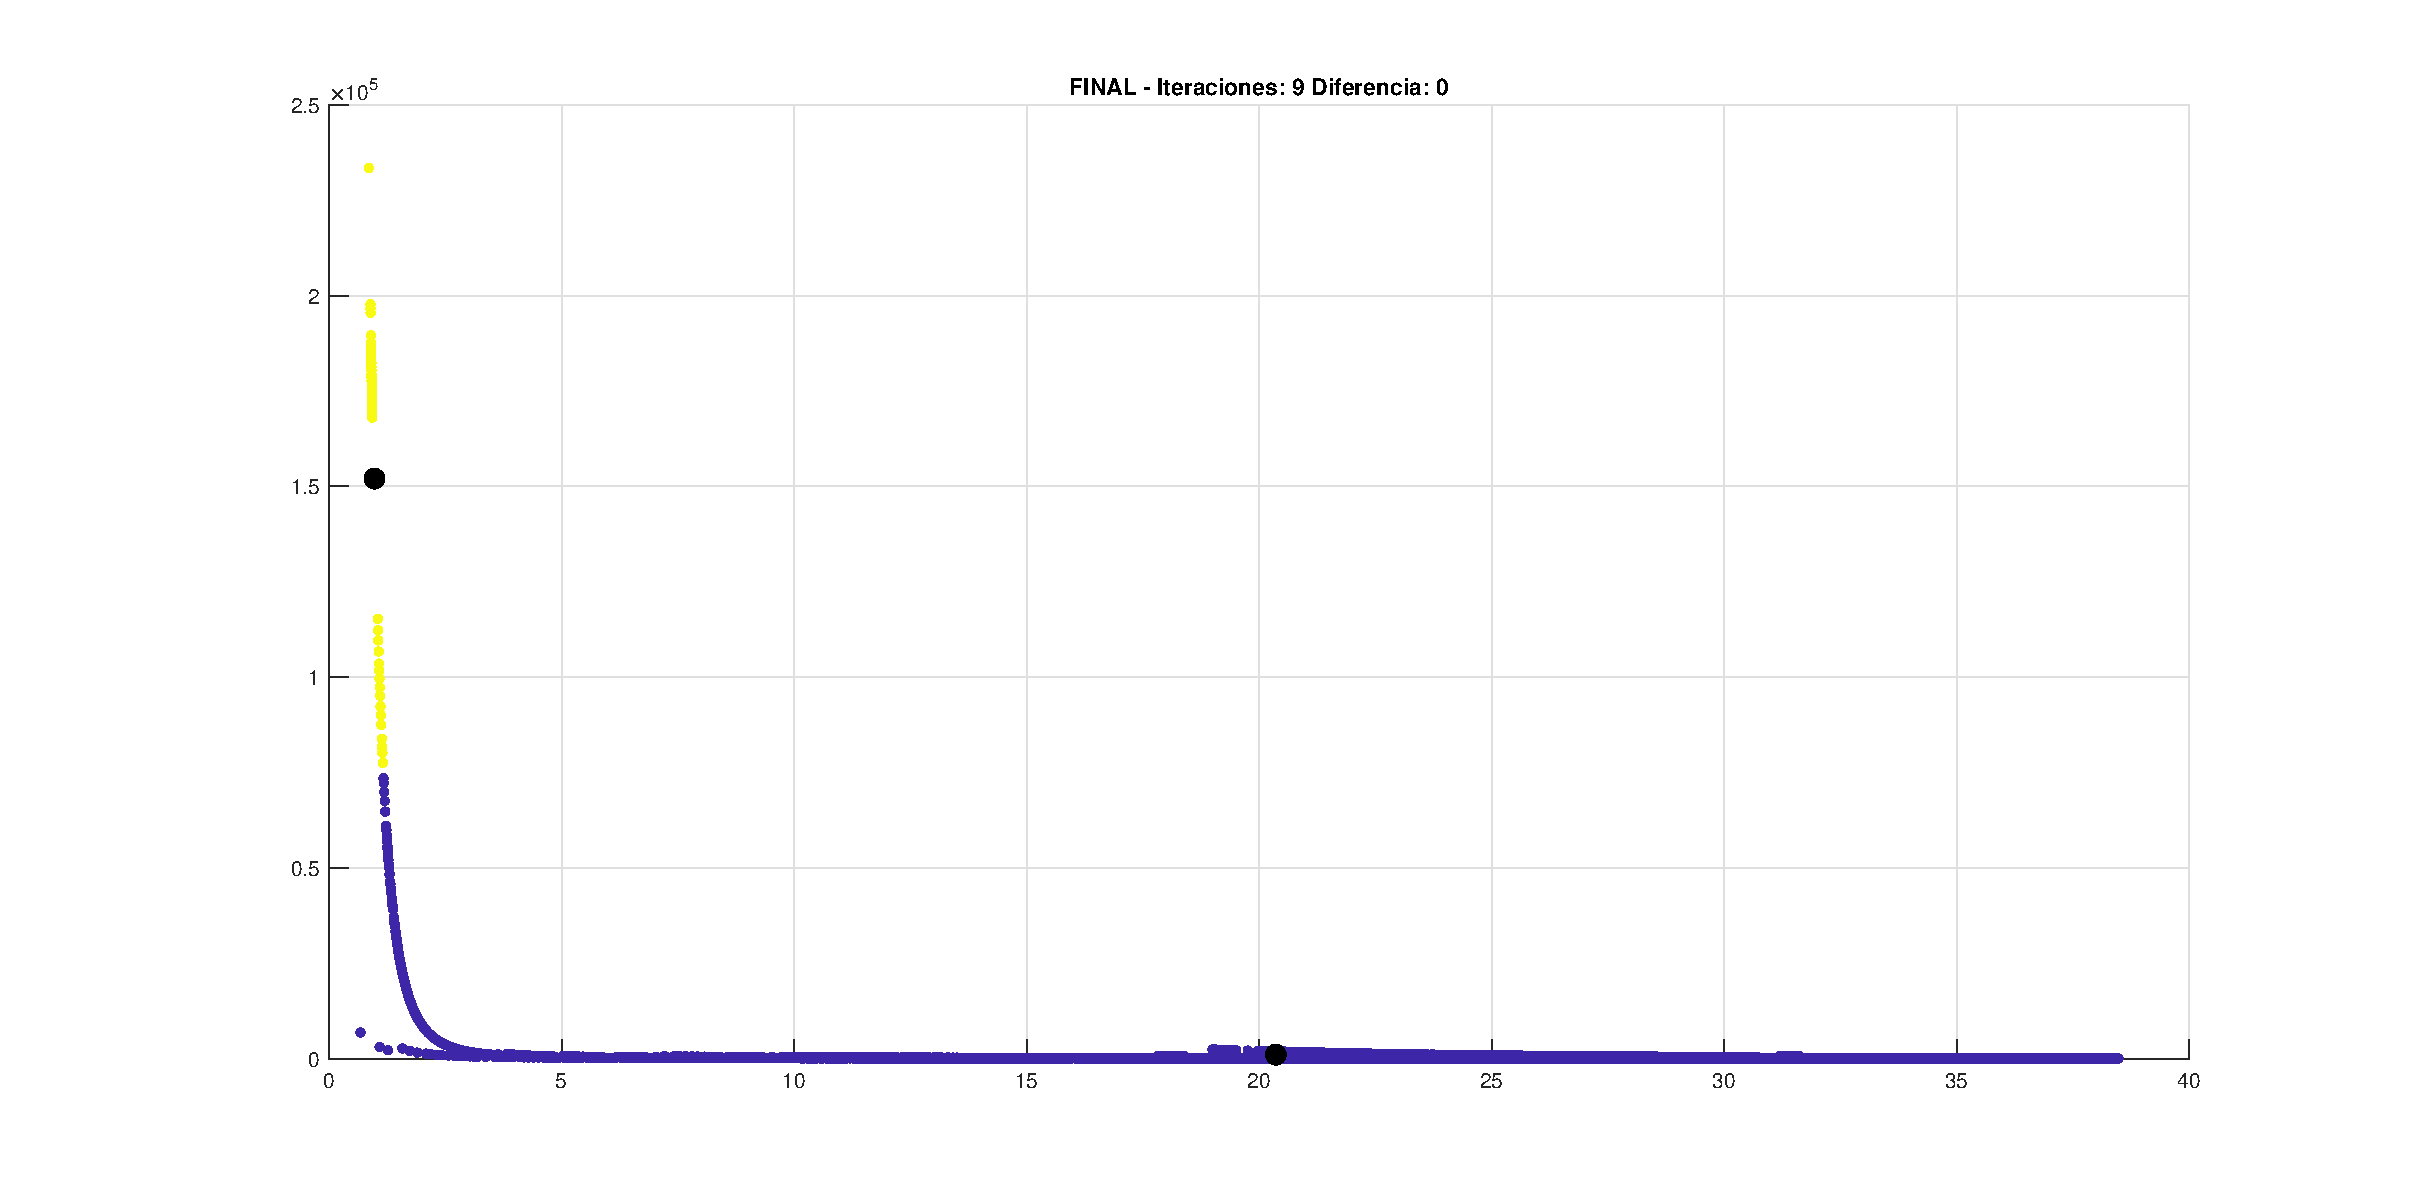
\includegraphics[width=0.90\textwidth]{figuras/k_means_time_1and2_sano_ictal.eps}
    \caption{Gráfica de agrupamiento por k-means de señales bioeléctricas de las características 1 y 2 en el dominio del tiempo  de actividad ictal y no ictal.}
    \label{fig: k_means_Time_1_2}
\end{figure}
\begin{figure}[H]
    \centering
    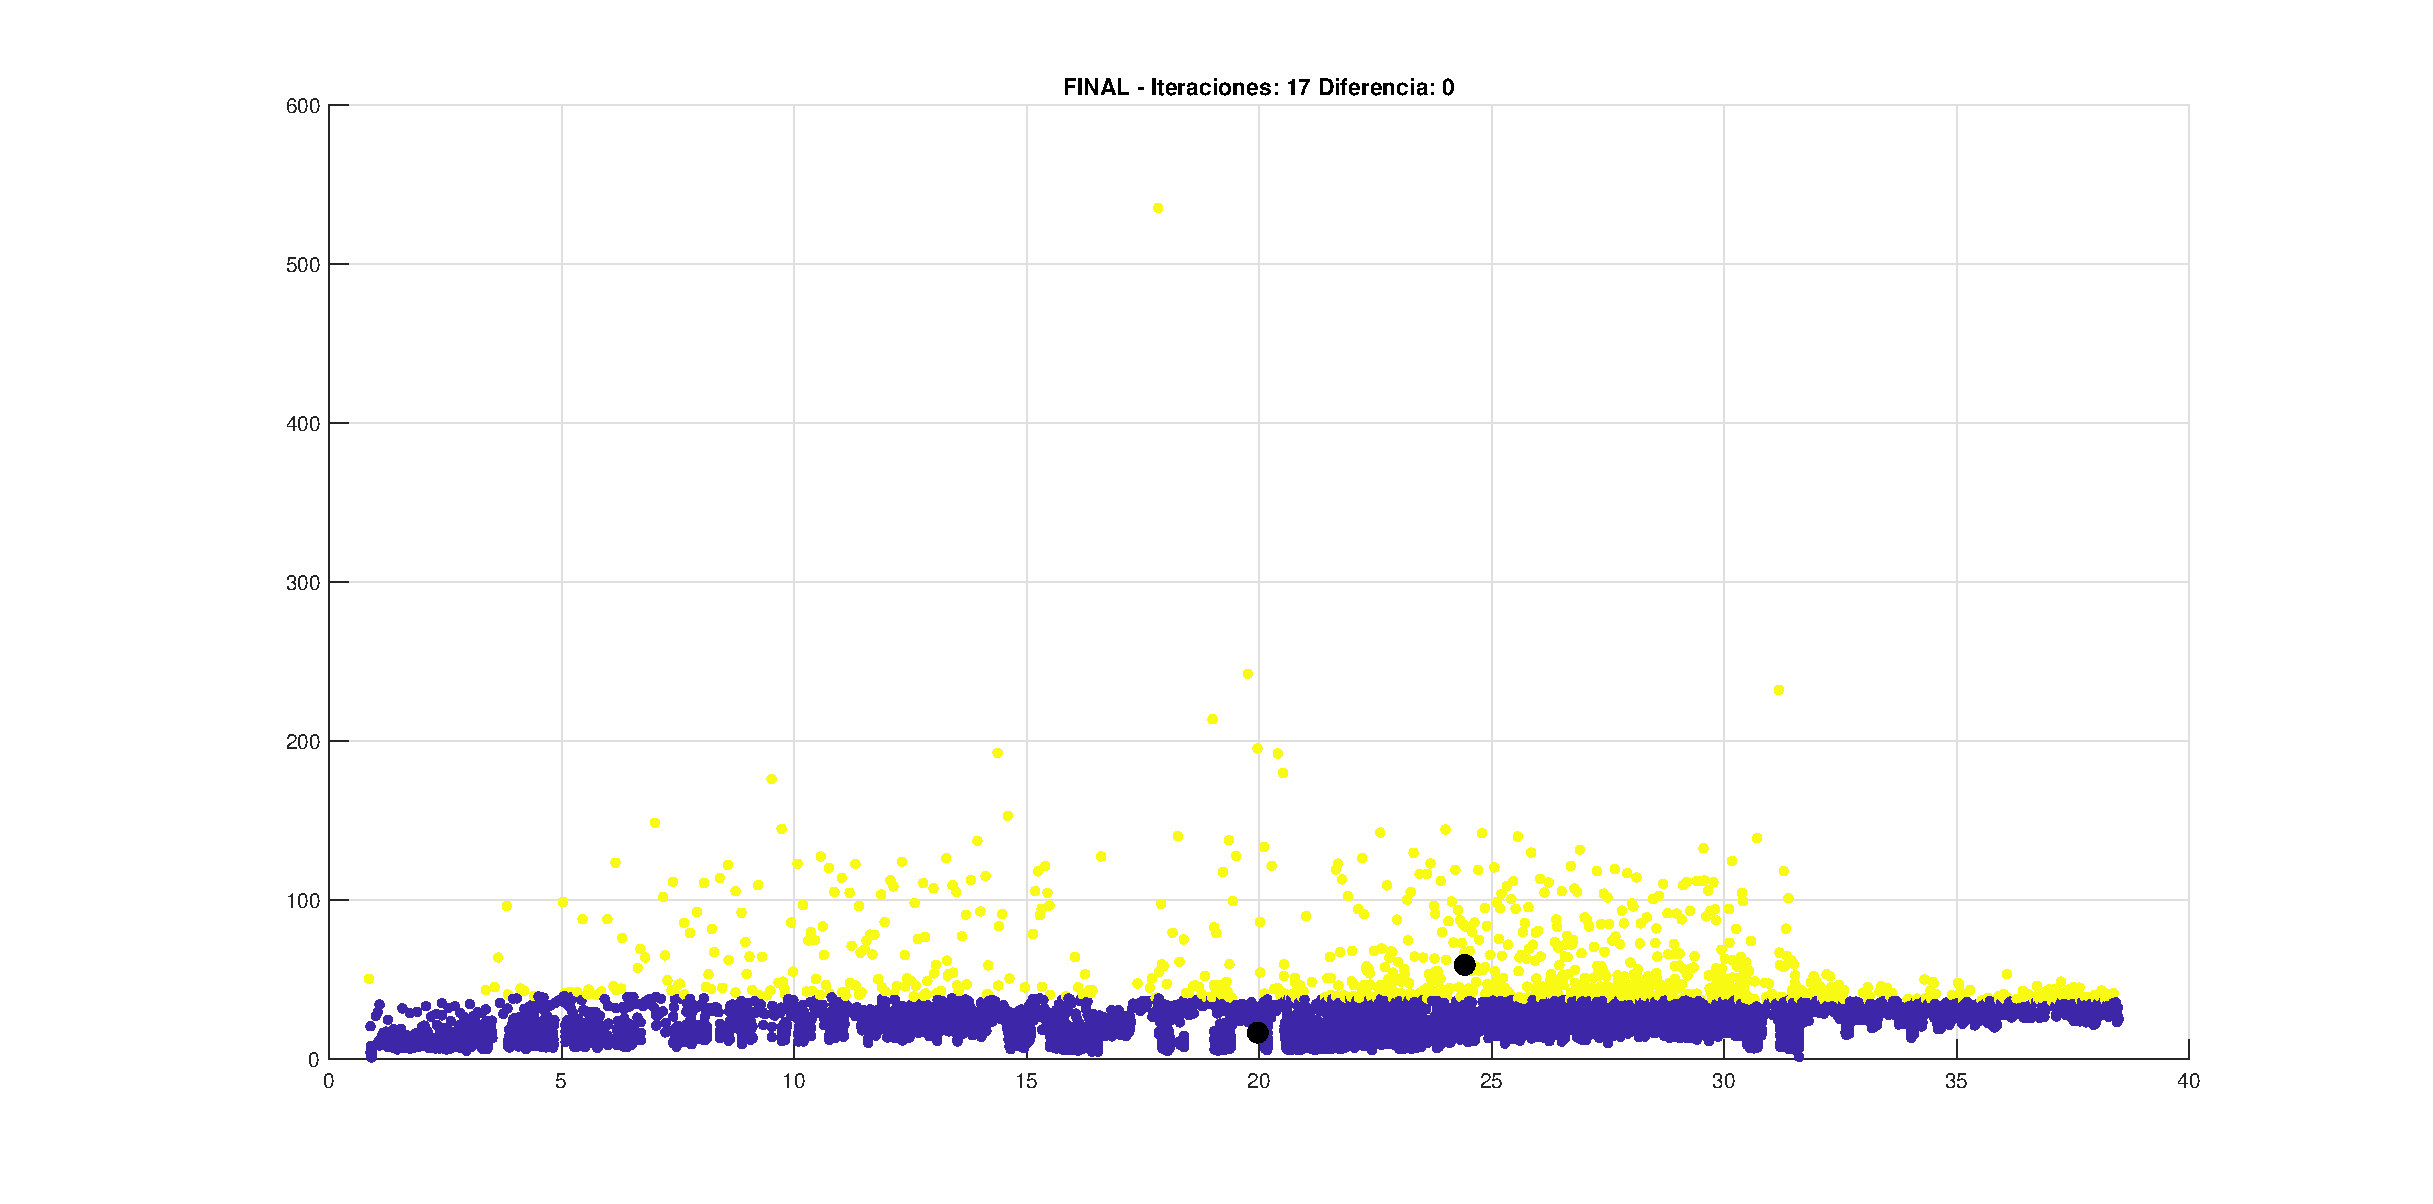
\includegraphics[width=0.90\textwidth]{figuras/k_means_time_1and4_sano_ictal.eps}
    \caption{Gráfica de agrupamiento por k-means de señales bioeléctricas de las características 1 y 4 en el dominio del tiempo de actividad ictal y no ictal.}
    \label{fig: k_means_time_1_4}
\end{figure}
\begin{figure}[H]
    \centering
    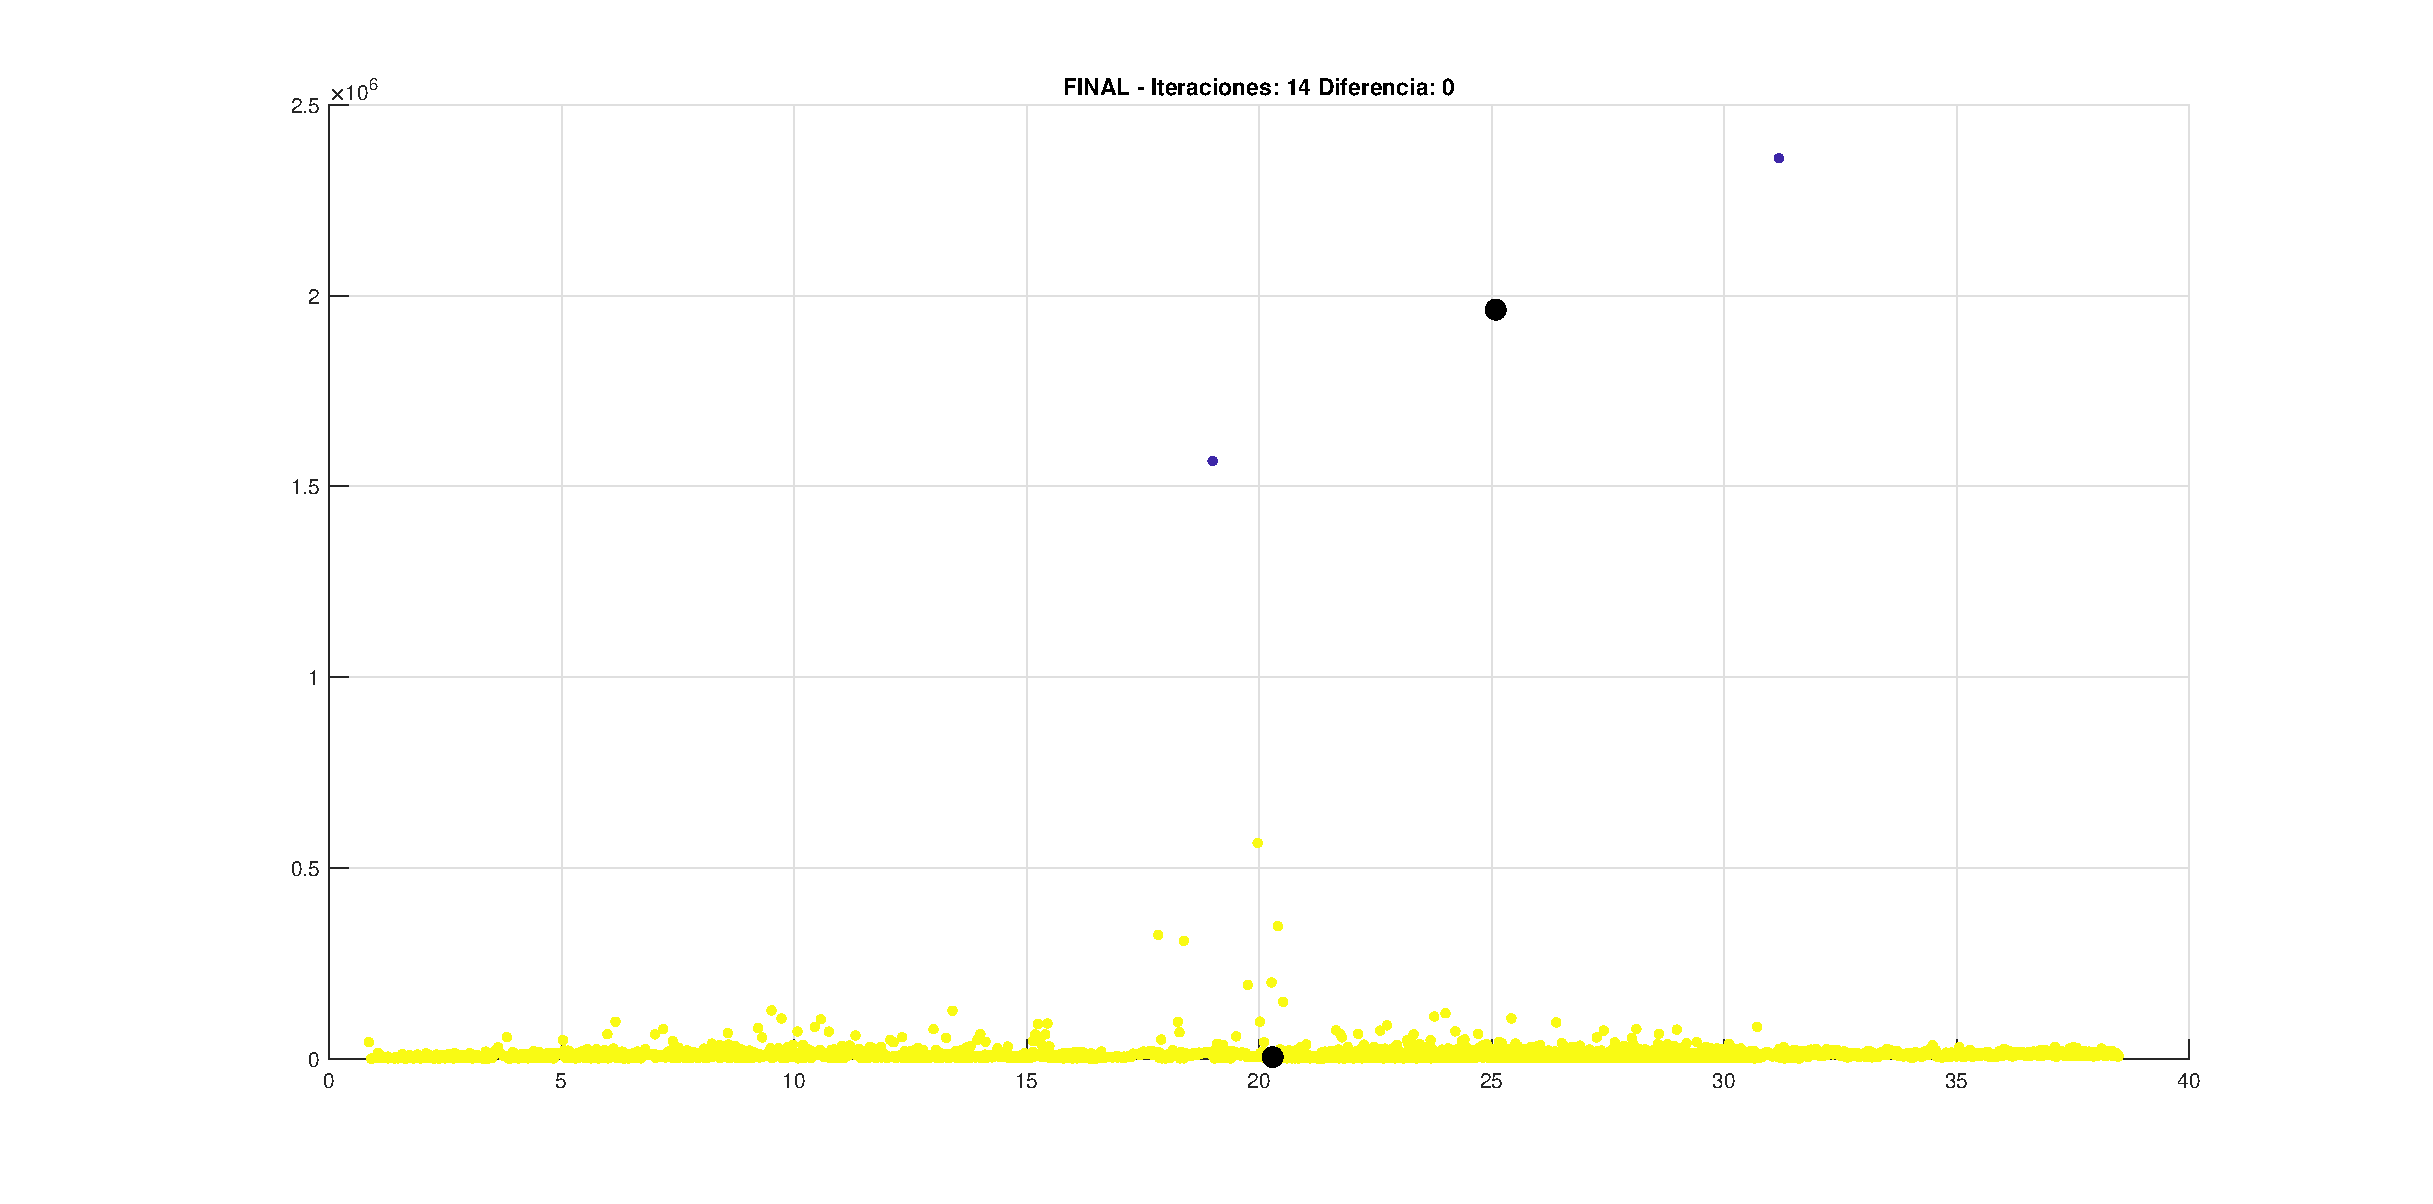
\includegraphics[width=0.90\textwidth]{figuras/k_means_time_1and5_sano_ictal.eps}
    \caption{Gráfica de agrupamiento por k-means de señales bioeléctricas de las características 1 y 5 en el dominio del tiempo de actividad ictal y no ictal.}
    \label{fig: k_means_time_1_5}
\end{figure}
\begin{figure}[H]
    \centering
    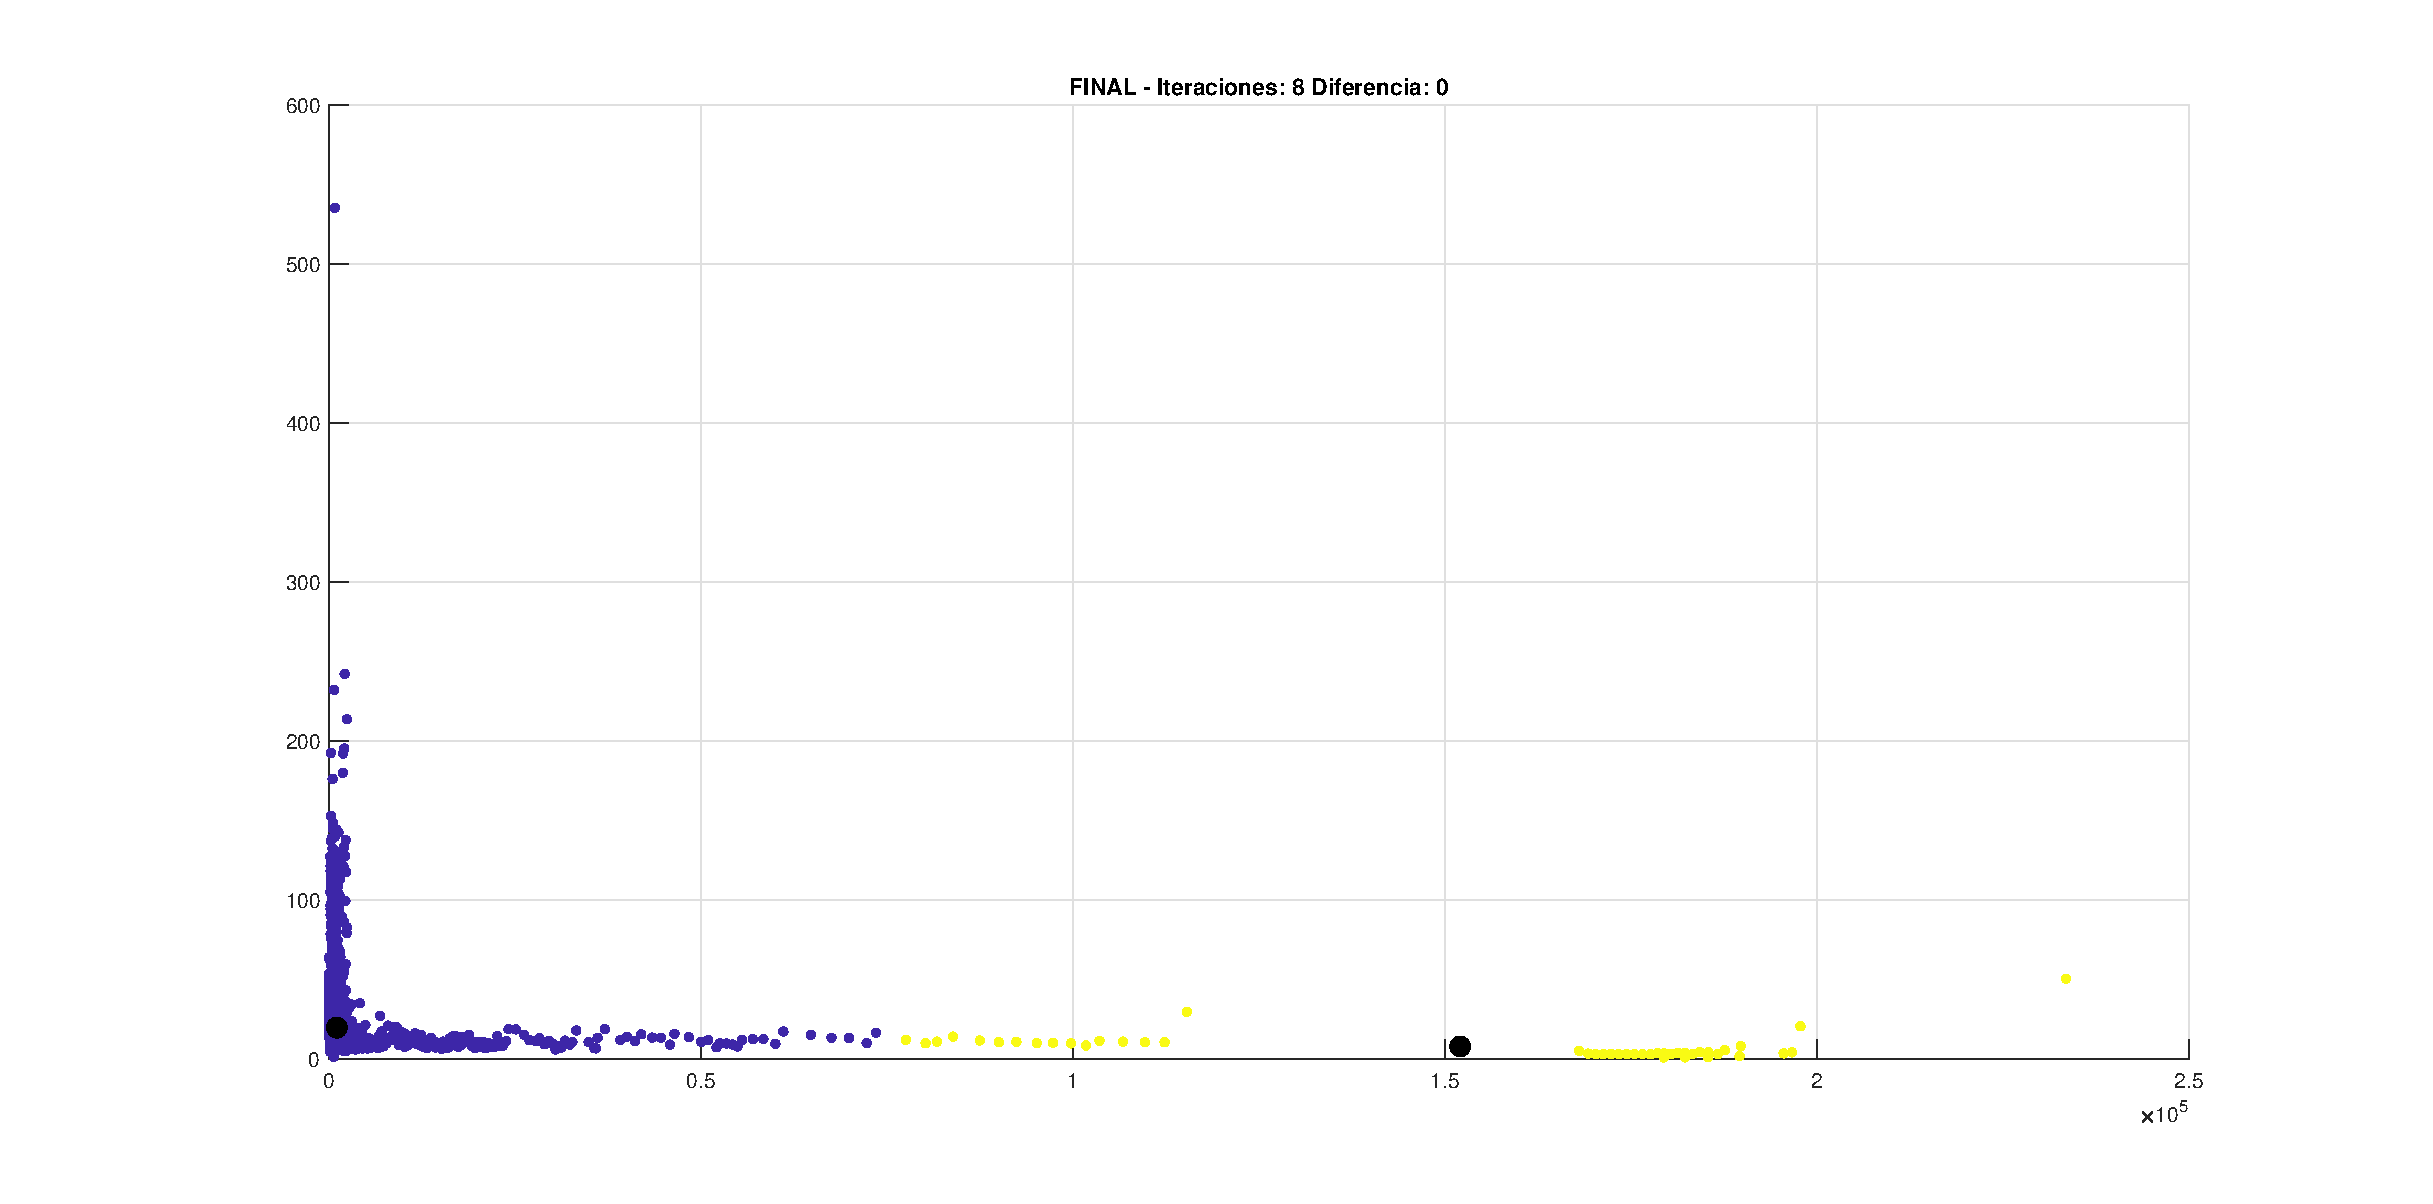
\includegraphics[width=0.90\textwidth]{figuras/k_means_time_2and4_sano_ictal.eps}
    \caption{Gráfica de agrupamiento por k-means de señales bioeléctricas de las características 2 y 4 en el dominio del tiempo de actividad ictal y no ictal.}
    \label{fig: k_means_time_2_4}
\end{figure}
\begin{figure}[H]
    \centering
    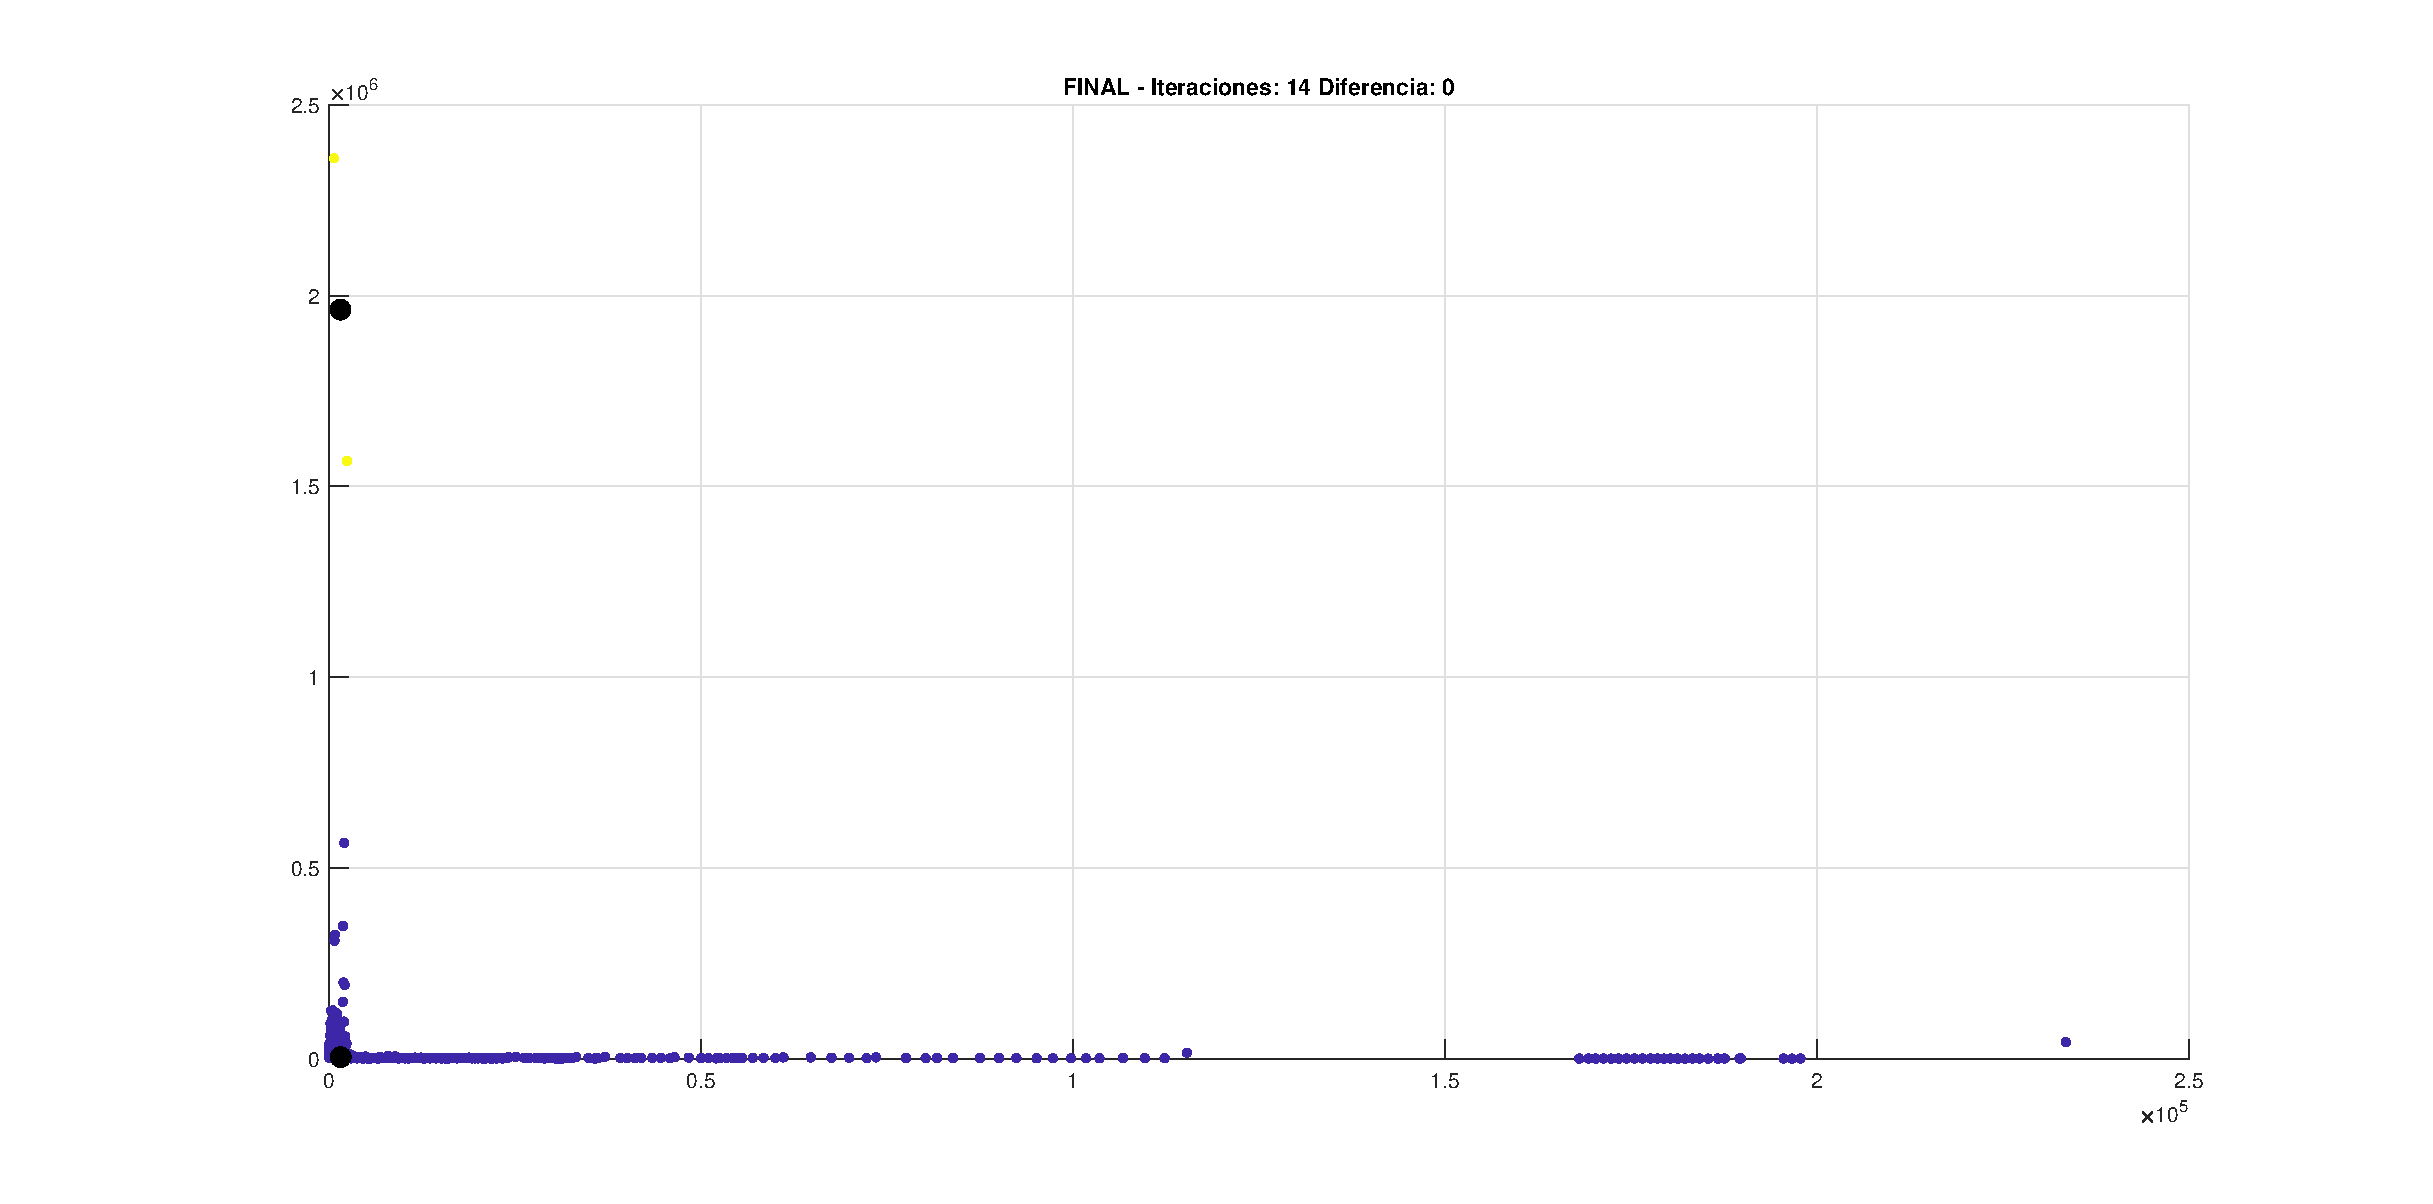
\includegraphics[width=0.90\textwidth]{figuras/k_means_time_2and5_sano_ictal.eps}
    \caption{Gráfica de agrupamiento por k-means de señales bioeléctricas de las características 2 y 5 en el dominio del tiempo de actividad ictal y no ictal.}
    \label{fig: k_means_time_2_5}
\end{figure}
\begin{figure}[H]
    \centering
    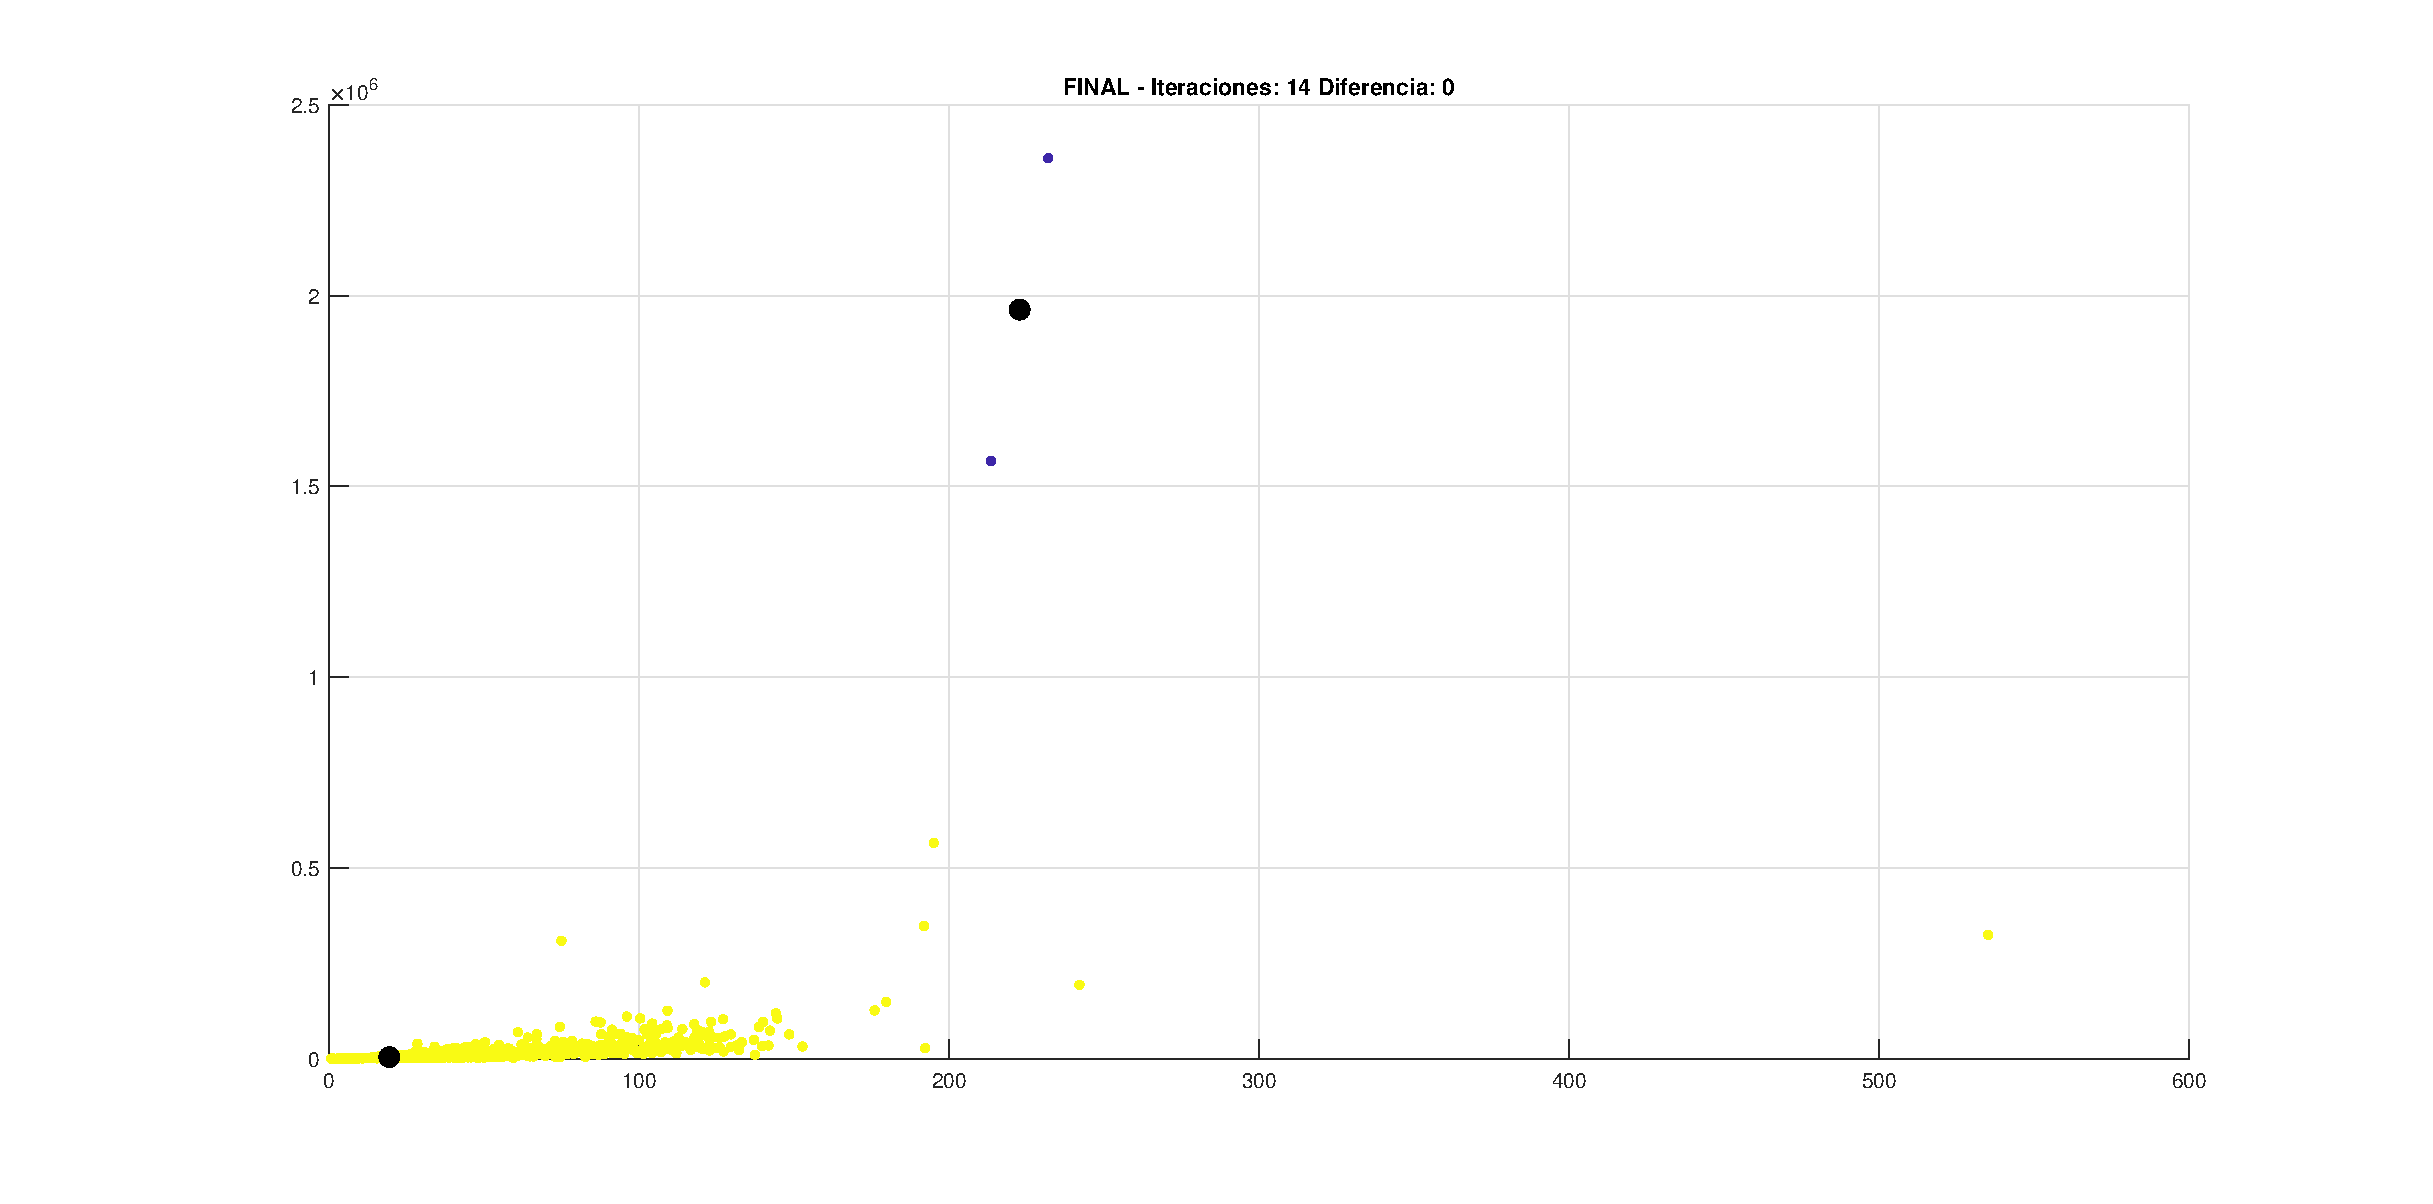
\includegraphics[width=0.90\textwidth]{figuras/k_means_time_4and5_sano_ictal.eps}
    \caption{Gráfica de agrupamiento por k-means de señales bioeléctricas de las características 4 y 5 en el dominio del tiempo de actividad ictal y no ictal.}
    \label{fig: k_means_time_4_5}
\end{figure}


\section{Análisis de Grupos en el Dominio de Frecuencia}
En el análisis de agrupamiento de señales EEG en el dominio de la frecuencia se trabajaron con las siguientes características:

\begin{enumerate}
    \item $\frac{\theta}{\alpha}$
    \item $\frac{\beta}{\alpha}$
    \item $\frac{\theta}{\beta}$
    \item $\frac{(\theta + \alpha)}{\beta}$
    \item $\frac{(\theta + \alpha)}{(\alpha + \beta)}$
    \item Desviación estándar
\end{enumerate}

%, \ref{fig: k_means_freq_1_3}, \ref{fig: k_means_freq_1_4}, \ref{fig: k_means_freq_1_5}, \ref{fig: k_means_freq_1_6}, \ref{fig: k_means_freq_2_3}, \ref{fig: k_means_freq_2_4}, \ref{fig: k_means_freq_2_5}, \ref{fig: k_means_freq_2_6}, \ref{fig: k_means_freq_3_4}, \ref{fig: k_means_freq_3_5}, \ref{fig: k_means_freq_3_6}, \ref{fig: k_means_freq_4_5},\ref{fig: k_means_freq_4_6} y

Los resultados fueron satisfactorios, como se puede observar en las Figuras~\ref{fig: k_means_freq_1_2} -  \ref{fig: k_means_freq_5_6}. Los datos forman un contorno similar a una elipse estirada por uno o dos bordes. Este patrón de agrupación resultó en una correcta separación de los datos en dos grupos, que consisten en señales EEG de individuos con actividad epiléptica y personas sanas. 

La capacidad de K-means para realizar esta separación respalda la validez de los resultados y sugiere la utilidad de las características de frecuencia en la discriminación entre individuos con actividad epiléptica y personas sanas, además de, poder notar que para este dominio la densidad de datos es muy similar para cada grupo. Por lo que el tener una mayor cantidad de datos y de manera diversificada (distintos pacientes) sin duda alguna se obtendrá una predicción excelente. 

Para las figuras anteriormente mencionadas en esta sección, cabe mencionar que con la transición entre cada grupo, se aprecia una disminución en la densidad de datos de manera gradual y significativa. Lo cual es esperado, ya que las grabaciones por parte de HUMANA contienen segmentos donde el paciente no esta pasando por un episodio epiléptico, lo que se interpretar como ruido en las características de su clase (ictal).



\begin{figure}[H]
    \centering
    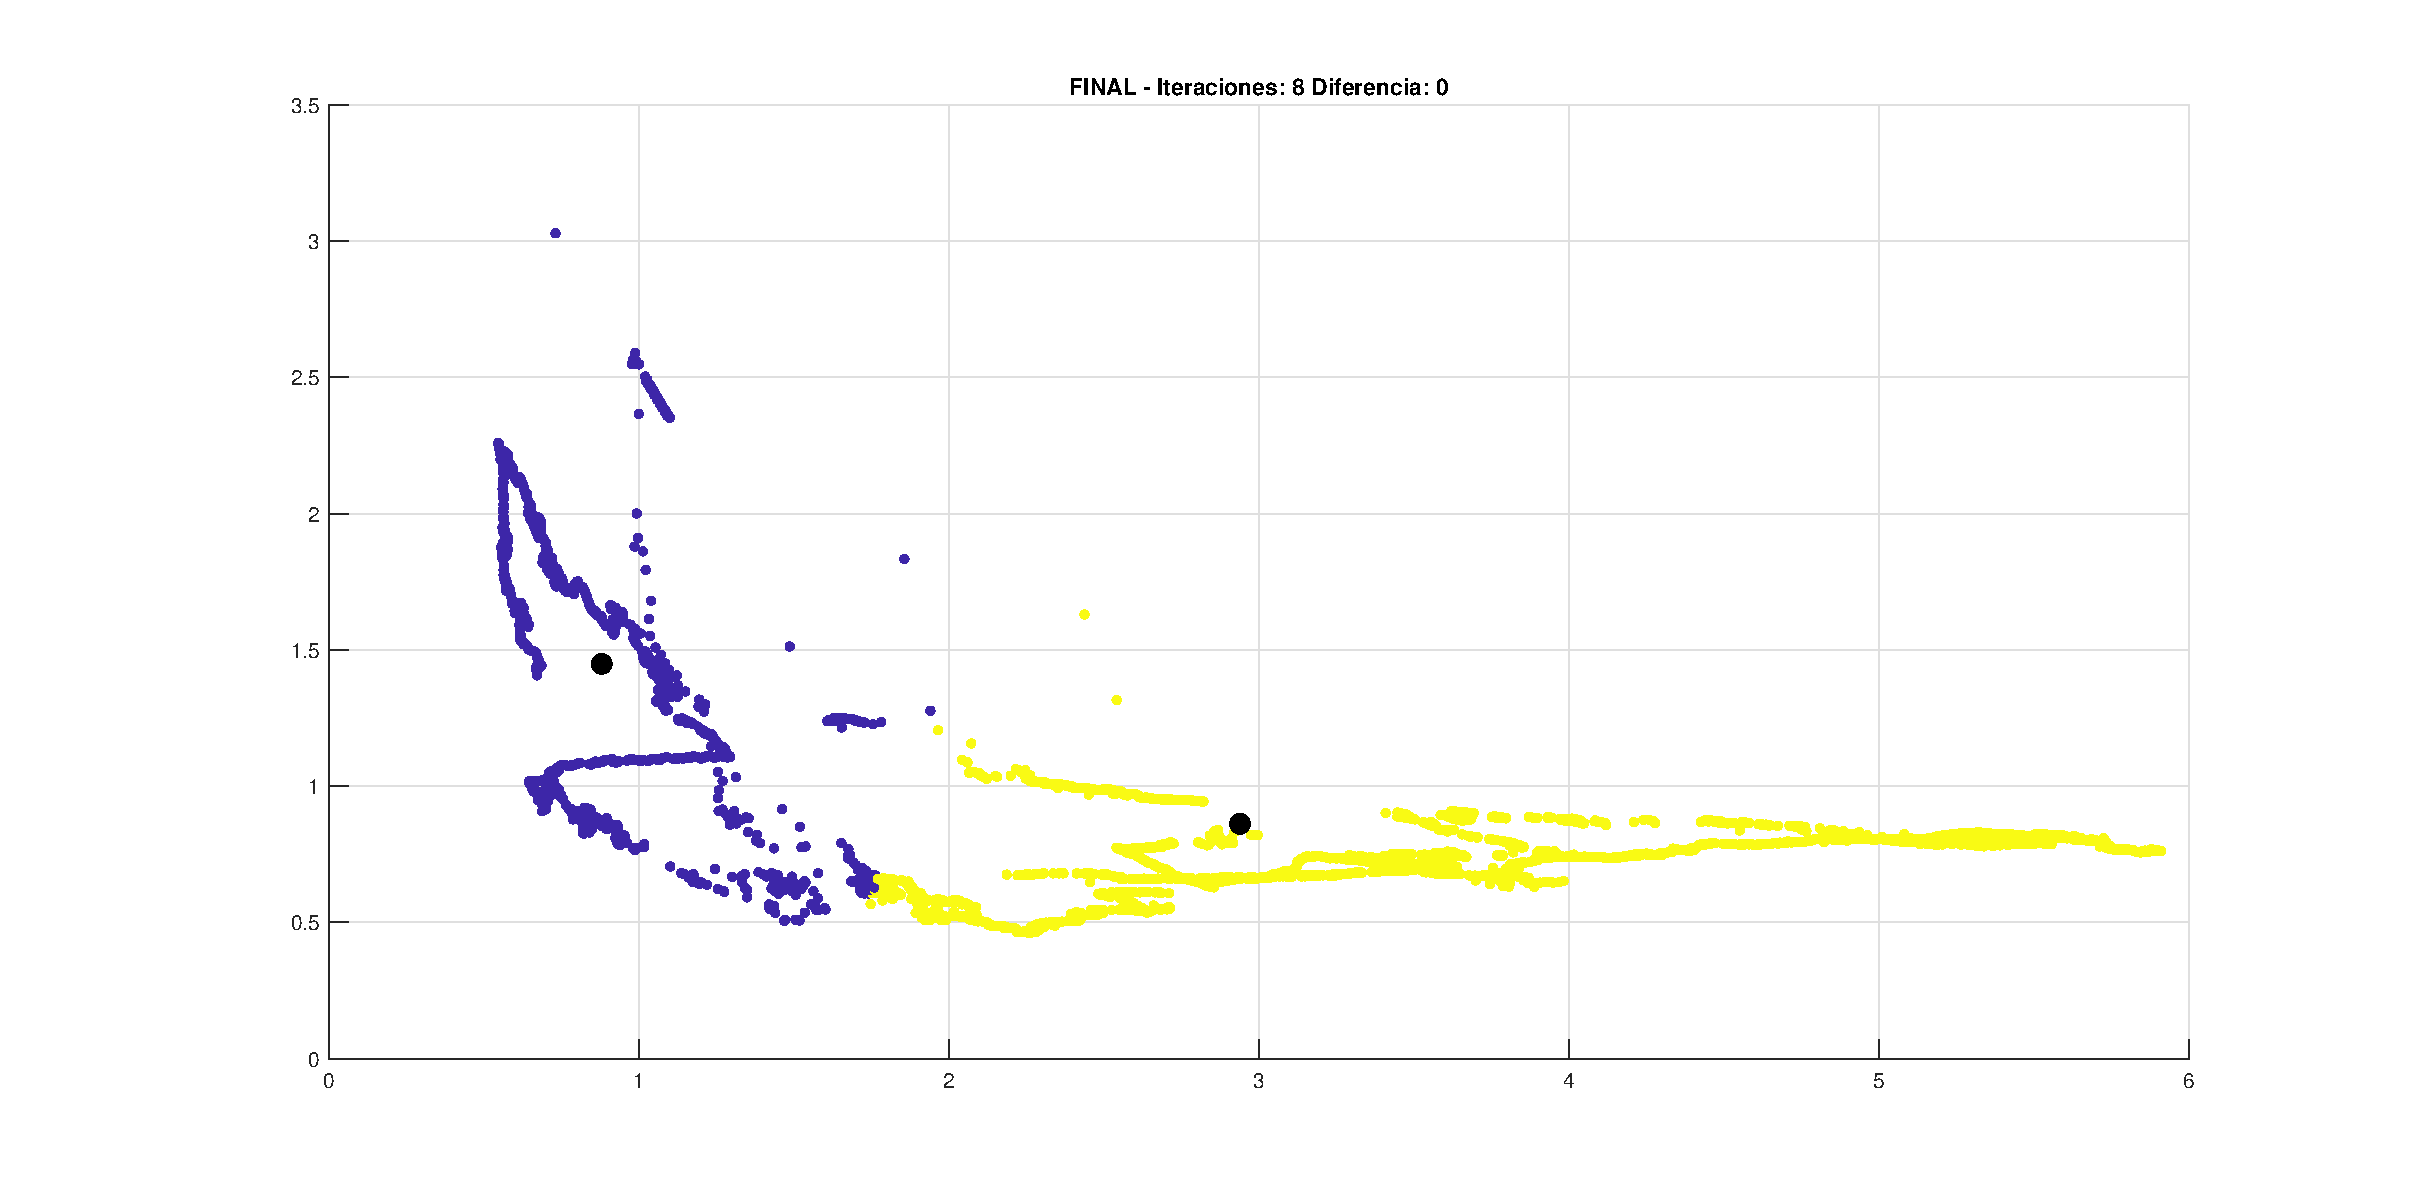
\includegraphics[width=0.90\textwidth]{figuras/k_means_freq_1and2_sano_ictal.eps}
    \caption{Gráfica de agrupamiento por k-means de señales bioeléctricas de las características 1 y 2 en el dominio de la frecuencia de actividad ictal y no ictal.}
    \label{fig: k_means_freq_1_2}
\end{figure}
\begin{figure}[H]
    \centering
    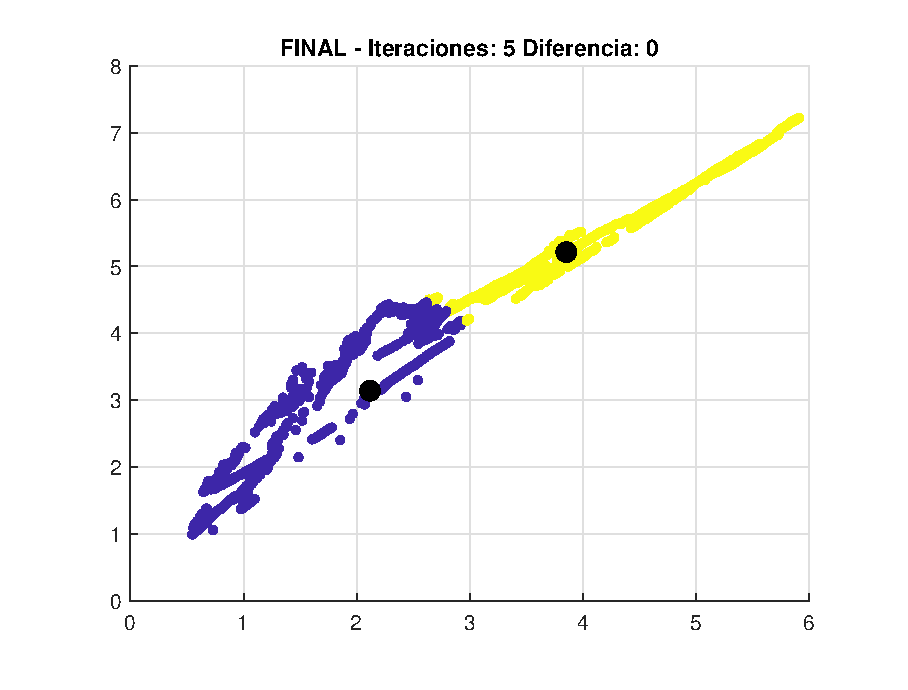
\includegraphics[width=0.90\textwidth]{figuras/k_means_freq_1and3_sano_ictal.eps}
    \caption{Gráfica de agrupamiento por k-means de señales bioeléctricas de las características 1 y 3 en el dominio de la frecuencia de actividad ictal y no ictal.}
    \label{fig: k_means_freq_1_3}
\end{figure}
\begin{figure}[H]
    \centering
    \includegraphics[width=0.90\textwidth]{figuras/k_means_freq_1and4_sano_ictal.eps}
    \caption{Gráfica de agrupamiento por k-means de señales bioeléctricas de las características 1 y 4 en el dominio de la frecuencia de actividad ictal y no ictal.}
    \label{fig: k_means_freq_1_4}
\end{figure}
\begin{figure}[H]
    \centering
    \includegraphics[width=0.8\textwidth]{figuras/k_means_freq_1and5_sano_ictal.eps}
    \caption{Gráfica de agrupamiento por k-means de señales bioeléctricas de las características 1 y 5  en el dominio de la frecuencia de actividad ictal y no ictal.}
    \label{fig: k_means_freq_1_5}
\end{figure}
\begin{figure}[H]
    \centering
    \includegraphics[width=0.8\textwidth]{figuras/k_means_freq_1and6_sano_ictal.eps}
    \caption{Gráfica de agrupamiento por k-means de señales bioeléctricas de las características 1 y 6 en el dominio de la frecuencia de actividad ictal y no ictal.}
    \label{fig: k_means_freq_1_6}
\end{figure}
\begin{figure}[H]
    \centering
    \includegraphics[width=0.8\textwidth]{figuras/k_means_freq_2and3_sano_ictal.eps}
    \caption{Gráfica de agrupamiento por k-means de señales bioeléctricas de las características 2 y 3 en el dominio de la frecuencia de actividad ictal y no ictal.}
    \label{fig: k_means_freq_2_3}
\end{figure}
\begin{figure}[H]
    \centering
    \includegraphics[width=0.8\textwidth]{figuras/k_means_freq_2and4_sano_ictal.eps}
    \caption{Gráfica de agrupamiento por k-means de señales bioeléctricas de las características 2 y 4 en el dominio de la frecuencia de actividad ictal y no ictal.}
    \label{fig: k_means_freq_2_4}
\end{figure}
\begin{figure}[H]
    \centering
    \includegraphics[width=0.8\textwidth]{figuras/k_means_freq_2and5_sano_ictal.eps}
    \caption{Gráfica de agrupamiento por k-means de señales bioeléctricas de las características 2 y 5 en el dominio de la frecuencia de actividad ictal y no ictal.}
    \label{fig: k_means_freq_2_5}
\end{figure}
\begin{figure}[H]
    \centering
    \includegraphics[width=0.8\textwidth]{figuras/k_means_freq_2and6_sano_ictal.eps}
    \caption{Gráfica de agrupamiento por k-means de señales bioeléctricas de las características 2 y 6 en el dominio de la frecuencia de actividad ictal y no ictal.}
    \label{fig: k_means_freq_2_6}
\end{figure}
\begin{figure}[H]
    \centering
    \includegraphics[width=0.8\textwidth]{figuras/k_means_freq_3and4_sano_ictal.eps}
    \caption{Gráfica de agrupamiento por k-means de señales bioeléctricas de las características 3 y 4 en el dominio de la frecuencia de actividad ictal y no ictal.}
    \label{fig: k_means_freq_3_4}
\end{figure}
\begin{figure}[H]
    \centering
    \includegraphics[width=0.8\textwidth]{figuras/k_means_freq_3and5_sano_ictal.eps}
    \caption{Gráfica de agrupamiento por k-means de señales bioeléctricas de las características 3 y 5 en el dominio de la frecuencia de actividad ictal y no ictal.}
    \label{fig: k_means_freq_3_5}
\end{figure}
\begin{figure}[H]
    \centering
    \includegraphics[width=0.8\textwidth]{figuras/k_means_freq_3and6_sano_ictal.eps}
    \caption{Gráfica de agrupamiento por k-means de señales bioeléctricas de las características 3 y 6 en el dominio de la frecuencia de actividad ictal y no ictal.}
    \label{fig: k_means_freq_3_6}
\end{figure}
\begin{figure}[H]
    \centering
    \includegraphics[width=0.8\textwidth]{figuras/k_means_freq_4and5_sano_ictal.eps}
    \caption{Gráfica de agrupamiento por k-means de señales bioeléctricas de las características 4 y 5 en el dominio de la frecuencia de actividad ictal y no ictal.}
    \label{fig: k_means_freq_4_5}
\end{figure}
\begin{figure}[H]
    \centering
    \includegraphics[width=0.8\textwidth]{figuras/k_means_freq_4and6_sano_ictal.eps}
    \caption{Gráfica de agrupamiento por k-means de señales bioeléctricas de las características 4 y 6 en el dominio de la frecuencia de actividad ictal y no ictal.}
    \label{fig: k_means_freq_4_6}
\end{figure}
\begin{figure}[H]
    \centering
    \includegraphics[width=0.8\textwidth]{figuras/k_means_freq_5and6_sano_ictal.eps}
    \caption{Gráfica de agrupamiento por k-means de señales bioeléctricas de las características 5 y 6 en el dominio de la frecuencia de actividad ictal y no ictal.}
    \label{fig: k_means_freq_5_6}
\end{figure}



\section{Análisis de Grupos en el Dominio de Wavelets}
En esta sección, se aborda el análisis de grupos resultantes de la aplicación de técnicas de procesamiento en el dominio de wavelets. Se destacan las siguientes características utilizadas en el análisis:

\begin{enumerate}
    \item Potencia
    \item Desviación
    \item Asimetría
    \item Media
    \item Curtosis
    \item Cruces por cero (ZC)
\end{enumerate}

%, \ref{fig: k_means_wave_1_3}, \ref{fig: k_means_wave_1_4}, \ref{fig: k_means_wave_1_5}, \ref{fig: k_means_wave_1_6},

%, \ref{fig: k_means_wave_4_5}, \ref{fig: k_means_wave_4_6} y
 La identificación de dos grupos de señales bioeléctricas que están ampliamente separados en el espacio de características es un hallazgo de gran relevancia, como se observa en las Figuras~\ref{fig: k_means_wave_1_2} - \ref{fig: k_means_wave_2_4}, \ref{fig: k_means_wave_2_6}, \ref{fig: k_means_wave_3_4}, \ref{fig: k_means_wave_3_6} - \ref{fig: k_means_wave_5_6}. Esta distinción evidente indica que las características analizadas, como la potencia, desviación, asimetría, media, curtosis y cruces por cero (ZC), son altamente discriminatorias entre las clases ictal y sana. Esta observación respalda la utilidad de estas características en la detección y diferenciación de estados epilépticos y salud.

La agrupación de datos en dos grupos cercanos, pero con diferentes características de densidad, también presenta un aspecto interesante, como se observar en las Figuras~\ref{fig: k_means_wave_2_3}, \ref{fig: k_means_wave_2_5} y \ref{fig: k_means_wave_3_5}. La concentración de datos en una región más pequeña en un grupo y su expansión en el otro indican que, si bien estos grupos están próximos, aún mantienen diferencias notables. Esta observación puede ser esclarecedora para la comprensión de las variaciones sutiles en las señales bioeléctricas y cómo estas variaciones pueden influir en la clasificación.

\begin{figure}[H]
    \centering
    \includegraphics[width=0.90\textwidth]{figuras/k_means_wavelet_1and2_sano_ictal.eps}
    \caption{Gráfica de agrupamiento por k-means de señales bioeléctricas de las características 1 y 2 tipo wavelets de actividad ictal y no ictal.}
    \label{fig: k_means_wave_1_2}
\end{figure}
\begin{figure}[H]
    \centering
    \includegraphics[width=0.8\textwidth]{figuras/k_means_wavelet_1and3_sano_ictal.eps}
    \caption{Gráfica de agrupamiento por k-means de señales bioeléctricas de las características 1 y 3 tipo wavelets de actividad ictal y no ictal.}
    \label{fig: k_means_wave_1_3}
\end{figure}
\begin{figure}[H]
    \centering
    \includegraphics[width=0.8\textwidth]{figuras/k_means_wavelet_1and4_sano_ictal.eps}
    \caption{Gráfica de agrupamiento por k-means de señales bioeléctricas de las características 1 y 4  tipo wavelets de actividad ictal y no ictal.}
    \label{fig: k_means_wave_1_4}
\end{figure}
\begin{figure}[H]
    \centering
    \includegraphics[width=0.8\textwidth]{figuras/k_means_wavelet_1and5_sano_ictal.eps}
    \caption{Gráfica de agrupamiento por k-means de señales bioeléctricas de las características 1 y 5 tipo wavelets de actividad ictal y no ictal.}
    \label{fig: k_means_wave_1_5}
\end{figure}
\begin{figure}[H]
    \centering
    \includegraphics[width=0.8\textwidth]{figuras/k_means_wavelet_1and6_sano_ictal.eps}
    \caption{Gráfica de agrupamiento por k-means de señales bioeléctricas de las características 1 y 6 tipo wavelets de actividad ictal y no ictal.}
    \label{fig: k_means_wave_1_6}
\end{figure}
\begin{figure}[H]
    \centering
    \includegraphics[width=0.8\textwidth]{figuras/k_means_wavelet_2and3_sano_ictal.eps}
    \caption{Gráfica de agrupamiento por k-means de señales bioeléctricas de las características 2 y 3 tipo wavelets de actividad ictal y no ictal.}
    \label{fig: k_means_wave_2_3}
\end{figure}
\begin{figure}[H]
    \centering
    \includegraphics[width=0.8\textwidth]{figuras/k_means_wavelet_2and4_sano_ictal.eps}
    \caption{Gráfica de agrupamiento por k-means de señales bioeléctricas de las características 2 y 4 tipo wavelets de actividad ictal y no ictal.}
    \label{fig: k_means_wave_2_4}
\end{figure}
\begin{figure}[H]
    \centering
    \includegraphics[width=0.8\textwidth]{figuras/k_means_wavelet_2and5_sano_ictal.eps}
    \caption{Gráfica de agrupamiento por k-means de señales bioeléctricas de las características 2 y 5 tipo wavelets de actividad ictal y no ictal.}
    \label{fig: k_means_wave_2_5}
\end{figure}
\begin{figure}[H]
    \centering
    \includegraphics[width=0.8\textwidth]{figuras/k_means_wavelet_2and6_sano_ictal.eps}
    \caption{Gráfica de agrupamiento por k-means de señales bioeléctricas de las características 2 y 6 tipo wavelets de actividad ictal y no ictal.}
    \label{fig: k_means_wave_2_6}
\end{figure}
\begin{figure}[H]
    \centering
    \includegraphics[width=0.8\textwidth]{figuras/k_means_wavelet_3and4_sano_ictal.eps}
    \caption{Gráfica de agrupamiento por k-means de señales bioeléctricas de las características 3 y 4 tipo wavelets de actividad ictal y no ictal.}
    \label{fig: k_means_wave_3_4}
\end{figure}
\begin{figure}[H]
    \centering
    \includegraphics[width=0.8\textwidth]{figuras/k_means_wavelet_3and5_sano_ictal.eps}
    \caption{Gráfica de agrupamiento por k-means de señales bioeléctricas de las características 3 y 5 tipo wavelets de actividad ictal y no ictal.}
    \label{fig: k_means_wave_3_5}
\end{figure}
\begin{figure}[H]
    \centering
    \includegraphics[width=0.8\textwidth]{figuras/k_means_wavelet_3and6_sano_ictal.eps}
    \caption{Gráfica de agrupamiento por k-means de señales bioeléctricas de las características 3 y 6 tipo wavelets de actividad ictal y no ictal.}
    \label{fig: k_means_wave_3_6}
\end{figure}
\begin{figure}[H]
    \centering
    \includegraphics[width=0.8\textwidth]{figuras/k_means_wavelet_4and5_sano_ictal.eps}
    \caption{Gráfica de agrupamiento por k-means de señales bioeléctricas de las características 4 y 5 tipo wavelets de actividad ictal y no ictal.}
    \label{fig: k_means_wave_4_5}
\end{figure}
\begin{figure}[H]
    \centering
    \includegraphics[width=0.8\textwidth]{figuras/k_means_wavelet_4and6_sano_ictal.eps}
    \caption{Gráfica de agrupamiento por k-means de señales bioeléctricas de las características 4 y 6 tipo wavelets de actividad ictal y no ictal.}
    \label{fig: k_means_wave_4_6}
\end{figure}
\begin{figure}[H]
    \centering
    \includegraphics[width=0.8\textwidth]{figuras/k_means_wavelet_5and6_sano_ictal.eps}
    \caption{Gráfica de agrupamiento por k-means de señales bioeléctricas de las características 5 y 6 tipo wavelets de actividad ictal y no ictal.}
    \label{fig: k_means_wave_5_6}
\end{figure}


\chapter{Actualización de la herramienta de software para el estudio de la epilepsia}
La actualización de la herramienta de software para el estudio de la epilepsia ha resultado en una herramienta más simple de actualizar, ya que los códigos están mejor comentados lo que ayuda definitivamente para la documentación y modificación del mismo. La herramienta ahora cuenta con más programación defensiva, lo cual es de gran ayuda a que la herramienta de software para el estudio de la epilepsia no colapse cuando se produce una advertencia o error inesperado, o por el mal uso de la misma herramienta.

Con las actualizaciones hechas, la herramienta tiene las siguientes características:
\begin{itemize}
    \item Un software más liviano: al no contar con funciones y variables innecesarias, además de, contar con métodos más sofisticados para realizar tareas en especifico y funciones nativas de MATLAB que se han descontinuado. 
    \item Facilidad para manipulación de datos: para la importación y exportación de datos, ya que en la actual versión se pueden importar datos del tipo ``edf'', ``MAT'' y de la base de datos local. La exportación de datos se da en formato ``MAT'', ``XLSX'' y ``CSV''.
\end{itemize}

La presente versión de la herramienta de software para el estudio de la epilepsia concluirá siendo implementada en el trabajo de graduación de Diego Méndez titulado ``Extensión, validación y migración de una herramienta
de software para el estudio de la epilepsia para su uso en el Centro de Epilepsia y Neurocirugía Funcional (HUMANA)''~\cite{diego_2023}. Dicha implementación permitirá obtener una herramienta de software para el estudio de la epilepsia capaz de ser ejecutada en cualquier computadora siendo amigable con el usuario, además de contar con una base de datos local.  


\section{Herramienta para la evaluación visual de la tendencia}
Se añadió la herramienta ``VAT: \textit{ A Tool for Visual Assessment of (Cluster) Tendency}'' como una herramienta valiosa para la evaluación visual de la tendencia de agrupación de datos en señales bioeléctricas como se observa en la Figura~\ref{fig: Vat_toolbox}. Esta herramienta desempeñó un papel esencial al proporcionar una representación visual clara de la estructura de agrupación de datos en múltiples dimensiones. Su uso se justifica en la necesidad de comprender la tendencia de agrupación en un conjunto de características que puede ser complejo y visualmente abrumador al aplicar técnicas de agrupamiento como K-means.

\begin{figure}[H]
	\centering
	\includegraphics[width=0.6\textwidth]{figuras/39_VAT.png}
	\caption{VAT en la herramienta de software para el estudio de la epilepsia.}
	\label{fig: Vat_toolbox}
\end{figure}

Para la aplicación de VAT se utilizaron los vectores de características completos, mencionados en el capitulo anterior. 
Como se puede observar en la Figura~\ref{fig: Vat_time} no es posible determinar una cantidad de grupos para las características en el dominio del tiempo. Lo cual implica que todos los datos independientemente de su clase (ictal o sano) están muy cerca unos de otros. Permitiendo así validar de forma visual que las características en el dominio del tiempo de las señales EEG no son las más optimas. 

En el caso de las características en el dominio de la frecuencia, revelaron ser más discriminatorias como se puede observar en la Figura~\ref{fig: Vat_freq}. Se perciben varias subgrupos los cuales pertenecen a cada tipo de característica y clase. Se puede inferir que las características en el dominio de la frecuencia presentan un mejor comportamiento para realizar predicciones correctas. En cuanto a las características wavelets, son las que mejor discriminación realizan entre clases, como se puede observar en la Figura~\ref{fig: Vat_wavelet}. Dejando bastante evidente la cantidad de clases que existen en el vector de características.

En las Figuras~\ref{fig: Vat_freq} y \ref{fig: Vat_wavelet}, se puede percibir que a la fecha no se cuenta con la misma cantidad de grabaciones de personas Ictales respecto a grabaciones de personas sanas. 

La aplicación de ``VAT'' permitió una evaluación efectiva de la tendencia de agrupación en los datos de señales bioeléctricas. Los resultados generados por esta herramienta se alinearon con las expectativas teóricas y ayudaron a identificar patrones de agrupación en el conjunto de datos y visualizar el ruido que se puede encontrar entre los tipos de clases. Esta validación refuerza la fiabilidad y utilidad de la herramienta ``VAT'' en el contexto de este estudio y respalda su contribución a la comprensión de la tendencia de agrupación en señales bioeléctricas.


\begin{figure}[H]
	\centering
	\includegraphics[width=0.6\textwidth]{figuras/vat_edf_n_Uban15_time.eps}
	\caption{Resultado tras aplicar VAT al vector de características de 5 dimensiones en el dominio tiempo.}
	\label{fig: Vat_time}
\end{figure}
\begin{figure}[H]
	\centering
	\includegraphics[width=0.6\textwidth]{figuras/vat_edf_n_Uban15_freq.eps}
	\caption{Resultado tras aplicar VAT al vector de características de 6 dimensiones en el dominio frecuencia.}
	\label{fig: Vat_freq}
\end{figure}
\begin{figure}[H]
	\centering
	\includegraphics[width=0.6\textwidth]{figuras/vat_edf_n_Uban15_wavelet.eps}
	\caption{Resultado tras aplicar VAT al vector de características de 6 dimensiones en el dominio wavelets.}
	\label{fig: Vat_wavelet}
\end{figure}

\fi

% CONCLUSIONES
% ------------------------------------------------------------------------------
\ifdefined\CAPconclusiones
	\newpage
	\chapter{Conclusiones}
	\ifdefined\parpordefecto
		\defaultparformat{k-conclusiones}
	\else
		\begin{itemize}
    \item La obtención de señales bioeléctricas permitió contar con un conjunto diverso y representativo para su posterior análisis. La recopilación de datos de pacientes con epilepsia atendidos en el Instituto HUMANA y de registros capturados con el equipo de la Universidad del Valle de Guatemala proporcionó una base sólida para la investigación y el desarrollo de la herramienta de software.
    
    \item La aplicación de algoritmos de aprendizaje automático previamente desarrollados para la extracción de características de las señales EEG y EMG fue exitosa. Estos algoritmos demostraron ser efectivos en la identificación de patrones relevantes en las señales bioeléctricas y en la generación de características que sirvieron como entrada para los procesos de detección de segmentos de interés. Aunque se percibe la necesidad de contar con una mayor cantidad de datos de distintas personas por parte de HUMANA.
    
    %\item El objetivo de mejorar el proceso de detección de segmentos de interés y la generación de anotaciones relevantes se logró con éxito. La implementación de algoritmos de aprendizaje automático permitió automatizar estas tareas de manera eficiente. La herramienta de software desarrollada demostró ser capaz de identificar eventos epilépticos en las señales EEG de acuerdo con los parámetros establecidos por el Instituto HUMANA, lo que representa un avance significativo en el campo de la detección de epilepsia.
    
    \item Los análisis estadísticos realizados arrojaron resultados positivos en términos del rendimiento de los algoritmos implementados. Se pudo evaluar de manera objetiva la eficacia de la metodología propuesta y se identificaron áreas de mejora potencial. Estos análisis proporcionaron una base sólida para la toma de decisiones y la optimización de los algoritmos utilizados.
    
    \item La actualización de la herramienta de software desarrollada en fases anteriores con las mejoras implementadas en los algoritmos de clasificación y detección de segmentos de interés representa un avance significativo en la automatización de procesos clínicos relacionados con la epilepsia. Esta actualización fortalece la capacidad de la herramienta para asistir a los especialistas médicos en el diagnóstico y seguimiento de pacientes con epilepsia, lo que contribuye a una atención más eficiente y precisa.
\end{itemize}
	\fi
\fi

% RECOMENDACIONES
% ------------------------------------------------------------------------------
\ifdefined\CAPrecomendaciones
	\newpage
	\chapter{Recomendaciones}
	\ifdefined\parpordefecto
		\defaultparformat{l-recomendaciones}
	\else
		\begin{itemize}
    \item Se recomienda continuar la recopilación de datos de señales bioeléctricas, tanto de pacientes con epilepsia como de sujetos sanos, con el fin de enriquecer la base de datos y mejorar la capacidad de detección de patrones. La inclusión de un conjunto más amplio y diverso de datos permitirá una validación más robusta de los algoritmos desarrollados, añadiendo otro tipo de señales bioeléctricas como electrocardiogramas.
    
    \item Considerando el constante avance y desarrollo de algoritmos en el campo de la Inteligencia Artificial (IA) y Aprendizaje Automático (ML), se sugiere la creación de una versión de la herramienta en Python. Dada la prevalencia y la amplia disponibilidad de bibliotecas, herramientas y algoritmos en Python para IA y ML, esta iniciativa permitirá una integración más fluida y la incorporación sencilla de nuevas técnicas y avances en el campo. Python se ha consolidado como un lenguaje de programación ampliamente aceptado en el ámbito de la ciencia de datos, lo que facilitará la colaboración y el desarrollo futuro de la herramienta en un entorno más versátil y adaptable a las innovaciones en este campo en constante evolución.

    \item Se sugiere realizar una validación clínica más amplia de la herramienta de software desarrollada en entornos médicos reales. La colaboración continua con instituciones médicas, como el Instituto HUMANA, puede proporcionar una plataforma para aplicar la metodología en la práctica médica y evaluar su utilidad en el diagnóstico y tratamiento de pacientes con epilepsia.

    \item Dado el potencial de los algoritmos de aprendizaje automático para identificar patrones en señales bioeléctricas, se recomienda explorar la aplicación de esta metodología en el estudio de otros trastornos neurológicos. Investigar la detección de patrones relacionados con otras afecciones cerebrales puede ampliar significativamente el impacto y la relevancia de la investigación.
    

    
\end{itemize}
	\fi
\fi

% BIBLIOGRAFÍA
% ------------------------------------------------------------------------------
\ifdefined\CAPbibliografia
	\newpage
    \cleardoublepage\phantomsection
	\chapter{\bibname}
    \printbibliography[heading=none]
\fi

% ANEXOS
% ------------------------------------------------------------------------------
\ifdefined\CAPanexos
	\newpage
	\chapter{Anexos}
	\ifdefined\parpordefecto
		\defaultparformat{n-anexos}
	\else
		\section{Sitios web con herramienta de software y datos recolectados}
Aquí, se presentan enlaces a los sitios web específicos donde se puede acceder a la herramienta de software mejorada desarrollada durante el proyecto, así como a los conjuntos de datos recolectados a lo largo de la investigación. Este recurso facilita a los lectores y colaboradores la exploración directa de la herramienta y la revisión de los datos utilizados en el estudio, brindando una visión integral y accesible de los resultados y contribuciones generadas.

\begin{itemize}
    \item GitHub: \url{https://github.com/pat19218/Tesis_2023}
    \item Banco de datos: \href{https://drive.google.com/drive/u/1/folders/1aTNy2e-KkGNi9qVemx3-I05KnxCGLlTQ}{Drive}
\end{itemize}

\section{Pruebas con algoritmo VAT}
En la sección dedicada a las pruebas con el algoritmo VAT, se llevó a cabo un exhaustivo análisis de las características de las señales bioeléctricas en distintos dominios: frecuencia, tiempo y wavelets. Cada prueba se diseñó para evaluar la capacidad del algoritmo VAT en la identificación de tendencias de agrupamiento bajo variadas condiciones. Con el propósito de estudiar el impacto de la cantidad de épocas empleadas en el proceso, se realizaron pruebas sucesivas, incrementando gradualmente este parámetro. Este enfoque sistemático permitió una evaluación detallada de la efectividad del algoritmo en la visualización y discernimiento de patrones de agrupamiento en las señales, brindando perspectivas valiosas sobre su rendimiento en diferentes contextos y condiciones.

\subsection{VAT características en el dominio de frecuencia}
Se exploraron detalladamente los resultados obtenidos al aplicar este algoritmo para la visualización de patrones de agrupamiento en las señales bioeléctricas. La representación gráfica generada por el VAT, donde se distinguen los grupos a través de la variación de colores, proporciona una visión integral de la estructura de los datos. Aunque se observa cierta diferenciación entre los grupos, la distinción no es tan pronunciada, lo cual plantea un escenario interesante en términos de la complejidad de los patrones presentes en las señales. Esta característica, aunque implica un mayor desafío en la identificación visual de los grupos, puede brindar \textit{insights} valiosos sobre la naturaleza sutil de las relaciones entre las señales, destacando la importancia de técnicas adicionales para una interpretación más precisa y detallada como se observan en las Figuras~\ref{vat: vat_freq_100} - \ref{vat: vat_freq_2700}.

\begin{figure}[H]
	\centering
	\includegraphics[width=0.85\textwidth]{figuras/vat_freq_100.eps}
	\caption{VAT usando 100 épocas de características tipo frecuencia.}
	\label{vat: vat_freq_100}
\end{figure}
\begin{figure}[H]
	\centering
	\includegraphics[width=0.85\textwidth]{figuras/vat_freq_500.eps}
	\caption{VAT usando 500épocas de características tipo frecuencia.}
	\label{vat: vat_freq_500}
\end{figure}
\begin{figure}[H]
	\centering
	\includegraphics[width=0.85\textwidth]{figuras/vat_freq_1000.eps}
	\caption{VAT usando 1000 épocas de características tipo frecuencia.}
	\label{vat: vat_freq_1000}
\end{figure}
\begin{figure}[H]
	\centering
	\includegraphics[width=0.85\textwidth]{figuras/vat_freq_1500.eps}
	\caption{VAT usando 1500 épocas de características tipo frecuencia.}
	\label{vat: vat_freq_1500}
\end{figure}
\begin{figure}[H]
	\centering
	\includegraphics[width=0.85\textwidth]{figuras/vat_freq_2000.eps}
	\caption{VAT usando 2000 épocas de características tipo frecuencia.}
	\label{vat: vat_freq_2000}
\end{figure}
\begin{figure}[H]
\centering
\includegraphics[width=0.85\textwidth]{figuras/vat_freq_2500.eps}
\caption{VAT usando 2500 épocas de características tipo frecuencia.}
\label{vat: vat_freq_2500}
\end{figure}
\begin{figure}[H]
	\centering
	\includegraphics[width=0.85\textwidth]{figuras/vat_freq_2600.eps}
	\caption{VAT usando 2600 épocas de características tipo frecuencia.}
	\label{vat: vat_freq_2600}
\end{figure}
\begin{figure}[H]
	\centering
	\includegraphics[width=0.85\textwidth]{figuras/vat_freq_2700.eps}
	\caption{VAT usando 2700 épocas de características tipo frecuencia.}
	\label{vat: vat_freq_2700}
\end{figure}

\subsection{VAT características en el dominio de tiempo continuo}
En la exploración de las características en el dominio del tiempo continuo mediante la aplicación del algoritmo VAT, se observa una distribución particular de los datos. La representación visual destaca por la ausencia de una clara diferenciación de grupos, ya que la variación de colores revela una proximidad significativa entre todos los puntos de datos. Esta cercanía en la representación visual sugiere que las características analizadas en este contexto particular pueden no ser tan discriminatorias como se esperaba para identificar patrones distintivos de agrupamiento.Este hallazgo insta a una reflexión más profunda sobre la naturaleza de las características consideradas y la exploración de enfoques alternativos para la identificación de patrones en el dominio del tiempo continuo, como se observa en las Figuras~\ref{vat: vat_time_100} - \ref{vat: vat_time_2300}. 

\begin{figure}[H]
	\centering
	\includegraphics[width=0.85\textwidth]{figuras/vat_time_100.eps}
	\caption{VAT usando 100 épocas de características tipo tiempo continuo.}
	\label{vat: vat_time_100}
\end{figure}
\begin{figure}[H]
	\centering
	\includegraphics[width=0.85\textwidth]{figuras/vat_time_500.eps}
	\caption{VAT usando 500 épocas de características tipo tiempo continuo.}
	\label{vat: vat_time_500}
\end{figure}
\begin{figure}[H]
	\centering
	\includegraphics[width=0.85\textwidth]{figuras/vat_time_1000.eps}
	\caption{VAT usando 1000 épocas de características tipo tiempo continuo.}
	\label{vat: vat_time_1000}
\end{figure}
\begin{figure}[H]
	\centering
	\includegraphics[width=0.85\textwidth]{figuras/vat_time_1500.eps}
	\caption{VAT usando 1500 épocas de características tipo tiempo continuo.}
	\label{vat: vat_time_1500}
\end{figure}
\begin{figure}[H]
	\centering
	\includegraphics[width=0.85\textwidth]{figuras/vat_time_2000.eps}
	\caption{VAT usando 2000 épocas de características tipo tiempo continuo.}
	\label{vat: vat_time_2000}
\end{figure}
\begin{figure}[H]
	\centering
	\includegraphics[width=0.85\textwidth]{figuras/vat_time_2100.eps}
	\caption{VAT usando 2100 épocas de características tipo tiempo continuo.}
	\label{vat: vat_time_2100}
\end{figure}
\begin{figure}[H]
	\centering
	\includegraphics[width=0.85\textwidth]{figuras/vat_time_2200.eps}
	\caption{VAT usando 2200 épocas de características tipo tiempo continuo.}
	\label{vat: vat_time_2200}
\end{figure}
\begin{figure}[H]
	\centering
	\includegraphics[width=0.85\textwidth]{figuras/vat_time_2300.eps}
	\caption{VAT usando 2300 épocas de características tipo tiempo continuo.}
	\label{vat: vat_time_2300}
\end{figure}


\subsection{VAT características en el dominio de wavelets}
La aplicación del algoritmo VAT a las características extraídas en el dominio de wavelets revela resultados notables en la diferenciación de patrones en las señales bioeléctricas. La representación visual muestra una clara distinción entre dos grupos, evidenciada por la marcada variación de colores. Esta observación sugiere que las características en el dominio de wavelets utilizadas en el análisis poseen una capacidad discriminatoria sobresaliente, permitiendo una separación efectiva entre las señales asociadas a estados sanos y ictales. La nitidez en la identificación de estos grupos mediante VAT en el dominio de wavelets subraya la importancia y relevancia de estas características para el análisis y clasificación de señales bioeléctricas. Estos resultados prometedores proporcionan una base sólida para considerar el dominio de wavelets como un enfoque valioso en la identificación de patrones distintivos en señales bioeléctricas relacionadas con la epilepsia. Para ello observar las Figuras~\ref{vat: vat_wavelets_100} - \ref{vat: vat_wavelets_2300}.

\begin{figure}[H]
	\centering
	\includegraphics[width=0.85\textwidth]{figuras/vat_wavelets_100.eps}
	\caption{VAT usando 100 épocas de características tipo wavelets.}
	\label{vat: vat_wavelets_100}
\end{figure}
\begin{figure}[H]
	\centering
	\includegraphics[width=0.85\textwidth]{figuras/vat_wavelets_500.eps}
	\caption{VAT usando 500 épocas de características tipo wavelets.}
	\label{vat: vat_wavelets_500}
\end{figure}
\begin{figure}[H]
	\centering
	\includegraphics[width=0.85\textwidth]{figuras/vat_wavelets_1000.eps}
	\caption{VAT usando 1000 épocas de características tipo wavelets.}
	\label{vat: vat_wavelets_1000}
\end{figure}
\begin{figure}[H]
	\centering
	\includegraphics[width=0.85\textwidth]{figuras/vat_wavelets_1500.eps}
	\caption{VAT usando 1500 épocas de características tipo wavelets.}
	\label{vat: vat_wavelets_1500}
\end{figure}
\begin{figure}[H]
	\centering
	\includegraphics[width=0.85\textwidth]{figuras/vat_wavelets_2000.eps}
	\caption{VAT usando 2000 épocas de características tipo wavelets.}
	\label{vat: vat_wavelets_2000}
\end{figure}
\begin{figure}[H]
	\centering
	\includegraphics[width=0.85\textwidth]{figuras/vat_wavelets_2100.eps}
	\caption{VAT usando 2100 épocas de características tipo wavelets.}
	\label{vat: vat_wavelets_2100}
\end{figure}
\begin{figure}[H]
	\centering
	\includegraphics[width=0.85\textwidth]{figuras/vat_wavelets_2200.eps}
	\caption{VAT usando 2200 épocas de características tipo wavelets.}
	\label{vat: vat_wavelets_2200}
\end{figure}
\begin{figure}[H]
	\centering
	\includegraphics[width=0.85\textwidth]{figuras/vat_wavelets_2300.eps}
	\caption{VAT usando 2300 épocas de características tipo wavelets.}
	\label{vat: vat_wavelets_2300}
\end{figure}


	\fi
\fi

% GLOSARIO
% ------------------------------------------------------------------------------
\ifdefined\CAPglosario
	\newpage
	\printglossary
\fi

\end{document}